% Created by tikzDevice version 0.12.3 on 2020-04-04 16:09:59
% !TEX encoding = UTF-8 Unicode
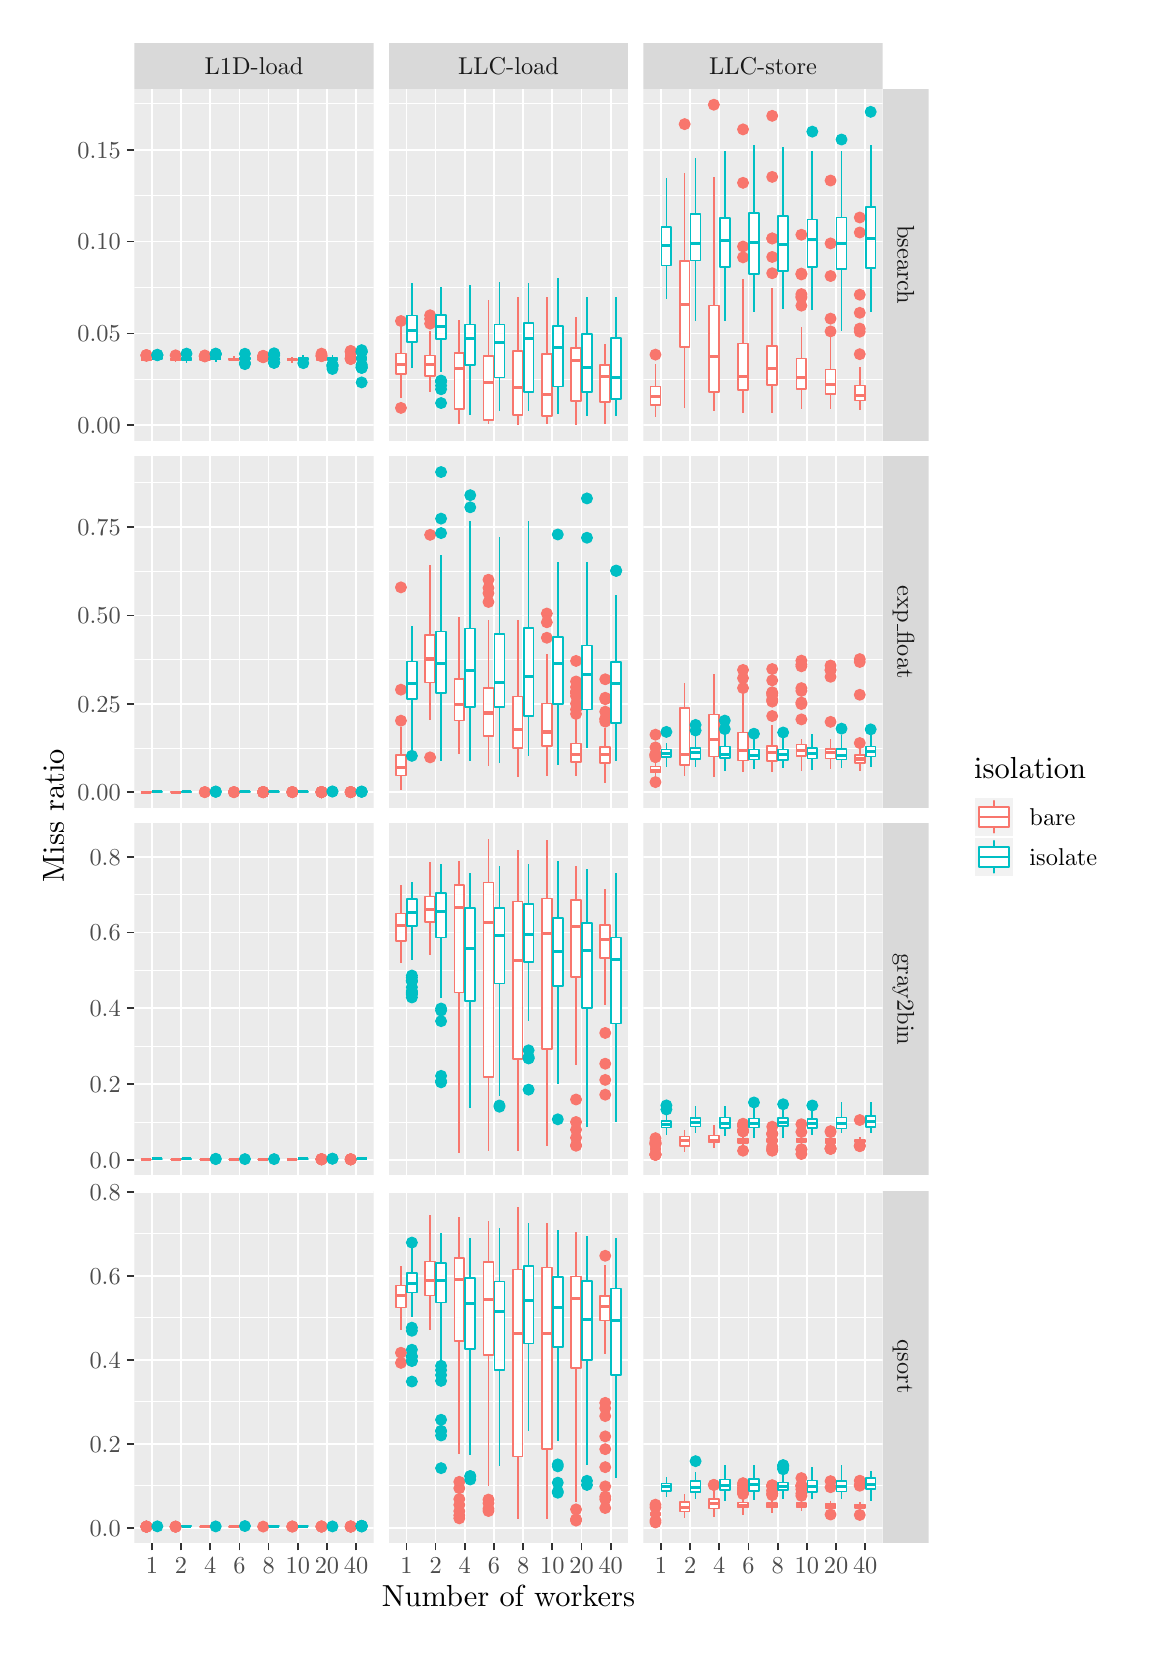
\begin{tikzpicture}[x=1pt,y=1pt]
\definecolor{fillColor}{RGB}{255,255,255}
\path[use as bounding box,fill=fillColor,fill opacity=0.00] (0,0) rectangle (397.48,578.16);
\begin{scope}
\path[clip] (  0.00,  0.00) rectangle (397.48,578.16);
\definecolor{drawColor}{RGB}{255,255,255}
\definecolor{fillColor}{RGB}{255,255,255}

\path[draw=drawColor,line width= 0.6pt,line join=round,line cap=round,fill=fillColor] (  0.00,  0.00) rectangle (397.48,578.16);
\end{scope}
\begin{scope}
\path[clip] ( 38.56,428.86) rectangle (125.03,556.09);
\definecolor{fillColor}{gray}{0.92}

\path[fill=fillColor] ( 38.56,428.86) rectangle (125.03,556.09);
\definecolor{drawColor}{RGB}{255,255,255}

\path[draw=drawColor,line width= 0.3pt,line join=round] ( 38.56,451.10) --
	(125.03,451.10);

\path[draw=drawColor,line width= 0.3pt,line join=round] ( 38.56,484.28) --
	(125.03,484.28);

\path[draw=drawColor,line width= 0.3pt,line join=round] ( 38.56,517.46) --
	(125.03,517.46);

\path[draw=drawColor,line width= 0.3pt,line join=round] ( 38.56,550.64) --
	(125.03,550.64);

\path[draw=drawColor,line width= 0.6pt,line join=round] ( 38.56,434.51) --
	(125.03,434.51);

\path[draw=drawColor,line width= 0.6pt,line join=round] ( 38.56,467.69) --
	(125.03,467.69);

\path[draw=drawColor,line width= 0.6pt,line join=round] ( 38.56,500.87) --
	(125.03,500.87);

\path[draw=drawColor,line width= 0.6pt,line join=round] ( 38.56,534.05) --
	(125.03,534.05);

\path[draw=drawColor,line width= 0.6pt,line join=round] ( 44.88,428.86) --
	( 44.88,556.09);

\path[draw=drawColor,line width= 0.6pt,line join=round] ( 55.43,428.86) --
	( 55.43,556.09);

\path[draw=drawColor,line width= 0.6pt,line join=round] ( 65.97,428.86) --
	( 65.97,556.09);

\path[draw=drawColor,line width= 0.6pt,line join=round] ( 76.52,428.86) --
	( 76.52,556.09);

\path[draw=drawColor,line width= 0.6pt,line join=round] ( 87.06,428.86) --
	( 87.06,556.09);

\path[draw=drawColor,line width= 0.6pt,line join=round] ( 97.61,428.86) --
	( 97.61,556.09);

\path[draw=drawColor,line width= 0.6pt,line join=round] (108.15,428.86) --
	(108.15,556.09);

\path[draw=drawColor,line width= 0.6pt,line join=round] (118.70,428.86) --
	(118.70,556.09);
\definecolor{drawColor}{RGB}{248,118,109}
\definecolor{fillColor}{RGB}{248,118,109}

\path[draw=drawColor,line width= 0.4pt,line join=round,line cap=round,fill=fillColor] ( 42.91,459.85) circle (  1.96);

\path[draw=drawColor,line width= 0.4pt,line join=round,line cap=round,fill=fillColor] ( 42.91,459.85) circle (  1.96);

\path[draw=drawColor,line width= 0.4pt,line join=round,line cap=round,fill=fillColor] ( 42.91,459.55) circle (  1.96);

\path[draw=drawColor,line width= 0.6pt,line join=round] ( 42.91,458.51) -- ( 42.91,459.43);

\path[draw=drawColor,line width= 0.6pt,line join=round] ( 42.91,457.90) -- ( 42.91,457.44);
\definecolor{fillColor}{RGB}{255,255,255}

\path[draw=drawColor,line width= 0.6pt,line join=round,line cap=round,fill=fillColor] ( 41.13,458.51) --
	( 41.13,457.90) --
	( 44.68,457.90) --
	( 44.68,458.51) --
	( 41.13,458.51) --
	cycle;

\path[draw=drawColor,line width= 1.1pt,line join=round] ( 41.13,458.23) -- ( 44.68,458.23);
\definecolor{drawColor}{RGB}{0,191,196}
\definecolor{fillColor}{RGB}{0,191,196}

\path[draw=drawColor,line width= 0.4pt,line join=round,line cap=round,fill=fillColor] ( 46.86,459.78) circle (  1.96);

\path[draw=drawColor,line width= 0.4pt,line join=round,line cap=round,fill=fillColor] ( 46.86,459.99) circle (  1.96);

\path[draw=drawColor,line width= 0.4pt,line join=round,line cap=round,fill=fillColor] ( 46.86,459.81) circle (  1.96);

\path[draw=drawColor,line width= 0.6pt,line join=round] ( 46.86,458.92) -- ( 46.86,459.71);

\path[draw=drawColor,line width= 0.6pt,line join=round] ( 46.86,458.36) -- ( 46.86,457.74);
\definecolor{fillColor}{RGB}{255,255,255}

\path[draw=drawColor,line width= 0.6pt,line join=round,line cap=round,fill=fillColor] ( 45.08,458.92) --
	( 45.08,458.36) --
	( 48.64,458.36) --
	( 48.64,458.92) --
	( 45.08,458.92) --
	cycle;

\path[draw=drawColor,line width= 1.1pt,line join=round] ( 45.08,458.60) -- ( 48.64,458.60);
\definecolor{drawColor}{RGB}{248,118,109}
\definecolor{fillColor}{RGB}{248,118,109}

\path[draw=drawColor,line width= 0.4pt,line join=round,line cap=round,fill=fillColor] ( 53.45,459.76) circle (  1.96);

\path[draw=drawColor,line width= 0.6pt,line join=round] ( 53.45,458.64) -- ( 53.45,459.50);

\path[draw=drawColor,line width= 0.6pt,line join=round] ( 53.45,458.00) -- ( 53.45,457.43);
\definecolor{fillColor}{RGB}{255,255,255}

\path[draw=drawColor,line width= 0.6pt,line join=round,line cap=round,fill=fillColor] ( 51.67,458.64) --
	( 51.67,458.00) --
	( 55.23,458.00) --
	( 55.23,458.64) --
	( 51.67,458.64) --
	cycle;

\path[draw=drawColor,line width= 1.1pt,line join=round] ( 51.67,458.28) -- ( 55.23,458.28);
\definecolor{drawColor}{RGB}{0,191,196}
\definecolor{fillColor}{RGB}{0,191,196}

\path[draw=drawColor,line width= 0.4pt,line join=round,line cap=round,fill=fillColor] ( 57.40,460.38) circle (  1.96);

\path[draw=drawColor,line width= 0.6pt,line join=round] ( 57.40,458.83) -- ( 57.40,459.43);

\path[draw=drawColor,line width= 0.6pt,line join=round] ( 57.40,458.09) -- ( 57.40,457.07);
\definecolor{fillColor}{RGB}{255,255,255}

\path[draw=drawColor,line width= 0.6pt,line join=round,line cap=round,fill=fillColor] ( 55.63,458.83) --
	( 55.63,458.09) --
	( 59.18,458.09) --
	( 59.18,458.83) --
	( 55.63,458.83) --
	cycle;

\path[draw=drawColor,line width= 1.1pt,line join=round] ( 55.63,458.51) -- ( 59.18,458.51);
\definecolor{drawColor}{RGB}{248,118,109}
\definecolor{fillColor}{RGB}{248,118,109}

\path[draw=drawColor,line width= 0.4pt,line join=round,line cap=round,fill=fillColor] ( 64.00,459.37) circle (  1.96);

\path[draw=drawColor,line width= 0.4pt,line join=round,line cap=round,fill=fillColor] ( 64.00,459.72) circle (  1.96);

\path[draw=drawColor,line width= 0.4pt,line join=round,line cap=round,fill=fillColor] ( 64.00,459.40) circle (  1.96);

\path[draw=drawColor,line width= 0.4pt,line join=round,line cap=round,fill=fillColor] ( 64.00,459.51) circle (  1.96);

\path[draw=drawColor,line width= 0.6pt,line join=round] ( 64.00,458.53) -- ( 64.00,459.30);

\path[draw=drawColor,line width= 0.6pt,line join=round] ( 64.00,458.02) -- ( 64.00,457.63);
\definecolor{fillColor}{RGB}{255,255,255}

\path[draw=drawColor,line width= 0.6pt,line join=round,line cap=round,fill=fillColor] ( 62.22,458.53) --
	( 62.22,458.02) --
	( 65.78,458.02) --
	( 65.78,458.53) --
	( 62.22,458.53) --
	cycle;

\path[draw=drawColor,line width= 1.1pt,line join=round] ( 62.22,458.28) -- ( 65.78,458.28);
\definecolor{drawColor}{RGB}{0,191,196}
\definecolor{fillColor}{RGB}{0,191,196}

\path[draw=drawColor,line width= 0.4pt,line join=round,line cap=round,fill=fillColor] ( 67.95,460.26) circle (  1.96);

\path[draw=drawColor,line width= 0.4pt,line join=round,line cap=round,fill=fillColor] ( 67.95,460.39) circle (  1.96);

\path[draw=drawColor,line width= 0.4pt,line join=round,line cap=round,fill=fillColor] ( 67.95,460.10) circle (  1.96);

\path[draw=drawColor,line width= 0.4pt,line join=round,line cap=round,fill=fillColor] ( 67.95,460.16) circle (  1.96);

\path[draw=drawColor,line width= 0.6pt,line join=round] ( 67.95,458.96) -- ( 67.95,459.63);

\path[draw=drawColor,line width= 0.6pt,line join=round] ( 67.95,458.26) -- ( 67.95,457.49);
\definecolor{fillColor}{RGB}{255,255,255}

\path[draw=drawColor,line width= 0.6pt,line join=round,line cap=round,fill=fillColor] ( 66.17,458.96) --
	( 66.17,458.26) --
	( 69.73,458.26) --
	( 69.73,458.96) --
	( 66.17,458.96) --
	cycle;

\path[draw=drawColor,line width= 1.1pt,line join=round] ( 66.17,458.58) -- ( 69.73,458.58);
\definecolor{drawColor}{RGB}{248,118,109}

\path[draw=drawColor,line width= 0.6pt,line join=round] ( 74.54,458.63) -- ( 74.54,459.47);

\path[draw=drawColor,line width= 0.6pt,line join=round] ( 74.54,457.97) -- ( 74.54,457.55);

\path[draw=drawColor,line width= 0.6pt,line join=round,line cap=round,fill=fillColor] ( 72.76,458.63) --
	( 72.76,457.97) --
	( 76.32,457.97) --
	( 76.32,458.63) --
	( 72.76,458.63) --
	cycle;

\path[draw=drawColor,line width= 1.1pt,line join=round] ( 72.76,458.31) -- ( 76.32,458.31);
\definecolor{drawColor}{RGB}{0,191,196}
\definecolor{fillColor}{RGB}{0,191,196}

\path[draw=drawColor,line width= 0.4pt,line join=round,line cap=round,fill=fillColor] ( 78.50,457.05) circle (  1.96);

\path[draw=drawColor,line width= 0.4pt,line join=round,line cap=round,fill=fillColor] ( 78.50,456.57) circle (  1.96);

\path[draw=drawColor,line width= 0.4pt,line join=round,line cap=round,fill=fillColor] ( 78.50,460.33) circle (  1.96);

\path[draw=drawColor,line width= 0.6pt,line join=round] ( 78.50,458.91) -- ( 78.50,459.95);

\path[draw=drawColor,line width= 0.6pt,line join=round] ( 78.50,458.21) -- ( 78.50,457.47);
\definecolor{fillColor}{RGB}{255,255,255}

\path[draw=drawColor,line width= 0.6pt,line join=round,line cap=round,fill=fillColor] ( 76.72,458.91) --
	( 76.72,458.21) --
	( 80.28,458.21) --
	( 80.28,458.91) --
	( 76.72,458.91) --
	cycle;

\path[draw=drawColor,line width= 1.1pt,line join=round] ( 76.72,458.53) -- ( 80.28,458.53);
\definecolor{drawColor}{RGB}{248,118,109}
\definecolor{fillColor}{RGB}{248,118,109}

\path[draw=drawColor,line width= 0.4pt,line join=round,line cap=round,fill=fillColor] ( 85.09,459.59) circle (  1.96);

\path[draw=drawColor,line width= 0.4pt,line join=round,line cap=round,fill=fillColor] ( 85.09,459.13) circle (  1.96);

\path[draw=drawColor,line width= 0.4pt,line join=round,line cap=round,fill=fillColor] ( 85.09,459.09) circle (  1.96);

\path[draw=drawColor,line width= 0.4pt,line join=round,line cap=round,fill=fillColor] ( 85.09,459.51) circle (  1.96);

\path[draw=drawColor,line width= 0.4pt,line join=round,line cap=round,fill=fillColor] ( 85.09,459.09) circle (  1.96);

\path[draw=drawColor,line width= 0.6pt,line join=round] ( 85.09,458.39) -- ( 85.09,458.94);

\path[draw=drawColor,line width= 0.6pt,line join=round] ( 85.09,458.01) -- ( 85.09,457.54);
\definecolor{fillColor}{RGB}{255,255,255}

\path[draw=drawColor,line width= 0.6pt,line join=round,line cap=round,fill=fillColor] ( 83.31,458.39) --
	( 83.31,458.01) --
	( 86.87,458.01) --
	( 86.87,458.39) --
	( 83.31,458.39) --
	cycle;

\path[draw=drawColor,line width= 1.1pt,line join=round] ( 83.31,458.21) -- ( 86.87,458.21);
\definecolor{drawColor}{RGB}{0,191,196}
\definecolor{fillColor}{RGB}{0,191,196}

\path[draw=drawColor,line width= 0.4pt,line join=round,line cap=round,fill=fillColor] ( 89.04,457.16) circle (  1.96);

\path[draw=drawColor,line width= 0.4pt,line join=round,line cap=round,fill=fillColor] ( 89.04,457.10) circle (  1.96);

\path[draw=drawColor,line width= 0.4pt,line join=round,line cap=round,fill=fillColor] ( 89.04,459.72) circle (  1.96);

\path[draw=drawColor,line width= 0.4pt,line join=round,line cap=round,fill=fillColor] ( 89.04,457.02) circle (  1.96);

\path[draw=drawColor,line width= 0.4pt,line join=round,line cap=round,fill=fillColor] ( 89.04,460.20) circle (  1.96);

\path[draw=drawColor,line width= 0.4pt,line join=round,line cap=round,fill=fillColor] ( 89.04,460.50) circle (  1.96);

\path[draw=drawColor,line width= 0.6pt,line join=round] ( 89.04,458.71) -- ( 89.04,459.60);

\path[draw=drawColor,line width= 0.6pt,line join=round] ( 89.04,458.11) -- ( 89.04,457.44);
\definecolor{fillColor}{RGB}{255,255,255}

\path[draw=drawColor,line width= 0.6pt,line join=round,line cap=round,fill=fillColor] ( 87.26,458.71) --
	( 87.26,458.11) --
	( 90.82,458.11) --
	( 90.82,458.71) --
	( 87.26,458.71) --
	cycle;

\path[draw=drawColor,line width= 1.1pt,line join=round] ( 87.26,458.43) -- ( 90.82,458.43);
\definecolor{drawColor}{RGB}{248,118,109}

\path[draw=drawColor,line width= 0.6pt,line join=round] ( 95.63,458.48) -- ( 95.63,459.27);

\path[draw=drawColor,line width= 0.6pt,line join=round] ( 95.63,457.91) -- ( 95.63,457.13);

\path[draw=drawColor,line width= 0.6pt,line join=round,line cap=round,fill=fillColor] ( 93.85,458.48) --
	( 93.85,457.91) --
	( 97.41,457.91) --
	( 97.41,458.48) --
	( 93.85,458.48) --
	cycle;

\path[draw=drawColor,line width= 1.1pt,line join=round] ( 93.85,458.20) -- ( 97.41,458.20);
\definecolor{drawColor}{RGB}{0,191,196}
\definecolor{fillColor}{RGB}{0,191,196}

\path[draw=drawColor,line width= 0.4pt,line join=round,line cap=round,fill=fillColor] ( 99.59,456.93) circle (  1.96);

\path[draw=drawColor,line width= 0.6pt,line join=round] ( 99.59,458.87) -- ( 99.59,459.86);

\path[draw=drawColor,line width= 0.6pt,line join=round] ( 99.59,458.10) -- ( 99.59,456.97);
\definecolor{fillColor}{RGB}{255,255,255}

\path[draw=drawColor,line width= 0.6pt,line join=round,line cap=round,fill=fillColor] ( 97.81,458.87) --
	( 97.81,458.10) --
	(101.37,458.10) --
	(101.37,458.87) --
	( 97.81,458.87) --
	cycle;

\path[draw=drawColor,line width= 1.1pt,line join=round] ( 97.81,458.42) -- (101.37,458.42);
\definecolor{drawColor}{RGB}{248,118,109}
\definecolor{fillColor}{RGB}{248,118,109}

\path[draw=drawColor,line width= 0.4pt,line join=round,line cap=round,fill=fillColor] (106.18,460.37) circle (  1.96);

\path[draw=drawColor,line width= 0.4pt,line join=round,line cap=round,fill=fillColor] (106.18,459.75) circle (  1.96);

\path[draw=drawColor,line width= 0.4pt,line join=round,line cap=round,fill=fillColor] (106.18,459.44) circle (  1.96);

\path[draw=drawColor,line width= 0.4pt,line join=round,line cap=round,fill=fillColor] (106.18,459.49) circle (  1.96);

\path[draw=drawColor,line width= 0.6pt,line join=round] (106.18,458.49) -- (106.18,458.96);

\path[draw=drawColor,line width= 0.6pt,line join=round] (106.18,458.04) -- (106.18,457.58);
\definecolor{fillColor}{RGB}{255,255,255}

\path[draw=drawColor,line width= 0.6pt,line join=round,line cap=round,fill=fillColor] (104.40,458.49) --
	(104.40,458.04) --
	(107.96,458.04) --
	(107.96,458.49) --
	(104.40,458.49) --
	cycle;

\path[draw=drawColor,line width= 1.1pt,line join=round] (104.40,458.26) -- (107.96,458.26);
\definecolor{drawColor}{RGB}{0,191,196}
\definecolor{fillColor}{RGB}{0,191,196}

\path[draw=drawColor,line width= 0.4pt,line join=round,line cap=round,fill=fillColor] (110.13,455.80) circle (  1.96);

\path[draw=drawColor,line width= 0.4pt,line join=round,line cap=round,fill=fillColor] (110.13,454.82) circle (  1.96);

\path[draw=drawColor,line width= 0.4pt,line join=round,line cap=round,fill=fillColor] (110.13,456.17) circle (  1.96);

\path[draw=drawColor,line width= 0.4pt,line join=round,line cap=round,fill=fillColor] (110.13,455.70) circle (  1.96);

\path[draw=drawColor,line width= 0.4pt,line join=round,line cap=round,fill=fillColor] (110.13,456.38) circle (  1.96);

\path[draw=drawColor,line width= 0.4pt,line join=round,line cap=round,fill=fillColor] (110.13,456.21) circle (  1.96);

\path[draw=drawColor,line width= 0.6pt,line join=round] (110.13,458.73) -- (110.13,459.83);

\path[draw=drawColor,line width= 0.6pt,line join=round] (110.13,457.98) -- (110.13,456.95);
\definecolor{fillColor}{RGB}{255,255,255}

\path[draw=drawColor,line width= 0.6pt,line join=round,line cap=round,fill=fillColor] (108.35,458.73) --
	(108.35,457.98) --
	(111.91,457.98) --
	(111.91,458.73) --
	(108.35,458.73) --
	cycle;

\path[draw=drawColor,line width= 1.1pt,line join=round] (108.35,458.40) -- (111.91,458.40);
\definecolor{drawColor}{RGB}{248,118,109}
\definecolor{fillColor}{RGB}{248,118,109}

\path[draw=drawColor,line width= 0.4pt,line join=round,line cap=round,fill=fillColor] (116.72,458.49) circle (  1.96);

\path[draw=drawColor,line width= 0.4pt,line join=round,line cap=round,fill=fillColor] (116.72,461.02) circle (  1.96);

\path[draw=drawColor,line width= 0.4pt,line join=round,line cap=round,fill=fillColor] (116.72,458.64) circle (  1.96);

\path[draw=drawColor,line width= 0.4pt,line join=round,line cap=round,fill=fillColor] (116.72,458.61) circle (  1.96);

\path[draw=drawColor,line width= 0.4pt,line join=round,line cap=round,fill=fillColor] (116.72,461.37) circle (  1.96);

\path[draw=drawColor,line width= 0.4pt,line join=round,line cap=round,fill=fillColor] (116.72,458.39) circle (  1.96);

\path[draw=drawColor,line width= 0.4pt,line join=round,line cap=round,fill=fillColor] (116.72,461.01) circle (  1.96);

\path[draw=drawColor,line width= 0.4pt,line join=round,line cap=round,fill=fillColor] (116.72,458.72) circle (  1.96);

\path[draw=drawColor,line width= 0.4pt,line join=round,line cap=round,fill=fillColor] (116.72,461.12) circle (  1.96);

\path[draw=drawColor,line width= 0.6pt,line join=round] (116.72,460.11) -- (116.72,460.88);

\path[draw=drawColor,line width= 0.6pt,line join=round] (116.72,459.57) -- (116.72,458.86);
\definecolor{fillColor}{RGB}{255,255,255}

\path[draw=drawColor,line width= 0.6pt,line join=round,line cap=round,fill=fillColor] (114.94,460.11) --
	(114.94,459.57) --
	(118.50,459.57) --
	(118.50,460.11) --
	(114.94,460.11) --
	cycle;

\path[draw=drawColor,line width= 1.1pt,line join=round] (114.94,459.88) -- (118.50,459.88);
\definecolor{drawColor}{RGB}{0,191,196}
\definecolor{fillColor}{RGB}{0,191,196}

\path[draw=drawColor,line width= 0.4pt,line join=round,line cap=round,fill=fillColor] (120.68,456.44) circle (  1.96);

\path[draw=drawColor,line width= 0.4pt,line join=round,line cap=round,fill=fillColor] (120.68,449.97) circle (  1.96);

\path[draw=drawColor,line width= 0.4pt,line join=round,line cap=round,fill=fillColor] (120.68,461.63) circle (  1.96);

\path[draw=drawColor,line width= 0.4pt,line join=round,line cap=round,fill=fillColor] (120.68,460.99) circle (  1.96);

\path[draw=drawColor,line width= 0.4pt,line join=round,line cap=round,fill=fillColor] (120.68,455.25) circle (  1.96);

\path[draw=drawColor,line width= 0.4pt,line join=round,line cap=round,fill=fillColor] (120.68,460.93) circle (  1.96);

\path[draw=drawColor,line width= 0.4pt,line join=round,line cap=round,fill=fillColor] (120.68,455.99) circle (  1.96);

\path[draw=drawColor,line width= 0.4pt,line join=round,line cap=round,fill=fillColor] (120.68,455.64) circle (  1.96);

\path[draw=drawColor,line width= 0.4pt,line join=round,line cap=round,fill=fillColor] (120.68,455.29) circle (  1.96);

\path[draw=drawColor,line width= 0.4pt,line join=round,line cap=round,fill=fillColor] (120.68,461.10) circle (  1.96);

\path[draw=drawColor,line width= 0.4pt,line join=round,line cap=round,fill=fillColor] (120.68,455.22) circle (  1.96);

\path[draw=drawColor,line width= 0.6pt,line join=round] (120.68,459.21) -- (120.68,460.57);

\path[draw=drawColor,line width= 0.6pt,line join=round] (120.68,458.14) -- (120.68,457.19);
\definecolor{fillColor}{RGB}{255,255,255}

\path[draw=drawColor,line width= 0.6pt,line join=round,line cap=round,fill=fillColor] (118.90,459.21) --
	(118.90,458.14) --
	(122.46,458.14) --
	(122.46,459.21) --
	(118.90,459.21) --
	cycle;

\path[draw=drawColor,line width= 1.1pt,line join=round] (118.90,458.61) -- (122.46,458.61);
\end{scope}
\begin{scope}
\path[clip] ( 38.56,296.14) rectangle (125.03,423.36);
\definecolor{fillColor}{gray}{0.92}

\path[fill=fillColor] ( 38.56,296.14) rectangle (125.03,423.36);
\definecolor{drawColor}{RGB}{255,255,255}

\path[draw=drawColor,line width= 0.3pt,line join=round] ( 38.56,317.88) --
	(125.03,317.88);

\path[draw=drawColor,line width= 0.3pt,line join=round] ( 38.56,349.83) --
	(125.03,349.83);

\path[draw=drawColor,line width= 0.3pt,line join=round] ( 38.56,381.78) --
	(125.03,381.78);

\path[draw=drawColor,line width= 0.3pt,line join=round] ( 38.56,413.73) --
	(125.03,413.73);

\path[draw=drawColor,line width= 0.6pt,line join=round] ( 38.56,301.91) --
	(125.03,301.91);

\path[draw=drawColor,line width= 0.6pt,line join=round] ( 38.56,333.85) --
	(125.03,333.85);

\path[draw=drawColor,line width= 0.6pt,line join=round] ( 38.56,365.80) --
	(125.03,365.80);

\path[draw=drawColor,line width= 0.6pt,line join=round] ( 38.56,397.75) --
	(125.03,397.75);

\path[draw=drawColor,line width= 0.6pt,line join=round] ( 44.88,296.14) --
	( 44.88,423.36);

\path[draw=drawColor,line width= 0.6pt,line join=round] ( 55.43,296.14) --
	( 55.43,423.36);

\path[draw=drawColor,line width= 0.6pt,line join=round] ( 65.97,296.14) --
	( 65.97,423.36);

\path[draw=drawColor,line width= 0.6pt,line join=round] ( 76.52,296.14) --
	( 76.52,423.36);

\path[draw=drawColor,line width= 0.6pt,line join=round] ( 87.06,296.14) --
	( 87.06,423.36);

\path[draw=drawColor,line width= 0.6pt,line join=round] ( 97.61,296.14) --
	( 97.61,423.36);

\path[draw=drawColor,line width= 0.6pt,line join=round] (108.15,296.14) --
	(108.15,423.36);

\path[draw=drawColor,line width= 0.6pt,line join=round] (118.70,296.14) --
	(118.70,423.36);
\definecolor{drawColor}{RGB}{248,118,109}

\path[draw=drawColor,line width= 0.6pt,line join=round] ( 42.91,301.92) -- ( 42.91,301.93);

\path[draw=drawColor,line width= 0.6pt,line join=round] ( 42.91,301.92) -- ( 42.91,301.92);
\definecolor{fillColor}{RGB}{255,255,255}

\path[draw=drawColor,line width= 0.6pt,line join=round,line cap=round,fill=fillColor] ( 41.13,301.92) --
	( 41.13,301.92) --
	( 44.68,301.92) --
	( 44.68,301.92) --
	( 41.13,301.92) --
	cycle;

\path[draw=drawColor,line width= 1.1pt,line join=round] ( 41.13,301.92) -- ( 44.68,301.92);
\definecolor{drawColor}{RGB}{0,191,196}

\path[draw=drawColor,line width= 0.6pt,line join=round] ( 46.86,302.12) -- ( 46.86,302.15);

\path[draw=drawColor,line width= 0.6pt,line join=round] ( 46.86,302.08) -- ( 46.86,302.05);

\path[draw=drawColor,line width= 0.6pt,line join=round,line cap=round,fill=fillColor] ( 45.08,302.12) --
	( 45.08,302.08) --
	( 48.64,302.08) --
	( 48.64,302.12) --
	( 45.08,302.12) --
	cycle;

\path[draw=drawColor,line width= 1.1pt,line join=round] ( 45.08,302.10) -- ( 48.64,302.10);
\definecolor{drawColor}{RGB}{248,118,109}

\path[draw=drawColor,line width= 0.6pt,line join=round] ( 53.45,301.92) -- ( 53.45,301.93);

\path[draw=drawColor,line width= 0.6pt,line join=round] ( 53.45,301.92) -- ( 53.45,301.92);

\path[draw=drawColor,line width= 0.6pt,line join=round,line cap=round,fill=fillColor] ( 51.67,301.92) --
	( 51.67,301.92) --
	( 55.23,301.92) --
	( 55.23,301.92) --
	( 51.67,301.92) --
	cycle;

\path[draw=drawColor,line width= 1.1pt,line join=round] ( 51.67,301.92) -- ( 55.23,301.92);
\definecolor{drawColor}{RGB}{0,191,196}

\path[draw=drawColor,line width= 0.6pt,line join=round] ( 57.40,302.11) -- ( 57.40,302.14);

\path[draw=drawColor,line width= 0.6pt,line join=round] ( 57.40,302.07) -- ( 57.40,302.04);

\path[draw=drawColor,line width= 0.6pt,line join=round,line cap=round,fill=fillColor] ( 55.63,302.11) --
	( 55.63,302.07) --
	( 59.18,302.07) --
	( 59.18,302.11) --
	( 55.63,302.11) --
	cycle;

\path[draw=drawColor,line width= 1.1pt,line join=round] ( 55.63,302.09) -- ( 59.18,302.09);
\definecolor{drawColor}{RGB}{248,118,109}
\definecolor{fillColor}{RGB}{248,118,109}

\path[draw=drawColor,line width= 0.4pt,line join=round,line cap=round,fill=fillColor] ( 64.00,301.93) circle (  1.96);

\path[draw=drawColor,line width= 0.4pt,line join=round,line cap=round,fill=fillColor] ( 64.00,301.93) circle (  1.96);

\path[draw=drawColor,line width= 0.6pt,line join=round] ( 64.00,301.93) -- ( 64.00,301.93);

\path[draw=drawColor,line width= 0.6pt,line join=round] ( 64.00,301.92) -- ( 64.00,301.92);
\definecolor{fillColor}{RGB}{255,255,255}

\path[draw=drawColor,line width= 0.6pt,line join=round,line cap=round,fill=fillColor] ( 62.22,301.93) --
	( 62.22,301.92) --
	( 65.78,301.92) --
	( 65.78,301.93) --
	( 62.22,301.93) --
	cycle;

\path[draw=drawColor,line width= 1.1pt,line join=round] ( 62.22,301.92) -- ( 65.78,301.92);
\definecolor{drawColor}{RGB}{0,191,196}
\definecolor{fillColor}{RGB}{0,191,196}

\path[draw=drawColor,line width= 0.4pt,line join=round,line cap=round,fill=fillColor] ( 67.95,302.15) circle (  1.96);

\path[draw=drawColor,line width= 0.4pt,line join=round,line cap=round,fill=fillColor] ( 67.95,302.04) circle (  1.96);

\path[draw=drawColor,line width= 0.4pt,line join=round,line cap=round,fill=fillColor] ( 67.95,302.04) circle (  1.96);

\path[draw=drawColor,line width= 0.6pt,line join=round] ( 67.95,302.10) -- ( 67.95,302.14);

\path[draw=drawColor,line width= 0.6pt,line join=round] ( 67.95,302.08) -- ( 67.95,302.04);
\definecolor{fillColor}{RGB}{255,255,255}

\path[draw=drawColor,line width= 0.6pt,line join=round,line cap=round,fill=fillColor] ( 66.17,302.10) --
	( 66.17,302.08) --
	( 69.73,302.08) --
	( 69.73,302.10) --
	( 66.17,302.10) --
	cycle;

\path[draw=drawColor,line width= 1.1pt,line join=round] ( 66.17,302.09) -- ( 69.73,302.09);
\definecolor{drawColor}{RGB}{248,118,109}
\definecolor{fillColor}{RGB}{248,118,109}

\path[draw=drawColor,line width= 0.4pt,line join=round,line cap=round,fill=fillColor] ( 74.54,301.93) circle (  1.96);

\path[draw=drawColor,line width= 0.4pt,line join=round,line cap=round,fill=fillColor] ( 74.54,301.93) circle (  1.96);

\path[draw=drawColor,line width= 0.4pt,line join=round,line cap=round,fill=fillColor] ( 74.54,301.93) circle (  1.96);

\path[draw=drawColor,line width= 0.6pt,line join=round] ( 74.54,301.93) -- ( 74.54,301.93);

\path[draw=drawColor,line width= 0.6pt,line join=round] ( 74.54,301.92) -- ( 74.54,301.92);
\definecolor{fillColor}{RGB}{255,255,255}

\path[draw=drawColor,line width= 0.6pt,line join=round,line cap=round,fill=fillColor] ( 72.76,301.93) --
	( 72.76,301.92) --
	( 76.32,301.92) --
	( 76.32,301.93) --
	( 72.76,301.93) --
	cycle;

\path[draw=drawColor,line width= 1.1pt,line join=round] ( 72.76,301.92) -- ( 76.32,301.92);
\definecolor{drawColor}{RGB}{0,191,196}

\path[draw=drawColor,line width= 0.6pt,line join=round] ( 78.50,302.10) -- ( 78.50,302.14);

\path[draw=drawColor,line width= 0.6pt,line join=round] ( 78.50,302.07) -- ( 78.50,302.03);

\path[draw=drawColor,line width= 0.6pt,line join=round,line cap=round,fill=fillColor] ( 76.72,302.10) --
	( 76.72,302.07) --
	( 80.28,302.07) --
	( 80.28,302.10) --
	( 76.72,302.10) --
	cycle;

\path[draw=drawColor,line width= 1.1pt,line join=round] ( 76.72,302.09) -- ( 80.28,302.09);
\definecolor{drawColor}{RGB}{248,118,109}
\definecolor{fillColor}{RGB}{248,118,109}

\path[draw=drawColor,line width= 0.4pt,line join=round,line cap=round,fill=fillColor] ( 85.09,301.93) circle (  1.96);

\path[draw=drawColor,line width= 0.4pt,line join=round,line cap=round,fill=fillColor] ( 85.09,301.94) circle (  1.96);

\path[draw=drawColor,line width= 0.4pt,line join=round,line cap=round,fill=fillColor] ( 85.09,301.93) circle (  1.96);

\path[draw=drawColor,line width= 0.4pt,line join=round,line cap=round,fill=fillColor] ( 85.09,301.93) circle (  1.96);

\path[draw=drawColor,line width= 0.4pt,line join=round,line cap=round,fill=fillColor] ( 85.09,301.93) circle (  1.96);

\path[draw=drawColor,line width= 0.4pt,line join=round,line cap=round,fill=fillColor] ( 85.09,301.93) circle (  1.96);

\path[draw=drawColor,line width= 0.4pt,line join=round,line cap=round,fill=fillColor] ( 85.09,301.93) circle (  1.96);

\path[draw=drawColor,line width= 0.4pt,line join=round,line cap=round,fill=fillColor] ( 85.09,301.92) circle (  1.96);

\path[draw=drawColor,line width= 0.4pt,line join=round,line cap=round,fill=fillColor] ( 85.09,301.92) circle (  1.96);

\path[draw=drawColor,line width= 0.6pt,line join=round] ( 85.09,301.93) -- ( 85.09,301.93);

\path[draw=drawColor,line width= 0.6pt,line join=round] ( 85.09,301.92) -- ( 85.09,301.92);
\definecolor{fillColor}{RGB}{255,255,255}

\path[draw=drawColor,line width= 0.6pt,line join=round,line cap=round,fill=fillColor] ( 83.31,301.93) --
	( 83.31,301.92) --
	( 86.87,301.92) --
	( 86.87,301.93) --
	( 83.31,301.93) --
	cycle;

\path[draw=drawColor,line width= 1.1pt,line join=round] ( 83.31,301.92) -- ( 86.87,301.92);
\definecolor{drawColor}{RGB}{0,191,196}

\path[draw=drawColor,line width= 0.6pt,line join=round] ( 89.04,302.11) -- ( 89.04,302.14);

\path[draw=drawColor,line width= 0.6pt,line join=round] ( 89.04,302.07) -- ( 89.04,302.04);

\path[draw=drawColor,line width= 0.6pt,line join=round,line cap=round,fill=fillColor] ( 87.26,302.11) --
	( 87.26,302.07) --
	( 90.82,302.07) --
	( 90.82,302.11) --
	( 87.26,302.11) --
	cycle;

\path[draw=drawColor,line width= 1.1pt,line join=round] ( 87.26,302.09) -- ( 90.82,302.09);
\definecolor{drawColor}{RGB}{248,118,109}
\definecolor{fillColor}{RGB}{248,118,109}

\path[draw=drawColor,line width= 0.4pt,line join=round,line cap=round,fill=fillColor] ( 95.63,301.93) circle (  1.96);

\path[draw=drawColor,line width= 0.4pt,line join=round,line cap=round,fill=fillColor] ( 95.63,301.93) circle (  1.96);

\path[draw=drawColor,line width= 0.4pt,line join=round,line cap=round,fill=fillColor] ( 95.63,301.93) circle (  1.96);

\path[draw=drawColor,line width= 0.4pt,line join=round,line cap=round,fill=fillColor] ( 95.63,301.93) circle (  1.96);

\path[draw=drawColor,line width= 0.6pt,line join=round] ( 95.63,301.93) -- ( 95.63,301.93);

\path[draw=drawColor,line width= 0.6pt,line join=round] ( 95.63,301.92) -- ( 95.63,301.92);
\definecolor{fillColor}{RGB}{255,255,255}

\path[draw=drawColor,line width= 0.6pt,line join=round,line cap=round,fill=fillColor] ( 93.85,301.93) --
	( 93.85,301.92) --
	( 97.41,301.92) --
	( 97.41,301.93) --
	( 93.85,301.93) --
	cycle;

\path[draw=drawColor,line width= 1.1pt,line join=round] ( 93.85,301.92) -- ( 97.41,301.92);
\definecolor{drawColor}{RGB}{0,191,196}

\path[draw=drawColor,line width= 0.6pt,line join=round] ( 99.59,302.10) -- ( 99.59,302.14);

\path[draw=drawColor,line width= 0.6pt,line join=round] ( 99.59,302.07) -- ( 99.59,302.04);

\path[draw=drawColor,line width= 0.6pt,line join=round,line cap=round,fill=fillColor] ( 97.81,302.10) --
	( 97.81,302.07) --
	(101.37,302.07) --
	(101.37,302.10) --
	( 97.81,302.10) --
	cycle;

\path[draw=drawColor,line width= 1.1pt,line join=round] ( 97.81,302.09) -- (101.37,302.09);
\definecolor{drawColor}{RGB}{248,118,109}
\definecolor{fillColor}{RGB}{248,118,109}

\path[draw=drawColor,line width= 0.4pt,line join=round,line cap=round,fill=fillColor] (106.18,301.94) circle (  1.96);

\path[draw=drawColor,line width= 0.4pt,line join=round,line cap=round,fill=fillColor] (106.18,301.93) circle (  1.96);

\path[draw=drawColor,line width= 0.4pt,line join=round,line cap=round,fill=fillColor] (106.18,301.93) circle (  1.96);

\path[draw=drawColor,line width= 0.4pt,line join=round,line cap=round,fill=fillColor] (106.18,301.93) circle (  1.96);

\path[draw=drawColor,line width= 0.4pt,line join=round,line cap=round,fill=fillColor] (106.18,301.93) circle (  1.96);

\path[draw=drawColor,line width= 0.4pt,line join=round,line cap=round,fill=fillColor] (106.18,301.93) circle (  1.96);

\path[draw=drawColor,line width= 0.4pt,line join=round,line cap=round,fill=fillColor] (106.18,301.93) circle (  1.96);

\path[draw=drawColor,line width= 0.4pt,line join=round,line cap=round,fill=fillColor] (106.18,301.94) circle (  1.96);

\path[draw=drawColor,line width= 0.4pt,line join=round,line cap=round,fill=fillColor] (106.18,301.93) circle (  1.96);

\path[draw=drawColor,line width= 0.4pt,line join=round,line cap=round,fill=fillColor] (106.18,301.93) circle (  1.96);

\path[draw=drawColor,line width= 0.6pt,line join=round] (106.18,301.93) -- (106.18,301.93);

\path[draw=drawColor,line width= 0.6pt,line join=round] (106.18,301.92) -- (106.18,301.92);
\definecolor{fillColor}{RGB}{255,255,255}

\path[draw=drawColor,line width= 0.6pt,line join=round,line cap=round,fill=fillColor] (104.40,301.93) --
	(104.40,301.92) --
	(107.96,301.92) --
	(107.96,301.93) --
	(104.40,301.93) --
	cycle;

\path[draw=drawColor,line width= 1.1pt,line join=round] (104.40,301.92) -- (107.96,301.92);
\definecolor{drawColor}{RGB}{0,191,196}
\definecolor{fillColor}{RGB}{0,191,196}

\path[draw=drawColor,line width= 0.4pt,line join=round,line cap=round,fill=fillColor] (110.13,302.15) circle (  1.96);

\path[draw=drawColor,line width= 0.4pt,line join=round,line cap=round,fill=fillColor] (110.13,302.14) circle (  1.96);

\path[draw=drawColor,line width= 0.6pt,line join=round] (110.13,302.11) -- (110.13,302.14);

\path[draw=drawColor,line width= 0.6pt,line join=round] (110.13,302.08) -- (110.13,302.05);
\definecolor{fillColor}{RGB}{255,255,255}

\path[draw=drawColor,line width= 0.6pt,line join=round,line cap=round,fill=fillColor] (108.35,302.11) --
	(108.35,302.08) --
	(111.91,302.08) --
	(111.91,302.11) --
	(108.35,302.11) --
	cycle;

\path[draw=drawColor,line width= 1.1pt,line join=round] (108.35,302.09) -- (111.91,302.09);
\definecolor{drawColor}{RGB}{248,118,109}
\definecolor{fillColor}{RGB}{248,118,109}

\path[draw=drawColor,line width= 0.4pt,line join=round,line cap=round,fill=fillColor] (116.72,301.93) circle (  1.96);

\path[draw=drawColor,line width= 0.4pt,line join=round,line cap=round,fill=fillColor] (116.72,301.93) circle (  1.96);

\path[draw=drawColor,line width= 0.4pt,line join=round,line cap=round,fill=fillColor] (116.72,301.93) circle (  1.96);

\path[draw=drawColor,line width= 0.4pt,line join=round,line cap=round,fill=fillColor] (116.72,301.93) circle (  1.96);

\path[draw=drawColor,line width= 0.4pt,line join=round,line cap=round,fill=fillColor] (116.72,301.93) circle (  1.96);

\path[draw=drawColor,line width= 0.4pt,line join=round,line cap=round,fill=fillColor] (116.72,301.93) circle (  1.96);

\path[draw=drawColor,line width= 0.6pt,line join=round] (116.72,301.94) -- (116.72,301.95);

\path[draw=drawColor,line width= 0.6pt,line join=round] (116.72,301.94) -- (116.72,301.93);
\definecolor{fillColor}{RGB}{255,255,255}

\path[draw=drawColor,line width= 0.6pt,line join=round,line cap=round,fill=fillColor] (114.94,301.94) --
	(114.94,301.94) --
	(118.50,301.94) --
	(118.50,301.94) --
	(114.94,301.94) --
	cycle;

\path[draw=drawColor,line width= 1.1pt,line join=round] (114.94,301.94) -- (118.50,301.94);
\definecolor{drawColor}{RGB}{0,191,196}
\definecolor{fillColor}{RGB}{0,191,196}

\path[draw=drawColor,line width= 0.4pt,line join=round,line cap=round,fill=fillColor] (120.68,302.02) circle (  1.96);

\path[draw=drawColor,line width= 0.4pt,line join=round,line cap=round,fill=fillColor] (120.68,302.16) circle (  1.96);

\path[draw=drawColor,line width= 0.4pt,line join=round,line cap=round,fill=fillColor] (120.68,302.05) circle (  1.96);

\path[draw=drawColor,line width= 0.6pt,line join=round] (120.68,302.11) -- (120.68,302.14);

\path[draw=drawColor,line width= 0.6pt,line join=round] (120.68,302.09) -- (120.68,302.06);
\definecolor{fillColor}{RGB}{255,255,255}

\path[draw=drawColor,line width= 0.6pt,line join=round,line cap=round,fill=fillColor] (118.90,302.11) --
	(118.90,302.09) --
	(122.46,302.09) --
	(122.46,302.11) --
	(118.90,302.11) --
	cycle;

\path[draw=drawColor,line width= 1.1pt,line join=round] (118.90,302.10) -- (122.46,302.10);
\end{scope}
\begin{scope}
\path[clip] ( 38.56,163.41) rectangle (125.03,290.64);
\definecolor{fillColor}{gray}{0.92}

\path[fill=fillColor] ( 38.56,163.41) rectangle (125.03,290.64);
\definecolor{drawColor}{RGB}{255,255,255}

\path[draw=drawColor,line width= 0.3pt,line join=round] ( 38.56,182.72) --
	(125.03,182.72);

\path[draw=drawColor,line width= 0.3pt,line join=round] ( 38.56,210.10) --
	(125.03,210.10);

\path[draw=drawColor,line width= 0.3pt,line join=round] ( 38.56,237.49) --
	(125.03,237.49);

\path[draw=drawColor,line width= 0.3pt,line join=round] ( 38.56,264.88) --
	(125.03,264.88);

\path[draw=drawColor,line width= 0.6pt,line join=round] ( 38.56,169.02) --
	(125.03,169.02);

\path[draw=drawColor,line width= 0.6pt,line join=round] ( 38.56,196.41) --
	(125.03,196.41);

\path[draw=drawColor,line width= 0.6pt,line join=round] ( 38.56,223.80) --
	(125.03,223.80);

\path[draw=drawColor,line width= 0.6pt,line join=round] ( 38.56,251.19) --
	(125.03,251.19);

\path[draw=drawColor,line width= 0.6pt,line join=round] ( 38.56,278.57) --
	(125.03,278.57);

\path[draw=drawColor,line width= 0.6pt,line join=round] ( 44.88,163.41) --
	( 44.88,290.64);

\path[draw=drawColor,line width= 0.6pt,line join=round] ( 55.43,163.41) --
	( 55.43,290.64);

\path[draw=drawColor,line width= 0.6pt,line join=round] ( 65.97,163.41) --
	( 65.97,290.64);

\path[draw=drawColor,line width= 0.6pt,line join=round] ( 76.52,163.41) --
	( 76.52,290.64);

\path[draw=drawColor,line width= 0.6pt,line join=round] ( 87.06,163.41) --
	( 87.06,290.64);

\path[draw=drawColor,line width= 0.6pt,line join=round] ( 97.61,163.41) --
	( 97.61,290.64);

\path[draw=drawColor,line width= 0.6pt,line join=round] (108.15,163.41) --
	(108.15,290.64);

\path[draw=drawColor,line width= 0.6pt,line join=round] (118.70,163.41) --
	(118.70,290.64);
\definecolor{drawColor}{RGB}{248,118,109}

\path[draw=drawColor,line width= 0.6pt,line join=round] ( 42.91,169.21) -- ( 42.91,169.22);

\path[draw=drawColor,line width= 0.6pt,line join=round] ( 42.91,169.21) -- ( 42.91,169.20);
\definecolor{fillColor}{RGB}{255,255,255}

\path[draw=drawColor,line width= 0.6pt,line join=round,line cap=round,fill=fillColor] ( 41.13,169.21) --
	( 41.13,169.21) --
	( 44.68,169.21) --
	( 44.68,169.21) --
	( 41.13,169.21) --
	cycle;

\path[draw=drawColor,line width= 1.1pt,line join=round] ( 41.13,169.21) -- ( 44.68,169.21);
\definecolor{drawColor}{RGB}{0,191,196}

\path[draw=drawColor,line width= 0.6pt,line join=round] ( 46.86,169.41) -- ( 46.86,169.45);

\path[draw=drawColor,line width= 0.6pt,line join=round] ( 46.86,169.37) -- ( 46.86,169.34);

\path[draw=drawColor,line width= 0.6pt,line join=round,line cap=round,fill=fillColor] ( 45.08,169.41) --
	( 45.08,169.37) --
	( 48.64,169.37) --
	( 48.64,169.41) --
	( 45.08,169.41) --
	cycle;

\path[draw=drawColor,line width= 1.1pt,line join=round] ( 45.08,169.39) -- ( 48.64,169.39);
\definecolor{drawColor}{RGB}{248,118,109}

\path[draw=drawColor,line width= 0.6pt,line join=round] ( 53.45,169.21) -- ( 53.45,169.22);

\path[draw=drawColor,line width= 0.6pt,line join=round] ( 53.45,169.20) -- ( 53.45,169.20);

\path[draw=drawColor,line width= 0.6pt,line join=round,line cap=round,fill=fillColor] ( 51.67,169.21) --
	( 51.67,169.20) --
	( 55.23,169.20) --
	( 55.23,169.21) --
	( 51.67,169.21) --
	cycle;

\path[draw=drawColor,line width= 1.1pt,line join=round] ( 51.67,169.21) -- ( 55.23,169.21);
\definecolor{drawColor}{RGB}{0,191,196}

\path[draw=drawColor,line width= 0.6pt,line join=round] ( 57.40,169.40) -- ( 57.40,169.44);

\path[draw=drawColor,line width= 0.6pt,line join=round] ( 57.40,169.36) -- ( 57.40,169.32);

\path[draw=drawColor,line width= 0.6pt,line join=round,line cap=round,fill=fillColor] ( 55.63,169.40) --
	( 55.63,169.36) --
	( 59.18,169.36) --
	( 59.18,169.40) --
	( 55.63,169.40) --
	cycle;

\path[draw=drawColor,line width= 1.1pt,line join=round] ( 55.63,169.37) -- ( 59.18,169.37);
\definecolor{drawColor}{RGB}{248,118,109}

\path[draw=drawColor,line width= 0.6pt,line join=round] ( 64.00,169.21) -- ( 64.00,169.22);

\path[draw=drawColor,line width= 0.6pt,line join=round] ( 64.00,169.20) -- ( 64.00,169.19);

\path[draw=drawColor,line width= 0.6pt,line join=round,line cap=round,fill=fillColor] ( 62.22,169.21) --
	( 62.22,169.20) --
	( 65.78,169.20) --
	( 65.78,169.21) --
	( 62.22,169.21) --
	cycle;

\path[draw=drawColor,line width= 1.1pt,line join=round] ( 62.22,169.21) -- ( 65.78,169.21);
\definecolor{drawColor}{RGB}{0,191,196}
\definecolor{fillColor}{RGB}{0,191,196}

\path[draw=drawColor,line width= 0.4pt,line join=round,line cap=round,fill=fillColor] ( 67.95,169.44) circle (  1.96);

\path[draw=drawColor,line width= 0.4pt,line join=round,line cap=round,fill=fillColor] ( 67.95,169.31) circle (  1.96);

\path[draw=drawColor,line width= 0.6pt,line join=round] ( 67.95,169.40) -- ( 67.95,169.44);

\path[draw=drawColor,line width= 0.6pt,line join=round] ( 67.95,169.36) -- ( 67.95,169.33);
\definecolor{fillColor}{RGB}{255,255,255}

\path[draw=drawColor,line width= 0.6pt,line join=round,line cap=round,fill=fillColor] ( 66.17,169.40) --
	( 66.17,169.36) --
	( 69.73,169.36) --
	( 69.73,169.40) --
	( 66.17,169.40) --
	cycle;

\path[draw=drawColor,line width= 1.1pt,line join=round] ( 66.17,169.38) -- ( 69.73,169.38);
\definecolor{drawColor}{RGB}{248,118,109}

\path[draw=drawColor,line width= 0.6pt,line join=round] ( 74.54,169.21) -- ( 74.54,169.22);

\path[draw=drawColor,line width= 0.6pt,line join=round] ( 74.54,169.20) -- ( 74.54,169.20);

\path[draw=drawColor,line width= 0.6pt,line join=round,line cap=round,fill=fillColor] ( 72.76,169.21) --
	( 72.76,169.20) --
	( 76.32,169.20) --
	( 76.32,169.21) --
	( 72.76,169.21) --
	cycle;

\path[draw=drawColor,line width= 1.1pt,line join=round] ( 72.76,169.21) -- ( 76.32,169.21);
\definecolor{drawColor}{RGB}{0,191,196}
\definecolor{fillColor}{RGB}{0,191,196}

\path[draw=drawColor,line width= 0.4pt,line join=round,line cap=round,fill=fillColor] ( 78.50,169.32) circle (  1.96);

\path[draw=drawColor,line width= 0.6pt,line join=round] ( 78.50,169.40) -- ( 78.50,169.44);

\path[draw=drawColor,line width= 0.6pt,line join=round] ( 78.50,169.37) -- ( 78.50,169.33);
\definecolor{fillColor}{RGB}{255,255,255}

\path[draw=drawColor,line width= 0.6pt,line join=round,line cap=round,fill=fillColor] ( 76.72,169.40) --
	( 76.72,169.37) --
	( 80.28,169.37) --
	( 80.28,169.40) --
	( 76.72,169.40) --
	cycle;

\path[draw=drawColor,line width= 1.1pt,line join=round] ( 76.72,169.38) -- ( 80.28,169.38);
\definecolor{drawColor}{RGB}{248,118,109}

\path[draw=drawColor,line width= 0.6pt,line join=round] ( 85.09,169.22) -- ( 85.09,169.23);

\path[draw=drawColor,line width= 0.6pt,line join=round] ( 85.09,169.21) -- ( 85.09,169.20);

\path[draw=drawColor,line width= 0.6pt,line join=round,line cap=round,fill=fillColor] ( 83.31,169.22) --
	( 83.31,169.21) --
	( 86.87,169.21) --
	( 86.87,169.22) --
	( 83.31,169.22) --
	cycle;

\path[draw=drawColor,line width= 1.1pt,line join=round] ( 83.31,169.21) -- ( 86.87,169.21);
\definecolor{drawColor}{RGB}{0,191,196}
\definecolor{fillColor}{RGB}{0,191,196}

\path[draw=drawColor,line width= 0.4pt,line join=round,line cap=round,fill=fillColor] ( 89.04,169.32) circle (  1.96);

\path[draw=drawColor,line width= 0.6pt,line join=round] ( 89.04,169.40) -- ( 89.04,169.44);

\path[draw=drawColor,line width= 0.6pt,line join=round] ( 89.04,169.37) -- ( 89.04,169.33);
\definecolor{fillColor}{RGB}{255,255,255}

\path[draw=drawColor,line width= 0.6pt,line join=round,line cap=round,fill=fillColor] ( 87.26,169.40) --
	( 87.26,169.37) --
	( 90.82,169.37) --
	( 90.82,169.40) --
	( 87.26,169.40) --
	cycle;

\path[draw=drawColor,line width= 1.1pt,line join=round] ( 87.26,169.38) -- ( 90.82,169.38);
\definecolor{drawColor}{RGB}{248,118,109}

\path[draw=drawColor,line width= 0.6pt,line join=round] ( 95.63,169.22) -- ( 95.63,169.23);

\path[draw=drawColor,line width= 0.6pt,line join=round] ( 95.63,169.21) -- ( 95.63,169.20);

\path[draw=drawColor,line width= 0.6pt,line join=round,line cap=round,fill=fillColor] ( 93.85,169.22) --
	( 93.85,169.21) --
	( 97.41,169.21) --
	( 97.41,169.22) --
	( 93.85,169.22) --
	cycle;

\path[draw=drawColor,line width= 1.1pt,line join=round] ( 93.85,169.21) -- ( 97.41,169.21);
\definecolor{drawColor}{RGB}{0,191,196}

\path[draw=drawColor,line width= 0.6pt,line join=round] ( 99.59,169.40) -- ( 99.59,169.44);

\path[draw=drawColor,line width= 0.6pt,line join=round] ( 99.59,169.36) -- ( 99.59,169.32);

\path[draw=drawColor,line width= 0.6pt,line join=round,line cap=round,fill=fillColor] ( 97.81,169.40) --
	( 97.81,169.36) --
	(101.37,169.36) --
	(101.37,169.40) --
	( 97.81,169.40) --
	cycle;

\path[draw=drawColor,line width= 1.1pt,line join=round] ( 97.81,169.38) -- (101.37,169.38);
\definecolor{drawColor}{RGB}{248,118,109}
\definecolor{fillColor}{RGB}{248,118,109}

\path[draw=drawColor,line width= 0.4pt,line join=round,line cap=round,fill=fillColor] (106.18,169.23) circle (  1.96);

\path[draw=drawColor,line width= 0.4pt,line join=round,line cap=round,fill=fillColor] (106.18,169.25) circle (  1.96);

\path[draw=drawColor,line width= 0.4pt,line join=round,line cap=round,fill=fillColor] (106.18,169.23) circle (  1.96);

\path[draw=drawColor,line width= 0.4pt,line join=round,line cap=round,fill=fillColor] (106.18,169.27) circle (  1.96);

\path[draw=drawColor,line width= 0.4pt,line join=round,line cap=round,fill=fillColor] (106.18,169.27) circle (  1.96);

\path[draw=drawColor,line width= 0.4pt,line join=round,line cap=round,fill=fillColor] (106.18,169.25) circle (  1.96);

\path[draw=drawColor,line width= 0.4pt,line join=round,line cap=round,fill=fillColor] (106.18,169.28) circle (  1.96);

\path[draw=drawColor,line width= 0.4pt,line join=round,line cap=round,fill=fillColor] (106.18,169.25) circle (  1.96);

\path[draw=drawColor,line width= 0.6pt,line join=round] (106.18,169.22) -- (106.18,169.23);

\path[draw=drawColor,line width= 0.6pt,line join=round] (106.18,169.21) -- (106.18,169.21);
\definecolor{fillColor}{RGB}{255,255,255}

\path[draw=drawColor,line width= 0.6pt,line join=round,line cap=round,fill=fillColor] (104.40,169.22) --
	(104.40,169.21) --
	(107.96,169.21) --
	(107.96,169.22) --
	(104.40,169.22) --
	cycle;

\path[draw=drawColor,line width= 1.1pt,line join=round] (104.40,169.22) -- (107.96,169.22);
\definecolor{drawColor}{RGB}{0,191,196}
\definecolor{fillColor}{RGB}{0,191,196}

\path[draw=drawColor,line width= 0.4pt,line join=round,line cap=round,fill=fillColor] (110.13,169.46) circle (  1.96);

\path[draw=drawColor,line width= 0.4pt,line join=round,line cap=round,fill=fillColor] (110.13,169.47) circle (  1.96);

\path[draw=drawColor,line width= 0.6pt,line join=round] (110.13,169.41) -- (110.13,169.45);

\path[draw=drawColor,line width= 0.6pt,line join=round] (110.13,169.38) -- (110.13,169.34);
\definecolor{fillColor}{RGB}{255,255,255}

\path[draw=drawColor,line width= 0.6pt,line join=round,line cap=round,fill=fillColor] (108.35,169.41) --
	(108.35,169.38) --
	(111.91,169.38) --
	(111.91,169.41) --
	(108.35,169.41) --
	cycle;

\path[draw=drawColor,line width= 1.1pt,line join=round] (108.35,169.39) -- (111.91,169.39);
\definecolor{drawColor}{RGB}{248,118,109}
\definecolor{fillColor}{RGB}{248,118,109}

\path[draw=drawColor,line width= 0.4pt,line join=round,line cap=round,fill=fillColor] (116.72,169.21) circle (  1.96);

\path[draw=drawColor,line width= 0.4pt,line join=round,line cap=round,fill=fillColor] (116.72,169.23) circle (  1.96);

\path[draw=drawColor,line width= 0.4pt,line join=round,line cap=round,fill=fillColor] (116.72,169.23) circle (  1.96);

\path[draw=drawColor,line width= 0.4pt,line join=round,line cap=round,fill=fillColor] (116.72,169.24) circle (  1.96);

\path[draw=drawColor,line width= 0.4pt,line join=round,line cap=round,fill=fillColor] (116.72,169.23) circle (  1.96);

\path[draw=drawColor,line width= 0.4pt,line join=round,line cap=round,fill=fillColor] (116.72,169.23) circle (  1.96);

\path[draw=drawColor,line width= 0.6pt,line join=round] (116.72,169.28) -- (116.72,169.30);

\path[draw=drawColor,line width= 0.6pt,line join=round] (116.72,169.26) -- (116.72,169.24);
\definecolor{fillColor}{RGB}{255,255,255}

\path[draw=drawColor,line width= 0.6pt,line join=round,line cap=round,fill=fillColor] (114.94,169.28) --
	(114.94,169.26) --
	(118.50,169.26) --
	(118.50,169.28) --
	(114.94,169.28) --
	cycle;

\path[draw=drawColor,line width= 1.1pt,line join=round] (114.94,169.27) -- (118.50,169.27);
\definecolor{drawColor}{RGB}{0,191,196}

\path[draw=drawColor,line width= 0.6pt,line join=round] (120.68,169.43) -- (120.68,169.48);

\path[draw=drawColor,line width= 0.6pt,line join=round] (120.68,169.38) -- (120.68,169.32);

\path[draw=drawColor,line width= 0.6pt,line join=round,line cap=round,fill=fillColor] (118.90,169.43) --
	(118.90,169.38) --
	(122.46,169.38) --
	(122.46,169.43) --
	(118.90,169.43) --
	cycle;

\path[draw=drawColor,line width= 1.1pt,line join=round] (118.90,169.40) -- (122.46,169.40);
\end{scope}
\begin{scope}
\path[clip] ( 38.56, 30.69) rectangle (125.03,157.91);
\definecolor{fillColor}{gray}{0.92}

\path[fill=fillColor] ( 38.56, 30.69) rectangle (125.03,157.91);
\definecolor{drawColor}{RGB}{255,255,255}

\path[draw=drawColor,line width= 0.3pt,line join=round] ( 38.56, 51.29) --
	(125.03, 51.29);

\path[draw=drawColor,line width= 0.3pt,line join=round] ( 38.56, 81.64) --
	(125.03, 81.64);

\path[draw=drawColor,line width= 0.3pt,line join=round] ( 38.56,111.99) --
	(125.03,111.99);

\path[draw=drawColor,line width= 0.3pt,line join=round] ( 38.56,142.34) --
	(125.03,142.34);

\path[draw=drawColor,line width= 0.6pt,line join=round] ( 38.56, 36.11) --
	(125.03, 36.11);

\path[draw=drawColor,line width= 0.6pt,line join=round] ( 38.56, 66.46) --
	(125.03, 66.46);

\path[draw=drawColor,line width= 0.6pt,line join=round] ( 38.56, 96.81) --
	(125.03, 96.81);

\path[draw=drawColor,line width= 0.6pt,line join=round] ( 38.56,127.17) --
	(125.03,127.17);

\path[draw=drawColor,line width= 0.6pt,line join=round] ( 38.56,157.52) --
	(125.03,157.52);

\path[draw=drawColor,line width= 0.6pt,line join=round] ( 44.88, 30.69) --
	( 44.88,157.91);

\path[draw=drawColor,line width= 0.6pt,line join=round] ( 55.43, 30.69) --
	( 55.43,157.91);

\path[draw=drawColor,line width= 0.6pt,line join=round] ( 65.97, 30.69) --
	( 65.97,157.91);

\path[draw=drawColor,line width= 0.6pt,line join=round] ( 76.52, 30.69) --
	( 76.52,157.91);

\path[draw=drawColor,line width= 0.6pt,line join=round] ( 87.06, 30.69) --
	( 87.06,157.91);

\path[draw=drawColor,line width= 0.6pt,line join=round] ( 97.61, 30.69) --
	( 97.61,157.91);

\path[draw=drawColor,line width= 0.6pt,line join=round] (108.15, 30.69) --
	(108.15,157.91);

\path[draw=drawColor,line width= 0.6pt,line join=round] (118.70, 30.69) --
	(118.70,157.91);
\definecolor{drawColor}{RGB}{248,118,109}
\definecolor{fillColor}{RGB}{248,118,109}

\path[draw=drawColor,line width= 0.4pt,line join=round,line cap=round,fill=fillColor] ( 42.91, 36.48) circle (  1.96);

\path[draw=drawColor,line width= 0.4pt,line join=round,line cap=round,fill=fillColor] ( 42.91, 36.48) circle (  1.96);

\path[draw=drawColor,line width= 0.4pt,line join=round,line cap=round,fill=fillColor] ( 42.91, 36.48) circle (  1.96);

\path[draw=drawColor,line width= 0.4pt,line join=round,line cap=round,fill=fillColor] ( 42.91, 36.51) circle (  1.96);

\path[draw=drawColor,line width= 0.4pt,line join=round,line cap=round,fill=fillColor] ( 42.91, 36.52) circle (  1.96);

\path[draw=drawColor,line width= 0.4pt,line join=round,line cap=round,fill=fillColor] ( 42.91, 36.52) circle (  1.96);

\path[draw=drawColor,line width= 0.4pt,line join=round,line cap=round,fill=fillColor] ( 42.91, 36.51) circle (  1.96);

\path[draw=drawColor,line width= 0.4pt,line join=round,line cap=round,fill=fillColor] ( 42.91, 36.52) circle (  1.96);

\path[draw=drawColor,line width= 0.6pt,line join=round] ( 42.91, 36.50) -- ( 42.91, 36.51);

\path[draw=drawColor,line width= 0.6pt,line join=round] ( 42.91, 36.49) -- ( 42.91, 36.48);
\definecolor{fillColor}{RGB}{255,255,255}

\path[draw=drawColor,line width= 0.6pt,line join=round,line cap=round,fill=fillColor] ( 41.13, 36.50) --
	( 41.13, 36.49) --
	( 44.68, 36.49) --
	( 44.68, 36.50) --
	( 41.13, 36.50) --
	cycle;

\path[draw=drawColor,line width= 1.1pt,line join=round] ( 41.13, 36.50) -- ( 44.68, 36.50);
\definecolor{drawColor}{RGB}{0,191,196}
\definecolor{fillColor}{RGB}{0,191,196}

\path[draw=drawColor,line width= 0.4pt,line join=round,line cap=round,fill=fillColor] ( 46.86, 36.61) circle (  1.96);

\path[draw=drawColor,line width= 0.6pt,line join=round] ( 46.86, 36.68) -- ( 46.86, 36.71);

\path[draw=drawColor,line width= 0.6pt,line join=round] ( 46.86, 36.65) -- ( 46.86, 36.61);
\definecolor{fillColor}{RGB}{255,255,255}

\path[draw=drawColor,line width= 0.6pt,line join=round,line cap=round,fill=fillColor] ( 45.08, 36.68) --
	( 45.08, 36.65) --
	( 48.64, 36.65) --
	( 48.64, 36.68) --
	( 45.08, 36.68) --
	cycle;

\path[draw=drawColor,line width= 1.1pt,line join=round] ( 45.08, 36.66) -- ( 48.64, 36.66);
\definecolor{drawColor}{RGB}{248,118,109}
\definecolor{fillColor}{RGB}{248,118,109}

\path[draw=drawColor,line width= 0.4pt,line join=round,line cap=round,fill=fillColor] ( 53.45, 36.51) circle (  1.96);

\path[draw=drawColor,line width= 0.4pt,line join=round,line cap=round,fill=fillColor] ( 53.45, 36.51) circle (  1.96);

\path[draw=drawColor,line width= 0.4pt,line join=round,line cap=round,fill=fillColor] ( 53.45, 36.47) circle (  1.96);

\path[draw=drawColor,line width= 0.4pt,line join=round,line cap=round,fill=fillColor] ( 53.45, 36.51) circle (  1.96);

\path[draw=drawColor,line width= 0.6pt,line join=round] ( 53.45, 36.50) -- ( 53.45, 36.51);

\path[draw=drawColor,line width= 0.6pt,line join=round] ( 53.45, 36.49) -- ( 53.45, 36.48);
\definecolor{fillColor}{RGB}{255,255,255}

\path[draw=drawColor,line width= 0.6pt,line join=round,line cap=round,fill=fillColor] ( 51.67, 36.50) --
	( 51.67, 36.49) --
	( 55.23, 36.49) --
	( 55.23, 36.50) --
	( 51.67, 36.50) --
	cycle;

\path[draw=drawColor,line width= 1.1pt,line join=round] ( 51.67, 36.49) -- ( 55.23, 36.49);
\definecolor{drawColor}{RGB}{0,191,196}

\path[draw=drawColor,line width= 0.6pt,line join=round] ( 57.40, 36.66) -- ( 57.40, 36.70);

\path[draw=drawColor,line width= 0.6pt,line join=round] ( 57.40, 36.62) -- ( 57.40, 36.59);

\path[draw=drawColor,line width= 0.6pt,line join=round,line cap=round,fill=fillColor] ( 55.63, 36.66) --
	( 55.63, 36.62) --
	( 59.18, 36.62) --
	( 59.18, 36.66) --
	( 55.63, 36.66) --
	cycle;

\path[draw=drawColor,line width= 1.1pt,line join=round] ( 55.63, 36.64) -- ( 59.18, 36.64);
\definecolor{drawColor}{RGB}{248,118,109}

\path[draw=drawColor,line width= 0.6pt,line join=round] ( 64.00, 36.50) -- ( 64.00, 36.52);

\path[draw=drawColor,line width= 0.6pt,line join=round] ( 64.00, 36.49) -- ( 64.00, 36.47);

\path[draw=drawColor,line width= 0.6pt,line join=round,line cap=round,fill=fillColor] ( 62.22, 36.50) --
	( 62.22, 36.49) --
	( 65.78, 36.49) --
	( 65.78, 36.50) --
	( 62.22, 36.50) --
	cycle;

\path[draw=drawColor,line width= 1.1pt,line join=round] ( 62.22, 36.49) -- ( 65.78, 36.49);
\definecolor{drawColor}{RGB}{0,191,196}
\definecolor{fillColor}{RGB}{0,191,196}

\path[draw=drawColor,line width= 0.4pt,line join=round,line cap=round,fill=fillColor] ( 67.95, 36.59) circle (  1.96);

\path[draw=drawColor,line width= 0.6pt,line join=round] ( 67.95, 36.66) -- ( 67.95, 36.70);

\path[draw=drawColor,line width= 0.6pt,line join=round] ( 67.95, 36.64) -- ( 67.95, 36.60);
\definecolor{fillColor}{RGB}{255,255,255}

\path[draw=drawColor,line width= 0.6pt,line join=round,line cap=round,fill=fillColor] ( 66.17, 36.66) --
	( 66.17, 36.64) --
	( 69.73, 36.64) --
	( 69.73, 36.66) --
	( 66.17, 36.66) --
	cycle;

\path[draw=drawColor,line width= 1.1pt,line join=round] ( 66.17, 36.65) -- ( 69.73, 36.65);
\definecolor{drawColor}{RGB}{248,118,109}

\path[draw=drawColor,line width= 0.6pt,line join=round] ( 74.54, 36.50) -- ( 74.54, 36.51);

\path[draw=drawColor,line width= 0.6pt,line join=round] ( 74.54, 36.49) -- ( 74.54, 36.47);

\path[draw=drawColor,line width= 0.6pt,line join=round,line cap=round,fill=fillColor] ( 72.76, 36.50) --
	( 72.76, 36.49) --
	( 76.32, 36.49) --
	( 76.32, 36.50) --
	( 72.76, 36.50) --
	cycle;

\path[draw=drawColor,line width= 1.1pt,line join=round] ( 72.76, 36.49) -- ( 76.32, 36.49);
\definecolor{drawColor}{RGB}{0,191,196}
\definecolor{fillColor}{RGB}{0,191,196}

\path[draw=drawColor,line width= 0.4pt,line join=round,line cap=round,fill=fillColor] ( 78.50, 36.72) circle (  1.96);

\path[draw=drawColor,line width= 0.6pt,line join=round] ( 78.50, 36.66) -- ( 78.50, 36.70);

\path[draw=drawColor,line width= 0.6pt,line join=round] ( 78.50, 36.63) -- ( 78.50, 36.60);
\definecolor{fillColor}{RGB}{255,255,255}

\path[draw=drawColor,line width= 0.6pt,line join=round,line cap=round,fill=fillColor] ( 76.72, 36.66) --
	( 76.72, 36.63) --
	( 80.28, 36.63) --
	( 80.28, 36.66) --
	( 76.72, 36.66) --
	cycle;

\path[draw=drawColor,line width= 1.1pt,line join=round] ( 76.72, 36.65) -- ( 80.28, 36.65);
\definecolor{drawColor}{RGB}{248,118,109}
\definecolor{fillColor}{RGB}{248,118,109}

\path[draw=drawColor,line width= 0.4pt,line join=round,line cap=round,fill=fillColor] ( 85.09, 36.53) circle (  1.96);

\path[draw=drawColor,line width= 0.6pt,line join=round] ( 85.09, 36.50) -- ( 85.09, 36.52);

\path[draw=drawColor,line width= 0.6pt,line join=round] ( 85.09, 36.49) -- ( 85.09, 36.47);
\definecolor{fillColor}{RGB}{255,255,255}

\path[draw=drawColor,line width= 0.6pt,line join=round,line cap=round,fill=fillColor] ( 83.31, 36.50) --
	( 83.31, 36.49) --
	( 86.87, 36.49) --
	( 86.87, 36.50) --
	( 83.31, 36.50) --
	cycle;

\path[draw=drawColor,line width= 1.1pt,line join=round] ( 83.31, 36.49) -- ( 86.87, 36.49);
\definecolor{drawColor}{RGB}{0,191,196}

\path[draw=drawColor,line width= 0.6pt,line join=round] ( 89.04, 36.67) -- ( 89.04, 36.70);

\path[draw=drawColor,line width= 0.6pt,line join=round] ( 89.04, 36.63) -- ( 89.04, 36.60);

\path[draw=drawColor,line width= 0.6pt,line join=round,line cap=round,fill=fillColor] ( 87.26, 36.67) --
	( 87.26, 36.63) --
	( 90.82, 36.63) --
	( 90.82, 36.67) --
	( 87.26, 36.67) --
	cycle;

\path[draw=drawColor,line width= 1.1pt,line join=round] ( 87.26, 36.65) -- ( 90.82, 36.65);
\definecolor{drawColor}{RGB}{248,118,109}
\definecolor{fillColor}{RGB}{248,118,109}

\path[draw=drawColor,line width= 0.4pt,line join=round,line cap=round,fill=fillColor] ( 95.63, 36.54) circle (  1.96);

\path[draw=drawColor,line width= 0.4pt,line join=round,line cap=round,fill=fillColor] ( 95.63, 36.55) circle (  1.96);

\path[draw=drawColor,line width= 0.4pt,line join=round,line cap=round,fill=fillColor] ( 95.63, 36.54) circle (  1.96);

\path[draw=drawColor,line width= 0.6pt,line join=round] ( 95.63, 36.51) -- ( 95.63, 36.52);

\path[draw=drawColor,line width= 0.6pt,line join=round] ( 95.63, 36.49) -- ( 95.63, 36.48);
\definecolor{fillColor}{RGB}{255,255,255}

\path[draw=drawColor,line width= 0.6pt,line join=round,line cap=round,fill=fillColor] ( 93.85, 36.51) --
	( 93.85, 36.49) --
	( 97.41, 36.49) --
	( 97.41, 36.51) --
	( 93.85, 36.51) --
	cycle;

\path[draw=drawColor,line width= 1.1pt,line join=round] ( 93.85, 36.50) -- ( 97.41, 36.50);
\definecolor{drawColor}{RGB}{0,191,196}

\path[draw=drawColor,line width= 0.6pt,line join=round] ( 99.59, 36.67) -- ( 99.59, 36.71);

\path[draw=drawColor,line width= 0.6pt,line join=round] ( 99.59, 36.63) -- ( 99.59, 36.59);

\path[draw=drawColor,line width= 0.6pt,line join=round,line cap=round,fill=fillColor] ( 97.81, 36.67) --
	( 97.81, 36.63) --
	(101.37, 36.63) --
	(101.37, 36.67) --
	( 97.81, 36.67) --
	cycle;

\path[draw=drawColor,line width= 1.1pt,line join=round] ( 97.81, 36.65) -- (101.37, 36.65);
\definecolor{drawColor}{RGB}{248,118,109}
\definecolor{fillColor}{RGB}{248,118,109}

\path[draw=drawColor,line width= 0.4pt,line join=round,line cap=round,fill=fillColor] (106.18, 36.53) circle (  1.96);

\path[draw=drawColor,line width= 0.4pt,line join=round,line cap=round,fill=fillColor] (106.18, 36.54) circle (  1.96);

\path[draw=drawColor,line width= 0.4pt,line join=round,line cap=round,fill=fillColor] (106.18, 36.56) circle (  1.96);

\path[draw=drawColor,line width= 0.4pt,line join=round,line cap=round,fill=fillColor] (106.18, 36.55) circle (  1.96);

\path[draw=drawColor,line width= 0.4pt,line join=round,line cap=round,fill=fillColor] (106.18, 36.54) circle (  1.96);

\path[draw=drawColor,line width= 0.6pt,line join=round] (106.18, 36.51) -- (106.18, 36.52);

\path[draw=drawColor,line width= 0.6pt,line join=round] (106.18, 36.49) -- (106.18, 36.49);
\definecolor{fillColor}{RGB}{255,255,255}

\path[draw=drawColor,line width= 0.6pt,line join=round,line cap=round,fill=fillColor] (104.40, 36.51) --
	(104.40, 36.49) --
	(107.96, 36.49) --
	(107.96, 36.51) --
	(104.40, 36.51) --
	cycle;

\path[draw=drawColor,line width= 1.1pt,line join=round] (104.40, 36.50) -- (107.96, 36.50);
\definecolor{drawColor}{RGB}{0,191,196}
\definecolor{fillColor}{RGB}{0,191,196}

\path[draw=drawColor,line width= 0.4pt,line join=round,line cap=round,fill=fillColor] (110.13, 36.59) circle (  1.96);

\path[draw=drawColor,line width= 0.6pt,line join=round] (110.13, 36.67) -- (110.13, 36.70);

\path[draw=drawColor,line width= 0.6pt,line join=round] (110.13, 36.65) -- (110.13, 36.61);
\definecolor{fillColor}{RGB}{255,255,255}

\path[draw=drawColor,line width= 0.6pt,line join=round,line cap=round,fill=fillColor] (108.35, 36.67) --
	(108.35, 36.65) --
	(111.91, 36.65) --
	(111.91, 36.67) --
	(108.35, 36.67) --
	cycle;

\path[draw=drawColor,line width= 1.1pt,line join=round] (108.35, 36.66) -- (111.91, 36.66);
\definecolor{drawColor}{RGB}{248,118,109}
\definecolor{fillColor}{RGB}{248,118,109}

\path[draw=drawColor,line width= 0.4pt,line join=round,line cap=round,fill=fillColor] (116.72, 36.52) circle (  1.96);

\path[draw=drawColor,line width= 0.4pt,line join=round,line cap=round,fill=fillColor] (116.72, 36.62) circle (  1.96);

\path[draw=drawColor,line width= 0.4pt,line join=round,line cap=round,fill=fillColor] (116.72, 36.52) circle (  1.96);

\path[draw=drawColor,line width= 0.4pt,line join=round,line cap=round,fill=fillColor] (116.72, 36.52) circle (  1.96);

\path[draw=drawColor,line width= 0.4pt,line join=round,line cap=round,fill=fillColor] (116.72, 36.52) circle (  1.96);

\path[draw=drawColor,line width= 0.6pt,line join=round] (116.72, 36.58) -- (116.72, 36.60);

\path[draw=drawColor,line width= 0.6pt,line join=round] (116.72, 36.56) -- (116.72, 36.53);
\definecolor{fillColor}{RGB}{255,255,255}

\path[draw=drawColor,line width= 0.6pt,line join=round,line cap=round,fill=fillColor] (114.94, 36.58) --
	(114.94, 36.56) --
	(118.50, 36.56) --
	(118.50, 36.58) --
	(114.94, 36.58) --
	cycle;

\path[draw=drawColor,line width= 1.1pt,line join=round] (114.94, 36.57) -- (118.50, 36.57);
\definecolor{drawColor}{RGB}{0,191,196}
\definecolor{fillColor}{RGB}{0,191,196}

\path[draw=drawColor,line width= 0.4pt,line join=round,line cap=round,fill=fillColor] (120.68, 36.76) circle (  1.96);

\path[draw=drawColor,line width= 0.4pt,line join=round,line cap=round,fill=fillColor] (120.68, 36.78) circle (  1.96);

\path[draw=drawColor,line width= 0.4pt,line join=round,line cap=round,fill=fillColor] (120.68, 36.56) circle (  1.96);

\path[draw=drawColor,line width= 0.4pt,line join=round,line cap=round,fill=fillColor] (120.68, 36.78) circle (  1.96);

\path[draw=drawColor,line width= 0.4pt,line join=round,line cap=round,fill=fillColor] (120.68, 36.77) circle (  1.96);

\path[draw=drawColor,line width= 0.4pt,line join=round,line cap=round,fill=fillColor] (120.68, 36.76) circle (  1.96);

\path[draw=drawColor,line width= 0.4pt,line join=round,line cap=round,fill=fillColor] (120.68, 36.59) circle (  1.96);

\path[draw=drawColor,line width= 0.6pt,line join=round] (120.68, 36.69) -- (120.68, 36.73);

\path[draw=drawColor,line width= 0.6pt,line join=round] (120.68, 36.65) -- (120.68, 36.60);
\definecolor{fillColor}{RGB}{255,255,255}

\path[draw=drawColor,line width= 0.6pt,line join=round,line cap=round,fill=fillColor] (118.90, 36.69) --
	(118.90, 36.65) --
	(122.46, 36.65) --
	(122.46, 36.69) --
	(118.90, 36.69) --
	cycle;

\path[draw=drawColor,line width= 1.1pt,line join=round] (118.90, 36.67) -- (122.46, 36.67);
\end{scope}
\begin{scope}
\path[clip] (130.53,428.86) rectangle (217.00,556.09);
\definecolor{fillColor}{gray}{0.92}

\path[fill=fillColor] (130.53,428.86) rectangle (217.00,556.09);
\definecolor{drawColor}{RGB}{255,255,255}

\path[draw=drawColor,line width= 0.3pt,line join=round] (130.53,451.10) --
	(217.00,451.10);

\path[draw=drawColor,line width= 0.3pt,line join=round] (130.53,484.28) --
	(217.00,484.28);

\path[draw=drawColor,line width= 0.3pt,line join=round] (130.53,517.46) --
	(217.00,517.46);

\path[draw=drawColor,line width= 0.3pt,line join=round] (130.53,550.64) --
	(217.00,550.64);

\path[draw=drawColor,line width= 0.6pt,line join=round] (130.53,434.51) --
	(217.00,434.51);

\path[draw=drawColor,line width= 0.6pt,line join=round] (130.53,467.69) --
	(217.00,467.69);

\path[draw=drawColor,line width= 0.6pt,line join=round] (130.53,500.87) --
	(217.00,500.87);

\path[draw=drawColor,line width= 0.6pt,line join=round] (130.53,534.05) --
	(217.00,534.05);

\path[draw=drawColor,line width= 0.6pt,line join=round] (136.85,428.86) --
	(136.85,556.09);

\path[draw=drawColor,line width= 0.6pt,line join=round] (147.40,428.86) --
	(147.40,556.09);

\path[draw=drawColor,line width= 0.6pt,line join=round] (157.95,428.86) --
	(157.95,556.09);

\path[draw=drawColor,line width= 0.6pt,line join=round] (168.49,428.86) --
	(168.49,556.09);

\path[draw=drawColor,line width= 0.6pt,line join=round] (179.04,428.86) --
	(179.04,556.09);

\path[draw=drawColor,line width= 0.6pt,line join=round] (189.58,428.86) --
	(189.58,556.09);

\path[draw=drawColor,line width= 0.6pt,line join=round] (200.13,428.86) --
	(200.13,556.09);

\path[draw=drawColor,line width= 0.6pt,line join=round] (210.67,428.86) --
	(210.67,556.09);
\definecolor{drawColor}{RGB}{248,118,109}
\definecolor{fillColor}{RGB}{248,118,109}

\path[draw=drawColor,line width= 0.4pt,line join=round,line cap=round,fill=fillColor] (134.88,440.75) circle (  1.96);

\path[draw=drawColor,line width= 0.4pt,line join=round,line cap=round,fill=fillColor] (134.88,472.15) circle (  1.96);

\path[draw=drawColor,line width= 0.6pt,line join=round] (134.88,460.43) -- (134.88,471.02);

\path[draw=drawColor,line width= 0.6pt,line join=round] (134.88,452.95) -- (134.88,444.34);
\definecolor{fillColor}{RGB}{255,255,255}

\path[draw=drawColor,line width= 0.6pt,line join=round,line cap=round,fill=fillColor] (133.10,460.43) --
	(133.10,452.95) --
	(136.66,452.95) --
	(136.66,460.43) --
	(133.10,460.43) --
	cycle;

\path[draw=drawColor,line width= 1.1pt,line join=round] (133.10,456.35) -- (136.66,456.35);
\definecolor{drawColor}{RGB}{0,191,196}

\path[draw=drawColor,line width= 0.6pt,line join=round] (138.83,474.13) -- (138.83,485.73);

\path[draw=drawColor,line width= 0.6pt,line join=round] (138.83,464.66) -- (138.83,455.17);

\path[draw=drawColor,line width= 0.6pt,line join=round,line cap=round,fill=fillColor] (137.05,474.13) --
	(137.05,464.66) --
	(140.61,464.66) --
	(140.61,474.13) --
	(137.05,474.13) --
	cycle;

\path[draw=drawColor,line width= 1.1pt,line join=round] (137.05,468.57) -- (140.61,468.57);
\definecolor{drawColor}{RGB}{248,118,109}
\definecolor{fillColor}{RGB}{248,118,109}

\path[draw=drawColor,line width= 0.4pt,line join=round,line cap=round,fill=fillColor] (145.42,474.24) circle (  1.96);

\path[draw=drawColor,line width= 0.4pt,line join=round,line cap=round,fill=fillColor] (145.42,471.20) circle (  1.96);

\path[draw=drawColor,line width= 0.4pt,line join=round,line cap=round,fill=fillColor] (145.42,472.94) circle (  1.96);

\path[draw=drawColor,line width= 0.6pt,line join=round] (145.42,459.70) -- (145.42,468.62);

\path[draw=drawColor,line width= 0.6pt,line join=round] (145.42,452.35) -- (145.42,446.54);
\definecolor{fillColor}{RGB}{255,255,255}

\path[draw=drawColor,line width= 0.6pt,line join=round,line cap=round,fill=fillColor] (143.64,459.70) --
	(143.64,452.35) --
	(147.20,452.35) --
	(147.20,459.70) --
	(143.64,459.70) --
	cycle;

\path[draw=drawColor,line width= 1.1pt,line join=round] (143.64,456.44) -- (147.20,456.44);
\definecolor{drawColor}{RGB}{0,191,196}
\definecolor{fillColor}{RGB}{0,191,196}

\path[draw=drawColor,line width= 0.4pt,line join=round,line cap=round,fill=fillColor] (149.38,447.49) circle (  1.96);

\path[draw=drawColor,line width= 0.4pt,line join=round,line cap=round,fill=fillColor] (149.38,442.51) circle (  1.96);

\path[draw=drawColor,line width= 0.4pt,line join=round,line cap=round,fill=fillColor] (149.38,448.81) circle (  1.96);

\path[draw=drawColor,line width= 0.4pt,line join=round,line cap=round,fill=fillColor] (149.38,450.48) circle (  1.96);

\path[draw=drawColor,line width= 0.4pt,line join=round,line cap=round,fill=fillColor] (149.38,450.64) circle (  1.96);

\path[draw=drawColor,line width= 0.4pt,line join=round,line cap=round,fill=fillColor] (149.38,450.20) circle (  1.96);

\path[draw=drawColor,line width= 0.6pt,line join=round] (149.38,474.40) -- (149.38,484.32);

\path[draw=drawColor,line width= 0.6pt,line join=round] (149.38,465.55) -- (149.38,453.83);
\definecolor{fillColor}{RGB}{255,255,255}

\path[draw=drawColor,line width= 0.6pt,line join=round,line cap=round,fill=fillColor] (147.60,474.40) --
	(147.60,465.55) --
	(151.16,465.55) --
	(151.16,474.40) --
	(147.60,474.40) --
	cycle;

\path[draw=drawColor,line width= 1.1pt,line join=round] (147.60,470.12) -- (151.16,470.12);
\definecolor{drawColor}{RGB}{248,118,109}

\path[draw=drawColor,line width= 0.6pt,line join=round] (155.97,460.57) -- (155.97,472.49);

\path[draw=drawColor,line width= 0.6pt,line join=round] (155.97,440.42) -- (155.97,434.87);

\path[draw=drawColor,line width= 0.6pt,line join=round,line cap=round,fill=fillColor] (154.19,460.57) --
	(154.19,440.42) --
	(157.75,440.42) --
	(157.75,460.57) --
	(154.19,460.57) --
	cycle;

\path[draw=drawColor,line width= 1.1pt,line join=round] (154.19,455.01) -- (157.75,455.01);
\definecolor{drawColor}{RGB}{0,191,196}

\path[draw=drawColor,line width= 0.6pt,line join=round] (159.92,470.94) -- (159.92,485.32);

\path[draw=drawColor,line width= 0.6pt,line join=round] (159.92,456.32) -- (159.92,438.37);

\path[draw=drawColor,line width= 0.6pt,line join=round,line cap=round,fill=fillColor] (158.14,470.94) --
	(158.14,456.32) --
	(161.70,456.32) --
	(161.70,470.94) --
	(158.14,470.94) --
	cycle;

\path[draw=drawColor,line width= 1.1pt,line join=round] (158.14,465.79) -- (161.70,465.79);
\definecolor{drawColor}{RGB}{248,118,109}

\path[draw=drawColor,line width= 0.6pt,line join=round] (166.51,459.51) -- (166.51,479.70);

\path[draw=drawColor,line width= 0.6pt,line join=round] (166.51,436.43) -- (166.51,434.82);

\path[draw=drawColor,line width= 0.6pt,line join=round,line cap=round,fill=fillColor] (164.73,459.51) --
	(164.73,436.43) --
	(168.29,436.43) --
	(168.29,459.51) --
	(164.73,459.51) --
	cycle;

\path[draw=drawColor,line width= 1.1pt,line join=round] (164.73,449.93) -- (168.29,449.93);
\definecolor{drawColor}{RGB}{0,191,196}

\path[draw=drawColor,line width= 0.6pt,line join=round] (170.47,470.88) -- (170.47,486.16);

\path[draw=drawColor,line width= 0.6pt,line join=round] (170.47,451.75) -- (170.47,439.56);

\path[draw=drawColor,line width= 0.6pt,line join=round,line cap=round,fill=fillColor] (168.69,470.88) --
	(168.69,451.75) --
	(172.25,451.75) --
	(172.25,470.88) --
	(168.69,470.88) --
	cycle;

\path[draw=drawColor,line width= 1.1pt,line join=round] (168.69,464.44) -- (172.25,464.44);
\definecolor{drawColor}{RGB}{248,118,109}

\path[draw=drawColor,line width= 0.6pt,line join=round] (177.06,461.33) -- (177.06,480.80);

\path[draw=drawColor,line width= 0.6pt,line join=round] (177.06,438.13) -- (177.06,434.71);

\path[draw=drawColor,line width= 0.6pt,line join=round,line cap=round,fill=fillColor] (175.28,461.33) --
	(175.28,438.13) --
	(178.84,438.13) --
	(178.84,461.33) --
	(175.28,461.33) --
	cycle;

\path[draw=drawColor,line width= 1.1pt,line join=round] (175.28,448.08) -- (178.84,448.08);
\definecolor{drawColor}{RGB}{0,191,196}

\path[draw=drawColor,line width= 0.6pt,line join=round] (181.01,471.52) -- (181.01,485.79);

\path[draw=drawColor,line width= 0.6pt,line join=round] (181.01,446.58) -- (181.01,439.53);

\path[draw=drawColor,line width= 0.6pt,line join=round,line cap=round,fill=fillColor] (179.23,471.52) --
	(179.23,446.58) --
	(182.79,446.58) --
	(182.79,471.52) --
	(179.23,471.52) --
	cycle;

\path[draw=drawColor,line width= 1.1pt,line join=round] (179.23,465.97) -- (182.79,465.97);
\definecolor{drawColor}{RGB}{248,118,109}

\path[draw=drawColor,line width= 0.6pt,line join=round] (187.60,460.24) -- (187.60,480.99);

\path[draw=drawColor,line width= 0.6pt,line join=round] (187.60,437.88) -- (187.60,434.77);

\path[draw=drawColor,line width= 0.6pt,line join=round,line cap=round,fill=fillColor] (185.82,460.24) --
	(185.82,437.88) --
	(189.38,437.88) --
	(189.38,460.24) --
	(185.82,460.24) --
	cycle;

\path[draw=drawColor,line width= 1.1pt,line join=round] (185.82,445.47) -- (189.38,445.47);
\definecolor{drawColor}{RGB}{0,191,196}

\path[draw=drawColor,line width= 0.6pt,line join=round] (191.56,470.27) -- (191.56,487.53);

\path[draw=drawColor,line width= 0.6pt,line join=round] (191.56,448.54) -- (191.56,438.54);

\path[draw=drawColor,line width= 0.6pt,line join=round,line cap=round,fill=fillColor] (189.78,470.27) --
	(189.78,448.54) --
	(193.34,448.54) --
	(193.34,470.27) --
	(189.78,470.27) --
	cycle;

\path[draw=drawColor,line width= 1.1pt,line join=round] (189.78,462.53) -- (193.34,462.53);
\definecolor{drawColor}{RGB}{248,118,109}

\path[draw=drawColor,line width= 0.6pt,line join=round] (198.15,462.42) -- (198.15,473.65);

\path[draw=drawColor,line width= 0.6pt,line join=round] (198.15,443.24) -- (198.15,434.65);

\path[draw=drawColor,line width= 0.6pt,line join=round,line cap=round,fill=fillColor] (196.37,462.42) --
	(196.37,443.24) --
	(199.93,443.24) --
	(199.93,462.42) --
	(196.37,462.42) --
	cycle;

\path[draw=drawColor,line width= 1.1pt,line join=round] (196.37,457.90) -- (199.93,457.90);
\definecolor{drawColor}{RGB}{0,191,196}

\path[draw=drawColor,line width= 0.6pt,line join=round] (202.10,467.43) -- (202.10,480.94);

\path[draw=drawColor,line width= 0.6pt,line join=round] (202.10,446.61) -- (202.10,437.89);

\path[draw=drawColor,line width= 0.6pt,line join=round,line cap=round,fill=fillColor] (200.32,467.43) --
	(200.32,446.61) --
	(203.88,446.61) --
	(203.88,467.43) --
	(200.32,467.43) --
	cycle;

\path[draw=drawColor,line width= 1.1pt,line join=round] (200.32,455.44) -- (203.88,455.44);
\definecolor{drawColor}{RGB}{248,118,109}

\path[draw=drawColor,line width= 0.6pt,line join=round] (208.70,456.30) -- (208.70,463.68);

\path[draw=drawColor,line width= 0.6pt,line join=round] (208.70,443.01) -- (208.70,434.99);

\path[draw=drawColor,line width= 0.6pt,line join=round,line cap=round,fill=fillColor] (206.92,456.30) --
	(206.92,443.01) --
	(210.47,443.01) --
	(210.47,456.30) --
	(206.92,456.30) --
	cycle;

\path[draw=drawColor,line width= 1.1pt,line join=round] (206.92,451.95) -- (210.47,451.95);
\definecolor{drawColor}{RGB}{0,191,196}

\path[draw=drawColor,line width= 0.6pt,line join=round] (212.65,466.03) -- (212.65,480.96);

\path[draw=drawColor,line width= 0.6pt,line join=round] (212.65,443.97) -- (212.65,437.84);

\path[draw=drawColor,line width= 0.6pt,line join=round,line cap=round,fill=fillColor] (210.87,466.03) --
	(210.87,443.97) --
	(214.43,443.97) --
	(214.43,466.03) --
	(210.87,466.03) --
	cycle;

\path[draw=drawColor,line width= 1.1pt,line join=round] (210.87,451.77) -- (214.43,451.77);
\end{scope}
\begin{scope}
\path[clip] (130.53,296.14) rectangle (217.00,423.36);
\definecolor{fillColor}{gray}{0.92}

\path[fill=fillColor] (130.53,296.14) rectangle (217.00,423.36);
\definecolor{drawColor}{RGB}{255,255,255}

\path[draw=drawColor,line width= 0.3pt,line join=round] (130.53,317.88) --
	(217.00,317.88);

\path[draw=drawColor,line width= 0.3pt,line join=round] (130.53,349.83) --
	(217.00,349.83);

\path[draw=drawColor,line width= 0.3pt,line join=round] (130.53,381.78) --
	(217.00,381.78);

\path[draw=drawColor,line width= 0.3pt,line join=round] (130.53,413.73) --
	(217.00,413.73);

\path[draw=drawColor,line width= 0.6pt,line join=round] (130.53,301.91) --
	(217.00,301.91);

\path[draw=drawColor,line width= 0.6pt,line join=round] (130.53,333.85) --
	(217.00,333.85);

\path[draw=drawColor,line width= 0.6pt,line join=round] (130.53,365.80) --
	(217.00,365.80);

\path[draw=drawColor,line width= 0.6pt,line join=round] (130.53,397.75) --
	(217.00,397.75);

\path[draw=drawColor,line width= 0.6pt,line join=round] (136.85,296.14) --
	(136.85,423.36);

\path[draw=drawColor,line width= 0.6pt,line join=round] (147.40,296.14) --
	(147.40,423.36);

\path[draw=drawColor,line width= 0.6pt,line join=round] (157.95,296.14) --
	(157.95,423.36);

\path[draw=drawColor,line width= 0.6pt,line join=round] (168.49,296.14) --
	(168.49,423.36);

\path[draw=drawColor,line width= 0.6pt,line join=round] (179.04,296.14) --
	(179.04,423.36);

\path[draw=drawColor,line width= 0.6pt,line join=round] (189.58,296.14) --
	(189.58,423.36);

\path[draw=drawColor,line width= 0.6pt,line join=round] (200.13,296.14) --
	(200.13,423.36);

\path[draw=drawColor,line width= 0.6pt,line join=round] (210.67,296.14) --
	(210.67,423.36);
\definecolor{drawColor}{RGB}{248,118,109}
\definecolor{fillColor}{RGB}{248,118,109}

\path[draw=drawColor,line width= 0.4pt,line join=round,line cap=round,fill=fillColor] (134.88,338.94) circle (  1.96);

\path[draw=drawColor,line width= 0.4pt,line join=round,line cap=round,fill=fillColor] (134.88,375.91) circle (  1.96);

\path[draw=drawColor,line width= 0.4pt,line join=round,line cap=round,fill=fillColor] (134.88,327.74) circle (  1.96);

\path[draw=drawColor,line width= 0.6pt,line join=round] (134.88,315.37) -- (134.88,325.29);

\path[draw=drawColor,line width= 0.6pt,line join=round] (134.88,307.93) -- (134.88,302.82);
\definecolor{fillColor}{RGB}{255,255,255}

\path[draw=drawColor,line width= 0.6pt,line join=round,line cap=round,fill=fillColor] (133.10,315.37) --
	(133.10,307.93) --
	(136.66,307.93) --
	(136.66,315.37) --
	(133.10,315.37) --
	cycle;

\path[draw=drawColor,line width= 1.1pt,line join=round] (133.10,310.75) -- (136.66,310.75);
\definecolor{drawColor}{RGB}{0,191,196}
\definecolor{fillColor}{RGB}{0,191,196}

\path[draw=drawColor,line width= 0.4pt,line join=round,line cap=round,fill=fillColor] (138.83,315.03) circle (  1.96);

\path[draw=drawColor,line width= 0.6pt,line join=round] (138.83,349.17) -- (138.83,361.83);

\path[draw=drawColor,line width= 0.6pt,line join=round] (138.83,335.69) -- (138.83,316.04);
\definecolor{fillColor}{RGB}{255,255,255}

\path[draw=drawColor,line width= 0.6pt,line join=round,line cap=round,fill=fillColor] (137.05,349.17) --
	(137.05,335.69) --
	(140.61,335.69) --
	(140.61,349.17) --
	(137.05,349.17) --
	cycle;

\path[draw=drawColor,line width= 1.1pt,line join=round] (137.05,341.15) -- (140.61,341.15);
\definecolor{drawColor}{RGB}{248,118,109}
\definecolor{fillColor}{RGB}{248,118,109}

\path[draw=drawColor,line width= 0.4pt,line join=round,line cap=round,fill=fillColor] (145.42,394.89) circle (  1.96);

\path[draw=drawColor,line width= 0.4pt,line join=round,line cap=round,fill=fillColor] (145.42,314.48) circle (  1.96);

\path[draw=drawColor,line width= 0.6pt,line join=round] (145.42,358.78) -- (145.42,383.86);

\path[draw=drawColor,line width= 0.6pt,line join=round] (145.42,341.50) -- (145.42,328.01);
\definecolor{fillColor}{RGB}{255,255,255}

\path[draw=drawColor,line width= 0.6pt,line join=round,line cap=round,fill=fillColor] (143.64,358.78) --
	(143.64,341.50) --
	(147.20,341.50) --
	(147.20,358.78) --
	(143.64,358.78) --
	cycle;

\path[draw=drawColor,line width= 1.1pt,line join=round] (143.64,350.03) -- (147.20,350.03);
\definecolor{drawColor}{RGB}{0,191,196}
\definecolor{fillColor}{RGB}{0,191,196}

\path[draw=drawColor,line width= 0.4pt,line join=round,line cap=round,fill=fillColor] (149.38,417.58) circle (  1.96);

\path[draw=drawColor,line width= 0.4pt,line join=round,line cap=round,fill=fillColor] (149.38,400.75) circle (  1.96);

\path[draw=drawColor,line width= 0.4pt,line join=round,line cap=round,fill=fillColor] (149.38,395.52) circle (  1.96);

\path[draw=drawColor,line width= 0.6pt,line join=round] (149.38,359.94) -- (149.38,387.48);

\path[draw=drawColor,line width= 0.6pt,line join=round] (149.38,337.70) -- (149.38,313.28);
\definecolor{fillColor}{RGB}{255,255,255}

\path[draw=drawColor,line width= 0.6pt,line join=round,line cap=round,fill=fillColor] (147.60,359.94) --
	(147.60,337.70) --
	(151.16,337.70) --
	(151.16,359.94) --
	(147.60,359.94) --
	cycle;

\path[draw=drawColor,line width= 1.1pt,line join=round] (147.60,348.24) -- (151.16,348.24);
\definecolor{drawColor}{RGB}{248,118,109}

\path[draw=drawColor,line width= 0.6pt,line join=round] (155.97,342.82) -- (155.97,365.23);

\path[draw=drawColor,line width= 0.6pt,line join=round] (155.97,327.77) -- (155.97,315.75);

\path[draw=drawColor,line width= 0.6pt,line join=round,line cap=round,fill=fillColor] (154.19,342.82) --
	(154.19,327.77) --
	(157.75,327.77) --
	(157.75,342.82) --
	(154.19,342.82) --
	cycle;

\path[draw=drawColor,line width= 1.1pt,line join=round] (154.19,333.54) -- (157.75,333.54);
\definecolor{drawColor}{RGB}{0,191,196}
\definecolor{fillColor}{RGB}{0,191,196}

\path[draw=drawColor,line width= 0.4pt,line join=round,line cap=round,fill=fillColor] (159.92,404.84) circle (  1.96);

\path[draw=drawColor,line width= 0.4pt,line join=round,line cap=round,fill=fillColor] (159.92,409.22) circle (  1.96);

\path[draw=drawColor,line width= 0.6pt,line join=round] (159.92,361.01) -- (159.92,399.87);

\path[draw=drawColor,line width= 0.6pt,line join=round] (159.92,332.69) -- (159.92,313.22);
\definecolor{fillColor}{RGB}{255,255,255}

\path[draw=drawColor,line width= 0.6pt,line join=round,line cap=round,fill=fillColor] (158.14,361.01) --
	(158.14,332.69) --
	(161.70,332.69) --
	(161.70,361.01) --
	(158.14,361.01) --
	cycle;

\path[draw=drawColor,line width= 1.1pt,line join=round] (158.14,345.76) -- (161.70,345.76);
\definecolor{drawColor}{RGB}{248,118,109}
\definecolor{fillColor}{RGB}{248,118,109}

\path[draw=drawColor,line width= 0.4pt,line join=round,line cap=round,fill=fillColor] (166.51,370.63) circle (  1.96);

\path[draw=drawColor,line width= 0.4pt,line join=round,line cap=round,fill=fillColor] (166.51,378.67) circle (  1.96);

\path[draw=drawColor,line width= 0.4pt,line join=round,line cap=round,fill=fillColor] (166.51,373.80) circle (  1.96);

\path[draw=drawColor,line width= 0.4pt,line join=round,line cap=round,fill=fillColor] (166.51,375.71) circle (  1.96);

\path[draw=drawColor,line width= 0.6pt,line join=round] (166.51,339.54) -- (166.51,363.97);

\path[draw=drawColor,line width= 0.6pt,line join=round] (166.51,322.20) -- (166.51,311.45);
\definecolor{fillColor}{RGB}{255,255,255}

\path[draw=drawColor,line width= 0.6pt,line join=round,line cap=round,fill=fillColor] (164.73,339.54) --
	(164.73,322.20) --
	(168.29,322.20) --
	(168.29,339.54) --
	(164.73,339.54) --
	cycle;

\path[draw=drawColor,line width= 1.1pt,line join=round] (164.73,330.51) -- (168.29,330.51);
\definecolor{drawColor}{RGB}{0,191,196}

\path[draw=drawColor,line width= 0.6pt,line join=round] (170.47,359.10) -- (170.47,394.12);

\path[draw=drawColor,line width= 0.6pt,line join=round] (170.47,332.63) -- (170.47,312.33);

\path[draw=drawColor,line width= 0.6pt,line join=round,line cap=round,fill=fillColor] (168.69,359.10) --
	(168.69,332.63) --
	(172.25,332.63) --
	(172.25,359.10) --
	(168.69,359.10) --
	cycle;

\path[draw=drawColor,line width= 1.1pt,line join=round] (168.69,341.43) -- (172.25,341.43);
\definecolor{drawColor}{RGB}{248,118,109}

\path[draw=drawColor,line width= 0.6pt,line join=round] (177.06,336.44) -- (177.06,364.06);

\path[draw=drawColor,line width= 0.6pt,line join=round] (177.06,317.98) -- (177.06,307.25);

\path[draw=drawColor,line width= 0.6pt,line join=round,line cap=round,fill=fillColor] (175.28,336.44) --
	(175.28,317.98) --
	(178.84,317.98) --
	(178.84,336.44) --
	(175.28,336.44) --
	cycle;

\path[draw=drawColor,line width= 1.1pt,line join=round] (175.28,324.47) -- (178.84,324.47);
\definecolor{drawColor}{RGB}{0,191,196}

\path[draw=drawColor,line width= 0.6pt,line join=round] (181.01,361.14) -- (181.01,399.95);

\path[draw=drawColor,line width= 0.6pt,line join=round] (181.01,329.38) -- (181.01,314.84);

\path[draw=drawColor,line width= 0.6pt,line join=round,line cap=round,fill=fillColor] (179.23,361.14) --
	(179.23,329.38) --
	(182.79,329.38) --
	(182.79,361.14) --
	(179.23,361.14) --
	cycle;

\path[draw=drawColor,line width= 1.1pt,line join=round] (179.23,343.74) -- (182.79,343.74);
\definecolor{drawColor}{RGB}{248,118,109}
\definecolor{fillColor}{RGB}{248,118,109}

\path[draw=drawColor,line width= 0.4pt,line join=round,line cap=round,fill=fillColor] (187.60,363.29) circle (  1.96);

\path[draw=drawColor,line width= 0.4pt,line join=round,line cap=round,fill=fillColor] (187.60,357.70) circle (  1.96);

\path[draw=drawColor,line width= 0.4pt,line join=round,line cap=round,fill=fillColor] (187.60,366.46) circle (  1.96);

\path[draw=drawColor,line width= 0.6pt,line join=round] (187.60,333.91) -- (187.60,351.94);

\path[draw=drawColor,line width= 0.6pt,line join=round] (187.60,318.53) -- (187.60,307.85);
\definecolor{fillColor}{RGB}{255,255,255}

\path[draw=drawColor,line width= 0.6pt,line join=round,line cap=round,fill=fillColor] (185.82,333.91) --
	(185.82,318.53) --
	(189.38,318.53) --
	(189.38,333.91) --
	(185.82,333.91) --
	cycle;

\path[draw=drawColor,line width= 1.1pt,line join=round] (185.82,323.65) -- (189.38,323.65);
\definecolor{drawColor}{RGB}{0,191,196}
\definecolor{fillColor}{RGB}{0,191,196}

\path[draw=drawColor,line width= 0.4pt,line join=round,line cap=round,fill=fillColor] (191.56,395.02) circle (  1.96);

\path[draw=drawColor,line width= 0.6pt,line join=round] (191.56,357.99) -- (191.56,385.11);

\path[draw=drawColor,line width= 0.6pt,line join=round] (191.56,333.82) -- (191.56,311.75);
\definecolor{fillColor}{RGB}{255,255,255}

\path[draw=drawColor,line width= 0.6pt,line join=round,line cap=round,fill=fillColor] (189.78,357.99) --
	(189.78,333.82) --
	(193.34,333.82) --
	(193.34,357.99) --
	(189.78,357.99) --
	cycle;

\path[draw=drawColor,line width= 1.1pt,line join=round] (189.78,348.25) -- (193.34,348.25);
\definecolor{drawColor}{RGB}{248,118,109}
\definecolor{fillColor}{RGB}{248,118,109}

\path[draw=drawColor,line width= 0.4pt,line join=round,line cap=round,fill=fillColor] (198.15,339.85) circle (  1.96);

\path[draw=drawColor,line width= 0.4pt,line join=round,line cap=round,fill=fillColor] (198.15,338.31) circle (  1.96);

\path[draw=drawColor,line width= 0.4pt,line join=round,line cap=round,fill=fillColor] (198.15,338.15) circle (  1.96);

\path[draw=drawColor,line width= 0.4pt,line join=round,line cap=round,fill=fillColor] (198.15,337.62) circle (  1.96);

\path[draw=drawColor,line width= 0.4pt,line join=round,line cap=round,fill=fillColor] (198.15,341.91) circle (  1.96);

\path[draw=drawColor,line width= 0.4pt,line join=round,line cap=round,fill=fillColor] (198.15,333.90) circle (  1.96);

\path[draw=drawColor,line width= 0.4pt,line join=round,line cap=round,fill=fillColor] (198.15,349.33) circle (  1.96);

\path[draw=drawColor,line width= 0.4pt,line join=round,line cap=round,fill=fillColor] (198.15,336.62) circle (  1.96);

\path[draw=drawColor,line width= 0.4pt,line join=round,line cap=round,fill=fillColor] (198.15,330.18) circle (  1.96);

\path[draw=drawColor,line width= 0.4pt,line join=round,line cap=round,fill=fillColor] (198.15,331.78) circle (  1.96);

\path[draw=drawColor,line width= 0.6pt,line join=round] (198.15,319.54) -- (198.15,329.21);

\path[draw=drawColor,line width= 0.6pt,line join=round] (198.15,312.80) -- (198.15,307.57);
\definecolor{fillColor}{RGB}{255,255,255}

\path[draw=drawColor,line width= 0.6pt,line join=round,line cap=round,fill=fillColor] (196.37,319.54) --
	(196.37,312.80) --
	(199.93,312.80) --
	(199.93,319.54) --
	(196.37,319.54) --
	cycle;

\path[draw=drawColor,line width= 1.1pt,line join=round] (196.37,315.37) -- (199.93,315.37);
\definecolor{drawColor}{RGB}{0,191,196}
\definecolor{fillColor}{RGB}{0,191,196}

\path[draw=drawColor,line width= 0.4pt,line join=round,line cap=round,fill=fillColor] (202.10,393.84) circle (  1.96);

\path[draw=drawColor,line width= 0.4pt,line join=round,line cap=round,fill=fillColor] (202.10,408.05) circle (  1.96);

\path[draw=drawColor,line width= 0.6pt,line join=round] (202.10,354.93) -- (202.10,385.05);

\path[draw=drawColor,line width= 0.6pt,line join=round] (202.10,331.74) -- (202.10,317.80);
\definecolor{fillColor}{RGB}{255,255,255}

\path[draw=drawColor,line width= 0.6pt,line join=round,line cap=round,fill=fillColor] (200.32,354.93) --
	(200.32,331.74) --
	(203.88,331.74) --
	(203.88,354.93) --
	(200.32,354.93) --
	cycle;

\path[draw=drawColor,line width= 1.1pt,line join=round] (200.32,344.45) -- (203.88,344.45);
\definecolor{drawColor}{RGB}{248,118,109}
\definecolor{fillColor}{RGB}{248,118,109}

\path[draw=drawColor,line width= 0.4pt,line join=round,line cap=round,fill=fillColor] (208.70,335.49) circle (  1.96);

\path[draw=drawColor,line width= 0.4pt,line join=round,line cap=round,fill=fillColor] (208.70,327.40) circle (  1.96);

\path[draw=drawColor,line width= 0.4pt,line join=round,line cap=round,fill=fillColor] (208.70,328.49) circle (  1.96);

\path[draw=drawColor,line width= 0.4pt,line join=round,line cap=round,fill=fillColor] (208.70,336.02) circle (  1.96);

\path[draw=drawColor,line width= 0.4pt,line join=round,line cap=round,fill=fillColor] (208.70,331.00) circle (  1.96);

\path[draw=drawColor,line width= 0.4pt,line join=round,line cap=round,fill=fillColor] (208.70,328.20) circle (  1.96);

\path[draw=drawColor,line width= 0.4pt,line join=round,line cap=round,fill=fillColor] (208.70,342.70) circle (  1.96);

\path[draw=drawColor,line width= 0.6pt,line join=round] (208.70,318.29) -- (208.70,324.94);

\path[draw=drawColor,line width= 0.6pt,line join=round] (208.70,312.38) -- (208.70,305.36);
\definecolor{fillColor}{RGB}{255,255,255}

\path[draw=drawColor,line width= 0.6pt,line join=round,line cap=round,fill=fillColor] (206.92,318.29) --
	(206.92,312.38) --
	(210.47,312.38) --
	(210.47,318.29) --
	(206.92,318.29) --
	cycle;

\path[draw=drawColor,line width= 1.1pt,line join=round] (206.92,315.54) -- (210.47,315.54);
\definecolor{drawColor}{RGB}{0,191,196}
\definecolor{fillColor}{RGB}{0,191,196}

\path[draw=drawColor,line width= 0.4pt,line join=round,line cap=round,fill=fillColor] (212.65,381.84) circle (  1.96);

\path[draw=drawColor,line width= 0.4pt,line join=round,line cap=round,fill=fillColor] (212.65,381.99) circle (  1.96);

\path[draw=drawColor,line width= 0.6pt,line join=round] (212.65,348.85) -- (212.65,373.00);

\path[draw=drawColor,line width= 0.6pt,line join=round] (212.65,326.94) -- (212.65,313.03);
\definecolor{fillColor}{RGB}{255,255,255}

\path[draw=drawColor,line width= 0.6pt,line join=round,line cap=round,fill=fillColor] (210.87,348.85) --
	(210.87,326.94) --
	(214.43,326.94) --
	(214.43,348.85) --
	(210.87,348.85) --
	cycle;

\path[draw=drawColor,line width= 1.1pt,line join=round] (210.87,341.00) -- (214.43,341.00);
\end{scope}
\begin{scope}
\path[clip] (130.53,163.41) rectangle (217.00,290.64);
\definecolor{fillColor}{gray}{0.92}

\path[fill=fillColor] (130.53,163.41) rectangle (217.00,290.64);
\definecolor{drawColor}{RGB}{255,255,255}

\path[draw=drawColor,line width= 0.3pt,line join=round] (130.53,182.72) --
	(217.00,182.72);

\path[draw=drawColor,line width= 0.3pt,line join=round] (130.53,210.10) --
	(217.00,210.10);

\path[draw=drawColor,line width= 0.3pt,line join=round] (130.53,237.49) --
	(217.00,237.49);

\path[draw=drawColor,line width= 0.3pt,line join=round] (130.53,264.88) --
	(217.00,264.88);

\path[draw=drawColor,line width= 0.6pt,line join=round] (130.53,169.02) --
	(217.00,169.02);

\path[draw=drawColor,line width= 0.6pt,line join=round] (130.53,196.41) --
	(217.00,196.41);

\path[draw=drawColor,line width= 0.6pt,line join=round] (130.53,223.80) --
	(217.00,223.80);

\path[draw=drawColor,line width= 0.6pt,line join=round] (130.53,251.19) --
	(217.00,251.19);

\path[draw=drawColor,line width= 0.6pt,line join=round] (130.53,278.57) --
	(217.00,278.57);

\path[draw=drawColor,line width= 0.6pt,line join=round] (136.85,163.41) --
	(136.85,290.64);

\path[draw=drawColor,line width= 0.6pt,line join=round] (147.40,163.41) --
	(147.40,290.64);

\path[draw=drawColor,line width= 0.6pt,line join=round] (157.95,163.41) --
	(157.95,290.64);

\path[draw=drawColor,line width= 0.6pt,line join=round] (168.49,163.41) --
	(168.49,290.64);

\path[draw=drawColor,line width= 0.6pt,line join=round] (179.04,163.41) --
	(179.04,290.64);

\path[draw=drawColor,line width= 0.6pt,line join=round] (189.58,163.41) --
	(189.58,290.64);

\path[draw=drawColor,line width= 0.6pt,line join=round] (200.13,163.41) --
	(200.13,290.64);

\path[draw=drawColor,line width= 0.6pt,line join=round] (210.67,163.41) --
	(210.67,290.64);
\definecolor{drawColor}{RGB}{248,118,109}

\path[draw=drawColor,line width= 0.6pt,line join=round] (134.88,258.09) -- (134.88,268.53);

\path[draw=drawColor,line width= 0.6pt,line join=round] (134.88,248.17) -- (134.88,240.32);
\definecolor{fillColor}{RGB}{255,255,255}

\path[draw=drawColor,line width= 0.6pt,line join=round,line cap=round,fill=fillColor] (133.10,258.09) --
	(133.10,248.17) --
	(136.66,248.17) --
	(136.66,258.09) --
	(133.10,258.09) --
	cycle;

\path[draw=drawColor,line width= 1.1pt,line join=round] (133.10,253.83) -- (136.66,253.83);
\definecolor{drawColor}{RGB}{0,191,196}
\definecolor{fillColor}{RGB}{0,191,196}

\path[draw=drawColor,line width= 0.4pt,line join=round,line cap=round,fill=fillColor] (138.83,229.21) circle (  1.96);

\path[draw=drawColor,line width= 0.4pt,line join=round,line cap=round,fill=fillColor] (138.83,234.91) circle (  1.96);

\path[draw=drawColor,line width= 0.4pt,line join=round,line cap=round,fill=fillColor] (138.83,228.72) circle (  1.96);

\path[draw=drawColor,line width= 0.4pt,line join=round,line cap=round,fill=fillColor] (138.83,227.72) circle (  1.96);

\path[draw=drawColor,line width= 0.4pt,line join=round,line cap=round,fill=fillColor] (138.83,229.64) circle (  1.96);

\path[draw=drawColor,line width= 0.4pt,line join=round,line cap=round,fill=fillColor] (138.83,233.76) circle (  1.96);

\path[draw=drawColor,line width= 0.4pt,line join=round,line cap=round,fill=fillColor] (138.83,231.43) circle (  1.96);

\path[draw=drawColor,line width= 0.4pt,line join=round,line cap=round,fill=fillColor] (138.83,235.66) circle (  1.96);

\path[draw=drawColor,line width= 0.4pt,line join=round,line cap=round,fill=fillColor] (138.83,233.83) circle (  1.96);

\path[draw=drawColor,line width= 0.4pt,line join=round,line cap=round,fill=fillColor] (138.83,230.09) circle (  1.96);

\path[draw=drawColor,line width= 0.4pt,line join=round,line cap=round,fill=fillColor] (138.83,233.43) circle (  1.96);

\path[draw=drawColor,line width= 0.6pt,line join=round] (138.83,263.24) -- (138.83,269.28);

\path[draw=drawColor,line width= 0.6pt,line join=round] (138.83,253.59) -- (138.83,241.39);
\definecolor{fillColor}{RGB}{255,255,255}

\path[draw=drawColor,line width= 0.6pt,line join=round,line cap=round,fill=fillColor] (137.05,263.24) --
	(137.05,253.59) --
	(140.61,253.59) --
	(140.61,263.24) --
	(137.05,263.24) --
	cycle;

\path[draw=drawColor,line width= 1.1pt,line join=round] (137.05,258.39) -- (140.61,258.39);
\definecolor{drawColor}{RGB}{248,118,109}

\path[draw=drawColor,line width= 0.6pt,line join=round] (145.42,264.22) -- (145.42,276.52);

\path[draw=drawColor,line width= 0.6pt,line join=round] (145.42,255.04) -- (145.42,243.24);

\path[draw=drawColor,line width= 0.6pt,line join=round,line cap=round,fill=fillColor] (143.64,264.22) --
	(143.64,255.04) --
	(147.20,255.04) --
	(147.20,264.22) --
	(143.64,264.22) --
	cycle;

\path[draw=drawColor,line width= 1.1pt,line join=round] (143.64,259.53) -- (147.20,259.53);
\definecolor{drawColor}{RGB}{0,191,196}
\definecolor{fillColor}{RGB}{0,191,196}

\path[draw=drawColor,line width= 0.4pt,line join=round,line cap=round,fill=fillColor] (149.38,197.56) circle (  1.96);

\path[draw=drawColor,line width= 0.4pt,line join=round,line cap=round,fill=fillColor] (149.38,197.05) circle (  1.96);

\path[draw=drawColor,line width= 0.4pt,line join=round,line cap=round,fill=fillColor] (149.38,222.98) circle (  1.96);

\path[draw=drawColor,line width= 0.4pt,line join=round,line cap=round,fill=fillColor] (149.38,199.40) circle (  1.96);

\path[draw=drawColor,line width= 0.4pt,line join=round,line cap=round,fill=fillColor] (149.38,223.74) circle (  1.96);

\path[draw=drawColor,line width= 0.4pt,line join=round,line cap=round,fill=fillColor] (149.38,219.16) circle (  1.96);

\path[draw=drawColor,line width= 0.6pt,line join=round] (149.38,265.58) -- (149.38,275.94);

\path[draw=drawColor,line width= 0.6pt,line join=round] (149.38,249.44) -- (149.38,227.37);
\definecolor{fillColor}{RGB}{255,255,255}

\path[draw=drawColor,line width= 0.6pt,line join=round,line cap=round,fill=fillColor] (147.60,265.58) --
	(147.60,249.44) --
	(151.16,249.44) --
	(151.16,265.58) --
	(147.60,265.58) --
	cycle;

\path[draw=drawColor,line width= 1.1pt,line join=round] (147.60,258.69) -- (151.16,258.69);
\definecolor{drawColor}{RGB}{248,118,109}

\path[draw=drawColor,line width= 0.6pt,line join=round] (155.97,268.32) -- (155.97,276.95);

\path[draw=drawColor,line width= 0.6pt,line join=round] (155.97,229.48) -- (155.97,171.69);

\path[draw=drawColor,line width= 0.6pt,line join=round,line cap=round,fill=fillColor] (154.19,268.32) --
	(154.19,229.48) --
	(157.75,229.48) --
	(157.75,268.32) --
	(154.19,268.32) --
	cycle;

\path[draw=drawColor,line width= 1.1pt,line join=round] (154.19,260.25) -- (157.75,260.25);
\definecolor{drawColor}{RGB}{0,191,196}

\path[draw=drawColor,line width= 0.6pt,line join=round] (159.92,260.10) -- (159.92,272.77);

\path[draw=drawColor,line width= 0.6pt,line join=round] (159.92,226.49) -- (159.92,187.96);

\path[draw=drawColor,line width= 0.6pt,line join=round,line cap=round,fill=fillColor] (158.14,260.10) --
	(158.14,226.49) --
	(161.70,226.49) --
	(161.70,260.10) --
	(158.14,260.10) --
	cycle;

\path[draw=drawColor,line width= 1.1pt,line join=round] (158.14,245.51) -- (161.70,245.51);
\definecolor{drawColor}{RGB}{248,118,109}

\path[draw=drawColor,line width= 0.6pt,line join=round] (166.51,269.28) -- (166.51,284.85);

\path[draw=drawColor,line width= 0.6pt,line join=round] (166.51,198.96) -- (166.51,172.38);

\path[draw=drawColor,line width= 0.6pt,line join=round,line cap=round,fill=fillColor] (164.73,269.28) --
	(164.73,198.96) --
	(168.29,198.96) --
	(168.29,269.28) --
	(164.73,269.28) --
	cycle;

\path[draw=drawColor,line width= 1.1pt,line join=round] (164.73,254.72) -- (168.29,254.72);
\definecolor{drawColor}{RGB}{0,191,196}
\definecolor{fillColor}{RGB}{0,191,196}

\path[draw=drawColor,line width= 0.4pt,line join=round,line cap=round,fill=fillColor] (170.47,188.23) circle (  1.96);

\path[draw=drawColor,line width= 0.4pt,line join=round,line cap=round,fill=fillColor] (170.47,188.70) circle (  1.96);

\path[draw=drawColor,line width= 0.6pt,line join=round] (170.47,260.07) -- (170.47,275.36);

\path[draw=drawColor,line width= 0.6pt,line join=round] (170.47,232.73) -- (170.47,191.97);
\definecolor{fillColor}{RGB}{255,255,255}

\path[draw=drawColor,line width= 0.6pt,line join=round,line cap=round,fill=fillColor] (168.69,260.07) --
	(168.69,232.73) --
	(172.25,232.73) --
	(172.25,260.07) --
	(168.69,260.07) --
	cycle;

\path[draw=drawColor,line width= 1.1pt,line join=round] (168.69,250.25) -- (172.25,250.25);
\definecolor{drawColor}{RGB}{248,118,109}

\path[draw=drawColor,line width= 0.6pt,line join=round] (177.06,262.45) -- (177.06,280.87);

\path[draw=drawColor,line width= 0.6pt,line join=round] (177.06,205.54) -- (177.06,172.07);

\path[draw=drawColor,line width= 0.6pt,line join=round,line cap=round,fill=fillColor] (175.28,262.45) --
	(175.28,205.54) --
	(178.84,205.54) --
	(178.84,262.45) --
	(175.28,262.45) --
	cycle;

\path[draw=drawColor,line width= 1.1pt,line join=round] (175.28,241.20) -- (178.84,241.20);
\definecolor{drawColor}{RGB}{0,191,196}
\definecolor{fillColor}{RGB}{0,191,196}

\path[draw=drawColor,line width= 0.4pt,line join=round,line cap=round,fill=fillColor] (181.01,205.71) circle (  1.96);

\path[draw=drawColor,line width= 0.4pt,line join=round,line cap=round,fill=fillColor] (181.01,194.42) circle (  1.96);

\path[draw=drawColor,line width= 0.4pt,line join=round,line cap=round,fill=fillColor] (181.01,206.27) circle (  1.96);

\path[draw=drawColor,line width= 0.4pt,line join=round,line cap=round,fill=fillColor] (181.01,208.63) circle (  1.96);

\path[draw=drawColor,line width= 0.4pt,line join=round,line cap=round,fill=fillColor] (181.01,205.74) circle (  1.96);

\path[draw=drawColor,line width= 0.6pt,line join=round] (181.01,261.38) -- (181.01,275.98);

\path[draw=drawColor,line width= 0.6pt,line join=round] (181.01,240.54) -- (181.01,219.07);
\definecolor{fillColor}{RGB}{255,255,255}

\path[draw=drawColor,line width= 0.6pt,line join=round,line cap=round,fill=fillColor] (179.23,261.38) --
	(179.23,240.54) --
	(182.79,240.54) --
	(182.79,261.38) --
	(179.23,261.38) --
	cycle;

\path[draw=drawColor,line width= 1.1pt,line join=round] (179.23,250.39) -- (182.79,250.39);
\definecolor{drawColor}{RGB}{248,118,109}

\path[draw=drawColor,line width= 0.6pt,line join=round] (187.60,263.45) -- (187.60,284.47);

\path[draw=drawColor,line width= 0.6pt,line join=round] (187.60,209.15) -- (187.60,173.94);

\path[draw=drawColor,line width= 0.6pt,line join=round,line cap=round,fill=fillColor] (185.82,263.45) --
	(185.82,209.15) --
	(189.38,209.15) --
	(189.38,263.45) --
	(185.82,263.45) --
	cycle;

\path[draw=drawColor,line width= 1.1pt,line join=round] (185.82,250.94) -- (189.38,250.94);
\definecolor{drawColor}{RGB}{0,191,196}
\definecolor{fillColor}{RGB}{0,191,196}

\path[draw=drawColor,line width= 0.4pt,line join=round,line cap=round,fill=fillColor] (191.56,183.69) circle (  1.96);

\path[draw=drawColor,line width= 0.6pt,line join=round] (191.56,256.32) -- (191.56,276.89);

\path[draw=drawColor,line width= 0.6pt,line join=round] (191.56,231.79) -- (191.56,196.33);
\definecolor{fillColor}{RGB}{255,255,255}

\path[draw=drawColor,line width= 0.6pt,line join=round,line cap=round,fill=fillColor] (189.78,256.32) --
	(189.78,231.79) --
	(193.34,231.79) --
	(193.34,256.32) --
	(189.78,256.32) --
	cycle;

\path[draw=drawColor,line width= 1.1pt,line join=round] (189.78,244.34) -- (193.34,244.34);
\definecolor{drawColor}{RGB}{248,118,109}
\definecolor{fillColor}{RGB}{248,118,109}

\path[draw=drawColor,line width= 0.4pt,line join=round,line cap=round,fill=fillColor] (198.15,174.30) circle (  1.96);

\path[draw=drawColor,line width= 0.4pt,line join=round,line cap=round,fill=fillColor] (198.15,174.14) circle (  1.96);

\path[draw=drawColor,line width= 0.4pt,line join=round,line cap=round,fill=fillColor] (198.15,179.93) circle (  1.96);

\path[draw=drawColor,line width= 0.4pt,line join=round,line cap=round,fill=fillColor] (198.15,190.85) circle (  1.96);

\path[draw=drawColor,line width= 0.4pt,line join=round,line cap=round,fill=fillColor] (198.15,177.04) circle (  1.96);

\path[draw=drawColor,line width= 0.4pt,line join=round,line cap=round,fill=fillColor] (198.15,182.72) circle (  1.96);

\path[draw=drawColor,line width= 0.6pt,line join=round] (198.15,262.87) -- (198.15,275.29);

\path[draw=drawColor,line width= 0.6pt,line join=round] (198.15,235.11) -- (198.15,203.45);
\definecolor{fillColor}{RGB}{255,255,255}

\path[draw=drawColor,line width= 0.6pt,line join=round,line cap=round,fill=fillColor] (196.37,262.87) --
	(196.37,235.11) --
	(199.93,235.11) --
	(199.93,262.87) --
	(196.37,262.87) --
	cycle;

\path[draw=drawColor,line width= 1.1pt,line join=round] (196.37,253.36) -- (199.93,253.36);
\definecolor{drawColor}{RGB}{0,191,196}

\path[draw=drawColor,line width= 0.6pt,line join=round] (202.10,254.72) -- (202.10,274.05);

\path[draw=drawColor,line width= 0.6pt,line join=round] (202.10,224.02) -- (202.10,181.07);

\path[draw=drawColor,line width= 0.6pt,line join=round,line cap=round,fill=fillColor] (200.32,254.72) --
	(200.32,224.02) --
	(203.88,224.02) --
	(203.88,254.72) --
	(200.32,254.72) --
	cycle;

\path[draw=drawColor,line width= 1.1pt,line join=round] (200.32,244.85) -- (203.88,244.85);
\definecolor{drawColor}{RGB}{248,118,109}
\definecolor{fillColor}{RGB}{248,118,109}

\path[draw=drawColor,line width= 0.4pt,line join=round,line cap=round,fill=fillColor] (208.70,192.60) circle (  1.96);

\path[draw=drawColor,line width= 0.4pt,line join=round,line cap=round,fill=fillColor] (208.70,197.93) circle (  1.96);

\path[draw=drawColor,line width= 0.4pt,line join=round,line cap=round,fill=fillColor] (208.70,214.90) circle (  1.96);

\path[draw=drawColor,line width= 0.4pt,line join=round,line cap=round,fill=fillColor] (208.70,203.79) circle (  1.96);

\path[draw=drawColor,line width= 0.6pt,line join=round] (208.70,253.79) -- (208.70,267.03);

\path[draw=drawColor,line width= 0.6pt,line join=round] (208.70,241.92) -- (208.70,224.83);
\definecolor{fillColor}{RGB}{255,255,255}

\path[draw=drawColor,line width= 0.6pt,line join=round,line cap=round,fill=fillColor] (206.92,253.79) --
	(206.92,241.92) --
	(210.47,241.92) --
	(210.47,253.79) --
	(206.92,253.79) --
	cycle;

\path[draw=drawColor,line width= 1.1pt,line join=round] (206.92,248.55) -- (210.47,248.55);
\definecolor{drawColor}{RGB}{0,191,196}

\path[draw=drawColor,line width= 0.6pt,line join=round] (212.65,249.39) -- (212.65,272.67);

\path[draw=drawColor,line width= 0.6pt,line join=round] (212.65,218.28) -- (212.65,182.82);

\path[draw=drawColor,line width= 0.6pt,line join=round,line cap=round,fill=fillColor] (210.87,249.39) --
	(210.87,218.28) --
	(214.43,218.28) --
	(214.43,249.39) --
	(210.87,249.39) --
	cycle;

\path[draw=drawColor,line width= 1.1pt,line join=round] (210.87,241.46) -- (214.43,241.46);
\end{scope}
\begin{scope}
\path[clip] (130.53, 30.69) rectangle (217.00,157.91);
\definecolor{fillColor}{gray}{0.92}

\path[fill=fillColor] (130.53, 30.69) rectangle (217.00,157.91);
\definecolor{drawColor}{RGB}{255,255,255}

\path[draw=drawColor,line width= 0.3pt,line join=round] (130.53, 51.29) --
	(217.00, 51.29);

\path[draw=drawColor,line width= 0.3pt,line join=round] (130.53, 81.64) --
	(217.00, 81.64);

\path[draw=drawColor,line width= 0.3pt,line join=round] (130.53,111.99) --
	(217.00,111.99);

\path[draw=drawColor,line width= 0.3pt,line join=round] (130.53,142.34) --
	(217.00,142.34);

\path[draw=drawColor,line width= 0.6pt,line join=round] (130.53, 36.11) --
	(217.00, 36.11);

\path[draw=drawColor,line width= 0.6pt,line join=round] (130.53, 66.46) --
	(217.00, 66.46);

\path[draw=drawColor,line width= 0.6pt,line join=round] (130.53, 96.81) --
	(217.00, 96.81);

\path[draw=drawColor,line width= 0.6pt,line join=round] (130.53,127.17) --
	(217.00,127.17);

\path[draw=drawColor,line width= 0.6pt,line join=round] (130.53,157.52) --
	(217.00,157.52);

\path[draw=drawColor,line width= 0.6pt,line join=round] (136.85, 30.69) --
	(136.85,157.91);

\path[draw=drawColor,line width= 0.6pt,line join=round] (147.40, 30.69) --
	(147.40,157.91);

\path[draw=drawColor,line width= 0.6pt,line join=round] (157.95, 30.69) --
	(157.95,157.91);

\path[draw=drawColor,line width= 0.6pt,line join=round] (168.49, 30.69) --
	(168.49,157.91);

\path[draw=drawColor,line width= 0.6pt,line join=round] (179.04, 30.69) --
	(179.04,157.91);

\path[draw=drawColor,line width= 0.6pt,line join=round] (189.58, 30.69) --
	(189.58,157.91);

\path[draw=drawColor,line width= 0.6pt,line join=round] (200.13, 30.69) --
	(200.13,157.91);

\path[draw=drawColor,line width= 0.6pt,line join=round] (210.67, 30.69) --
	(210.67,157.91);
\definecolor{drawColor}{RGB}{248,118,109}
\definecolor{fillColor}{RGB}{248,118,109}

\path[draw=drawColor,line width= 0.4pt,line join=round,line cap=round,fill=fillColor] (134.88, 99.34) circle (  1.96);

\path[draw=drawColor,line width= 0.4pt,line join=round,line cap=round,fill=fillColor] (134.88, 95.68) circle (  1.96);

\path[draw=drawColor,line width= 0.6pt,line join=round] (134.88,123.70) -- (134.88,130.69);

\path[draw=drawColor,line width= 0.6pt,line join=round] (134.88,115.65) -- (134.88,107.62);
\definecolor{fillColor}{RGB}{255,255,255}

\path[draw=drawColor,line width= 0.6pt,line join=round,line cap=round,fill=fillColor] (133.10,123.70) --
	(133.10,115.65) --
	(136.66,115.65) --
	(136.66,123.70) --
	(133.10,123.70) --
	cycle;

\path[draw=drawColor,line width= 1.1pt,line join=round] (133.10,120.17) -- (136.66,120.17);
\definecolor{drawColor}{RGB}{0,191,196}
\definecolor{fillColor}{RGB}{0,191,196}

\path[draw=drawColor,line width= 0.4pt,line join=round,line cap=round,fill=fillColor] (138.83,108.40) circle (  1.96);

\path[draw=drawColor,line width= 0.4pt,line join=round,line cap=round,fill=fillColor] (138.83, 96.33) circle (  1.96);

\path[draw=drawColor,line width= 0.4pt,line join=round,line cap=round,fill=fillColor] (138.83,107.27) circle (  1.96);

\path[draw=drawColor,line width= 0.4pt,line join=round,line cap=round,fill=fillColor] (138.83,100.44) circle (  1.96);

\path[draw=drawColor,line width= 0.4pt,line join=round,line cap=round,fill=fillColor] (138.83, 97.86) circle (  1.96);

\path[draw=drawColor,line width= 0.4pt,line join=round,line cap=round,fill=fillColor] (138.83, 96.49) circle (  1.96);

\path[draw=drawColor,line width= 0.4pt,line join=round,line cap=round,fill=fillColor] (138.83,139.15) circle (  1.96);

\path[draw=drawColor,line width= 0.4pt,line join=round,line cap=round,fill=fillColor] (138.83, 98.13) circle (  1.96);

\path[draw=drawColor,line width= 0.4pt,line join=round,line cap=round,fill=fillColor] (138.83, 88.93) circle (  1.96);

\path[draw=drawColor,line width= 0.6pt,line join=round] (138.83,128.19) -- (138.83,138.18);

\path[draw=drawColor,line width= 0.6pt,line join=round] (138.83,121.06) -- (138.83,112.44);
\definecolor{fillColor}{RGB}{255,255,255}

\path[draw=drawColor,line width= 0.6pt,line join=round,line cap=round,fill=fillColor] (137.05,128.19) --
	(137.05,121.06) --
	(140.61,121.06) --
	(140.61,128.19) --
	(137.05,128.19) --
	cycle;

\path[draw=drawColor,line width= 1.1pt,line join=round] (137.05,124.21) -- (140.61,124.21);
\definecolor{drawColor}{RGB}{248,118,109}

\path[draw=drawColor,line width= 0.6pt,line join=round] (145.42,132.28) -- (145.42,149.22);

\path[draw=drawColor,line width= 0.6pt,line join=round] (145.42,120.03) -- (145.42,107.67);

\path[draw=drawColor,line width= 0.6pt,line join=round,line cap=round,fill=fillColor] (143.64,132.28) --
	(143.64,120.03) --
	(147.20,120.03) --
	(147.20,132.28) --
	(143.64,132.28) --
	cycle;

\path[draw=drawColor,line width= 1.1pt,line join=round] (143.64,125.48) -- (147.20,125.48);
\definecolor{drawColor}{RGB}{0,191,196}
\definecolor{fillColor}{RGB}{0,191,196}

\path[draw=drawColor,line width= 0.4pt,line join=round,line cap=round,fill=fillColor] (149.38, 94.62) circle (  1.96);

\path[draw=drawColor,line width= 0.4pt,line join=round,line cap=round,fill=fillColor] (149.38, 71.05) circle (  1.96);

\path[draw=drawColor,line width= 0.4pt,line join=round,line cap=round,fill=fillColor] (149.38, 57.64) circle (  1.96);

\path[draw=drawColor,line width= 0.4pt,line join=round,line cap=round,fill=fillColor] (149.38, 75.12) circle (  1.96);

\path[draw=drawColor,line width= 0.4pt,line join=round,line cap=round,fill=fillColor] (149.38, 91.27) circle (  1.96);

\path[draw=drawColor,line width= 0.4pt,line join=round,line cap=round,fill=fillColor] (149.38, 69.44) circle (  1.96);

\path[draw=drawColor,line width= 0.4pt,line join=round,line cap=round,fill=fillColor] (149.38, 89.17) circle (  1.96);

\path[draw=drawColor,line width= 0.4pt,line join=round,line cap=round,fill=fillColor] (149.38, 71.10) circle (  1.96);

\path[draw=drawColor,line width= 0.4pt,line join=round,line cap=round,fill=fillColor] (149.38, 93.06) circle (  1.96);

\path[draw=drawColor,line width= 0.6pt,line join=round] (149.38,131.86) -- (149.38,142.51);

\path[draw=drawColor,line width= 0.6pt,line join=round] (149.38,117.55) -- (149.38, 96.83);
\definecolor{fillColor}{RGB}{255,255,255}

\path[draw=drawColor,line width= 0.6pt,line join=round,line cap=round,fill=fillColor] (147.60,131.86) --
	(147.60,117.55) --
	(151.16,117.55) --
	(151.16,131.86) --
	(147.60,131.86) --
	cycle;

\path[draw=drawColor,line width= 1.1pt,line join=round] (147.60,125.57) -- (151.16,125.57);
\definecolor{drawColor}{RGB}{248,118,109}
\definecolor{fillColor}{RGB}{248,118,109}

\path[draw=drawColor,line width= 0.4pt,line join=round,line cap=round,fill=fillColor] (155.97, 44.37) circle (  1.96);

\path[draw=drawColor,line width= 0.4pt,line join=round,line cap=round,fill=fillColor] (155.97, 39.51) circle (  1.96);

\path[draw=drawColor,line width= 0.4pt,line join=round,line cap=round,fill=fillColor] (155.97, 52.70) circle (  1.96);

\path[draw=drawColor,line width= 0.4pt,line join=round,line cap=round,fill=fillColor] (155.97, 42.11) circle (  1.96);

\path[draw=drawColor,line width= 0.4pt,line join=round,line cap=round,fill=fillColor] (155.97, 46.46) circle (  1.96);

\path[draw=drawColor,line width= 0.4pt,line join=round,line cap=round,fill=fillColor] (155.97, 40.59) circle (  1.96);

\path[draw=drawColor,line width= 0.4pt,line join=round,line cap=round,fill=fillColor] (155.97, 50.40) circle (  1.96);

\path[draw=drawColor,line width= 0.6pt,line join=round] (155.97,133.52) -- (155.97,148.38);

\path[draw=drawColor,line width= 0.6pt,line join=round] (155.97,103.47) -- (155.97, 62.68);
\definecolor{fillColor}{RGB}{255,255,255}

\path[draw=drawColor,line width= 0.6pt,line join=round,line cap=round,fill=fillColor] (154.19,133.52) --
	(154.19,103.47) --
	(157.75,103.47) --
	(157.75,133.52) --
	(154.19,133.52) --
	cycle;

\path[draw=drawColor,line width= 1.1pt,line join=round] (154.19,125.75) -- (157.75,125.75);
\definecolor{drawColor}{RGB}{0,191,196}
\definecolor{fillColor}{RGB}{0,191,196}

\path[draw=drawColor,line width= 0.4pt,line join=round,line cap=round,fill=fillColor] (159.92, 54.77) circle (  1.96);

\path[draw=drawColor,line width= 0.4pt,line join=round,line cap=round,fill=fillColor] (159.92, 53.54) circle (  1.96);

\path[draw=drawColor,line width= 0.4pt,line join=round,line cap=round,fill=fillColor] (159.92, 54.74) circle (  1.96);

\path[draw=drawColor,line width= 0.6pt,line join=round] (159.92,126.38) -- (159.92,140.94);

\path[draw=drawColor,line width= 0.6pt,line join=round] (159.92,100.58) -- (159.92, 62.32);
\definecolor{fillColor}{RGB}{255,255,255}

\path[draw=drawColor,line width= 0.6pt,line join=round,line cap=round,fill=fillColor] (158.14,126.38) --
	(158.14,100.58) --
	(161.70,100.58) --
	(161.70,126.38) --
	(158.14,126.38) --
	cycle;

\path[draw=drawColor,line width= 1.1pt,line join=round] (158.14,117.17) -- (161.70,117.17);
\definecolor{drawColor}{RGB}{248,118,109}
\definecolor{fillColor}{RGB}{248,118,109}

\path[draw=drawColor,line width= 0.4pt,line join=round,line cap=round,fill=fillColor] (166.51, 46.29) circle (  1.96);

\path[draw=drawColor,line width= 0.4pt,line join=round,line cap=round,fill=fillColor] (166.51, 42.15) circle (  1.96);

\path[draw=drawColor,line width= 0.4pt,line join=round,line cap=round,fill=fillColor] (166.51, 43.01) circle (  1.96);

\path[draw=drawColor,line width= 0.4pt,line join=round,line cap=round,fill=fillColor] (166.51, 44.96) circle (  1.96);

\path[draw=drawColor,line width= 0.6pt,line join=round] (166.51,132.10) -- (166.51,146.93);

\path[draw=drawColor,line width= 0.6pt,line join=round] (166.51, 98.56) -- (166.51, 51.22);
\definecolor{fillColor}{RGB}{255,255,255}

\path[draw=drawColor,line width= 0.6pt,line join=round,line cap=round,fill=fillColor] (164.73,132.10) --
	(164.73, 98.56) --
	(168.29, 98.56) --
	(168.29,132.10) --
	(164.73,132.10) --
	cycle;

\path[draw=drawColor,line width= 1.1pt,line join=round] (164.73,118.74) -- (168.29,118.74);
\definecolor{drawColor}{RGB}{0,191,196}

\path[draw=drawColor,line width= 0.6pt,line join=round] (170.47,125.06) -- (170.47,144.26);

\path[draw=drawColor,line width= 0.6pt,line join=round] (170.47, 93.18) -- (170.47, 58.50);

\path[draw=drawColor,line width= 0.6pt,line join=round,line cap=round,fill=fillColor] (168.69,125.06) --
	(168.69, 93.18) --
	(172.25, 93.18) --
	(172.25,125.06) --
	(168.69,125.06) --
	cycle;

\path[draw=drawColor,line width= 1.1pt,line join=round] (168.69,114.18) -- (172.25,114.18);
\definecolor{drawColor}{RGB}{248,118,109}

\path[draw=drawColor,line width= 0.6pt,line join=round] (177.06,129.37) -- (177.06,152.13);

\path[draw=drawColor,line width= 0.6pt,line join=round] (177.06, 61.88) -- (177.06, 39.10);

\path[draw=drawColor,line width= 0.6pt,line join=round,line cap=round,fill=fillColor] (175.28,129.37) --
	(175.28, 61.88) --
	(178.84, 61.88) --
	(178.84,129.37) --
	(175.28,129.37) --
	cycle;

\path[draw=drawColor,line width= 1.1pt,line join=round] (175.28,106.13) -- (178.84,106.13);
\definecolor{drawColor}{RGB}{0,191,196}

\path[draw=drawColor,line width= 0.6pt,line join=round] (181.01,130.73) -- (181.01,146.32);

\path[draw=drawColor,line width= 0.6pt,line join=round] (181.01,102.69) -- (181.01, 71.01);

\path[draw=drawColor,line width= 0.6pt,line join=round,line cap=round,fill=fillColor] (179.23,130.73) --
	(179.23,102.69) --
	(182.79,102.69) --
	(182.79,130.73) --
	(179.23,130.73) --
	cycle;

\path[draw=drawColor,line width= 1.1pt,line join=round] (179.23,118.05) -- (182.79,118.05);
\definecolor{drawColor}{RGB}{248,118,109}

\path[draw=drawColor,line width= 0.6pt,line join=round] (187.60,130.09) -- (187.60,146.08);

\path[draw=drawColor,line width= 0.6pt,line join=round] (187.60, 64.68) -- (187.60, 39.29);

\path[draw=drawColor,line width= 0.6pt,line join=round,line cap=round,fill=fillColor] (185.82,130.09) --
	(185.82, 64.68) --
	(189.38, 64.68) --
	(189.38,130.09) --
	(185.82,130.09) --
	cycle;

\path[draw=drawColor,line width= 1.1pt,line join=round] (185.82,106.28) -- (189.38,106.28);
\definecolor{drawColor}{RGB}{0,191,196}
\definecolor{fillColor}{RGB}{0,191,196}

\path[draw=drawColor,line width= 0.4pt,line join=round,line cap=round,fill=fillColor] (191.56, 58.29) circle (  1.96);

\path[draw=drawColor,line width= 0.4pt,line join=round,line cap=round,fill=fillColor] (191.56, 52.40) circle (  1.96);

\path[draw=drawColor,line width= 0.4pt,line join=round,line cap=round,fill=fillColor] (191.56, 49.24) circle (  1.96);

\path[draw=drawColor,line width= 0.4pt,line join=round,line cap=round,fill=fillColor] (191.56, 59.00) circle (  1.96);

\path[draw=drawColor,line width= 0.4pt,line join=round,line cap=round,fill=fillColor] (191.56, 48.75) circle (  1.96);

\path[draw=drawColor,line width= 0.6pt,line join=round] (191.56,126.82) -- (191.56,143.53);

\path[draw=drawColor,line width= 0.6pt,line join=round] (191.56,101.40) -- (191.56, 67.57);
\definecolor{fillColor}{RGB}{255,255,255}

\path[draw=drawColor,line width= 0.6pt,line join=round,line cap=round,fill=fillColor] (189.78,126.82) --
	(189.78,101.40) --
	(193.34,101.40) --
	(193.34,126.82) --
	(189.78,126.82) --
	cycle;

\path[draw=drawColor,line width= 1.1pt,line join=round] (189.78,115.69) -- (193.34,115.69);
\definecolor{drawColor}{RGB}{248,118,109}
\definecolor{fillColor}{RGB}{248,118,109}

\path[draw=drawColor,line width= 0.4pt,line join=round,line cap=round,fill=fillColor] (198.15, 39.13) circle (  1.96);

\path[draw=drawColor,line width= 0.4pt,line join=round,line cap=round,fill=fillColor] (198.15, 39.07) circle (  1.96);

\path[draw=drawColor,line width= 0.4pt,line join=round,line cap=round,fill=fillColor] (198.15, 38.68) circle (  1.96);

\path[draw=drawColor,line width= 0.4pt,line join=round,line cap=round,fill=fillColor] (198.15, 42.74) circle (  1.96);

\path[draw=drawColor,line width= 0.6pt,line join=round] (198.15,126.89) -- (198.15,143.07);

\path[draw=drawColor,line width= 0.6pt,line join=round] (198.15, 93.76) -- (198.15, 45.42);
\definecolor{fillColor}{RGB}{255,255,255}

\path[draw=drawColor,line width= 0.6pt,line join=round,line cap=round,fill=fillColor] (196.37,126.89) --
	(196.37, 93.76) --
	(199.93, 93.76) --
	(199.93,126.89) --
	(196.37,126.89) --
	cycle;

\path[draw=drawColor,line width= 1.1pt,line join=round] (196.37,118.79) -- (199.93,118.79);
\definecolor{drawColor}{RGB}{0,191,196}
\definecolor{fillColor}{RGB}{0,191,196}

\path[draw=drawColor,line width= 0.4pt,line join=round,line cap=round,fill=fillColor] (202.10, 53.07) circle (  1.96);

\path[draw=drawColor,line width= 0.4pt,line join=round,line cap=round,fill=fillColor] (202.10, 51.57) circle (  1.96);

\path[draw=drawColor,line width= 0.6pt,line join=round] (202.10,125.22) -- (202.10,141.39);

\path[draw=drawColor,line width= 0.6pt,line join=round] (202.10, 96.74) -- (202.10, 58.65);
\definecolor{fillColor}{RGB}{255,255,255}

\path[draw=drawColor,line width= 0.6pt,line join=round,line cap=round,fill=fillColor] (200.32,125.22) --
	(200.32, 96.74) --
	(203.88, 96.74) --
	(203.88,125.22) --
	(200.32,125.22) --
	cycle;

\path[draw=drawColor,line width= 1.1pt,line join=round] (200.32,111.43) -- (203.88,111.43);
\definecolor{drawColor}{RGB}{248,118,109}
\definecolor{fillColor}{RGB}{248,118,109}

\path[draw=drawColor,line width= 0.4pt,line join=round,line cap=round,fill=fillColor] (208.70, 64.50) circle (  1.96);

\path[draw=drawColor,line width= 0.4pt,line join=round,line cap=round,fill=fillColor] (208.70, 58.00) circle (  1.96);

\path[draw=drawColor,line width= 0.4pt,line join=round,line cap=round,fill=fillColor] (208.70,134.38) circle (  1.96);

\path[draw=drawColor,line width= 0.4pt,line join=round,line cap=round,fill=fillColor] (208.70, 76.45) circle (  1.96);

\path[draw=drawColor,line width= 0.4pt,line join=round,line cap=round,fill=fillColor] (208.70, 51.06) circle (  1.96);

\path[draw=drawColor,line width= 0.4pt,line join=round,line cap=round,fill=fillColor] (208.70, 81.24) circle (  1.96);

\path[draw=drawColor,line width= 0.4pt,line join=round,line cap=round,fill=fillColor] (208.70, 43.23) circle (  1.96);

\path[draw=drawColor,line width= 0.4pt,line join=round,line cap=round,fill=fillColor] (208.70, 79.29) circle (  1.96);

\path[draw=drawColor,line width= 0.4pt,line join=round,line cap=round,fill=fillColor] (208.70, 46.39) circle (  1.96);

\path[draw=drawColor,line width= 0.4pt,line join=round,line cap=round,fill=fillColor] (208.70, 69.12) circle (  1.96);

\path[draw=drawColor,line width= 0.4pt,line join=round,line cap=round,fill=fillColor] (208.70, 47.36) circle (  1.96);

\path[draw=drawColor,line width= 0.6pt,line join=round] (208.70,119.84) -- (208.70,131.11);

\path[draw=drawColor,line width= 0.6pt,line join=round] (208.70,110.97) -- (208.70, 98.90);
\definecolor{fillColor}{RGB}{255,255,255}

\path[draw=drawColor,line width= 0.6pt,line join=round,line cap=round,fill=fillColor] (206.92,119.84) --
	(206.92,110.97) --
	(210.47,110.97) --
	(210.47,119.84) --
	(206.92,119.84) --
	cycle;

\path[draw=drawColor,line width= 1.1pt,line join=round] (206.92,115.92) -- (210.47,115.92);
\definecolor{drawColor}{RGB}{0,191,196}

\path[draw=drawColor,line width= 0.6pt,line join=round] (212.65,122.52) -- (212.65,140.71);

\path[draw=drawColor,line width= 0.6pt,line join=round] (212.65, 91.33) -- (212.65, 54.07);

\path[draw=drawColor,line width= 0.6pt,line join=round,line cap=round,fill=fillColor] (210.87,122.52) --
	(210.87, 91.33) --
	(214.43, 91.33) --
	(214.43,122.52) --
	(210.87,122.52) --
	cycle;

\path[draw=drawColor,line width= 1.1pt,line join=round] (210.87,111.01) -- (214.43,111.01);
\end{scope}
\begin{scope}
\path[clip] (222.50,428.86) rectangle (308.97,556.09);
\definecolor{fillColor}{gray}{0.92}

\path[fill=fillColor] (222.50,428.86) rectangle (308.97,556.09);
\definecolor{drawColor}{RGB}{255,255,255}

\path[draw=drawColor,line width= 0.3pt,line join=round] (222.50,451.10) --
	(308.97,451.10);

\path[draw=drawColor,line width= 0.3pt,line join=round] (222.50,484.28) --
	(308.97,484.28);

\path[draw=drawColor,line width= 0.3pt,line join=round] (222.50,517.46) --
	(308.97,517.46);

\path[draw=drawColor,line width= 0.3pt,line join=round] (222.50,550.64) --
	(308.97,550.64);

\path[draw=drawColor,line width= 0.6pt,line join=round] (222.50,434.51) --
	(308.97,434.51);

\path[draw=drawColor,line width= 0.6pt,line join=round] (222.50,467.69) --
	(308.97,467.69);

\path[draw=drawColor,line width= 0.6pt,line join=round] (222.50,500.87) --
	(308.97,500.87);

\path[draw=drawColor,line width= 0.6pt,line join=round] (222.50,534.05) --
	(308.97,534.05);

\path[draw=drawColor,line width= 0.6pt,line join=round] (228.83,428.86) --
	(228.83,556.09);

\path[draw=drawColor,line width= 0.6pt,line join=round] (239.37,428.86) --
	(239.37,556.09);

\path[draw=drawColor,line width= 0.6pt,line join=round] (249.92,428.86) --
	(249.92,556.09);

\path[draw=drawColor,line width= 0.6pt,line join=round] (260.46,428.86) --
	(260.46,556.09);

\path[draw=drawColor,line width= 0.6pt,line join=round] (271.01,428.86) --
	(271.01,556.09);

\path[draw=drawColor,line width= 0.6pt,line join=round] (281.55,428.86) --
	(281.55,556.09);

\path[draw=drawColor,line width= 0.6pt,line join=round] (292.10,428.86) --
	(292.10,556.09);

\path[draw=drawColor,line width= 0.6pt,line join=round] (302.64,428.86) --
	(302.64,556.09);
\definecolor{drawColor}{RGB}{248,118,109}
\definecolor{fillColor}{RGB}{248,118,109}

\path[draw=drawColor,line width= 0.4pt,line join=round,line cap=round,fill=fillColor] (226.85,460.01) circle (  1.96);

\path[draw=drawColor,line width= 0.6pt,line join=round] (226.85,448.53) -- (226.85,456.76);

\path[draw=drawColor,line width= 0.6pt,line join=round] (226.85,441.71) -- (226.85,437.54);
\definecolor{fillColor}{RGB}{255,255,255}

\path[draw=drawColor,line width= 0.6pt,line join=round,line cap=round,fill=fillColor] (225.07,448.53) --
	(225.07,441.71) --
	(228.63,441.71) --
	(228.63,448.53) --
	(225.07,448.53) --
	cycle;

\path[draw=drawColor,line width= 1.1pt,line join=round] (225.07,445.03) -- (228.63,445.03);
\definecolor{drawColor}{RGB}{0,191,196}

\path[draw=drawColor,line width= 0.6pt,line join=round] (230.80,506.08) -- (230.80,523.84);

\path[draw=drawColor,line width= 0.6pt,line join=round] (230.80,492.16) -- (230.80,480.16);

\path[draw=drawColor,line width= 0.6pt,line join=round,line cap=round,fill=fillColor] (229.02,506.08) --
	(229.02,492.16) --
	(232.58,492.16) --
	(232.58,506.08) --
	(229.02,506.08) --
	cycle;

\path[draw=drawColor,line width= 1.1pt,line join=round] (229.02,499.49) -- (232.58,499.49);
\definecolor{drawColor}{RGB}{248,118,109}
\definecolor{fillColor}{RGB}{248,118,109}

\path[draw=drawColor,line width= 0.4pt,line join=round,line cap=round,fill=fillColor] (237.40,543.30) circle (  1.96);

\path[draw=drawColor,line width= 0.6pt,line join=round] (237.40,493.81) -- (237.40,525.79);

\path[draw=drawColor,line width= 0.6pt,line join=round] (237.40,462.79) -- (237.40,440.56);
\definecolor{fillColor}{RGB}{255,255,255}

\path[draw=drawColor,line width= 0.6pt,line join=round,line cap=round,fill=fillColor] (235.62,493.81) --
	(235.62,462.79) --
	(239.17,462.79) --
	(239.17,493.81) --
	(235.62,493.81) --
	cycle;

\path[draw=drawColor,line width= 1.1pt,line join=round] (235.62,478.15) -- (239.17,478.15);
\definecolor{drawColor}{RGB}{0,191,196}

\path[draw=drawColor,line width= 0.6pt,line join=round] (241.35,510.83) -- (241.35,531.16);

\path[draw=drawColor,line width= 0.6pt,line join=round] (241.35,494.06) -- (241.35,472.22);

\path[draw=drawColor,line width= 0.6pt,line join=round,line cap=round,fill=fillColor] (239.57,510.83) --
	(239.57,494.06) --
	(243.13,494.06) --
	(243.13,510.83) --
	(239.57,510.83) --
	cycle;

\path[draw=drawColor,line width= 1.1pt,line join=round] (239.57,500.32) -- (243.13,500.32);
\definecolor{drawColor}{RGB}{248,118,109}
\definecolor{fillColor}{RGB}{248,118,109}

\path[draw=drawColor,line width= 0.4pt,line join=round,line cap=round,fill=fillColor] (247.94,550.31) circle (  1.96);

\path[draw=drawColor,line width= 0.6pt,line join=round] (247.94,477.78) -- (247.94,524.36);

\path[draw=drawColor,line width= 0.6pt,line join=round] (247.94,446.52) -- (247.94,439.53);
\definecolor{fillColor}{RGB}{255,255,255}

\path[draw=drawColor,line width= 0.6pt,line join=round,line cap=round,fill=fillColor] (246.16,477.78) --
	(246.16,446.52) --
	(249.72,446.52) --
	(249.72,477.78) --
	(246.16,477.78) --
	cycle;

\path[draw=drawColor,line width= 1.1pt,line join=round] (246.16,459.33) -- (249.72,459.33);
\definecolor{drawColor}{RGB}{0,191,196}

\path[draw=drawColor,line width= 0.6pt,line join=round] (251.90,509.41) -- (251.90,533.61);

\path[draw=drawColor,line width= 0.6pt,line join=round] (251.90,491.63) -- (251.90,472.07);

\path[draw=drawColor,line width= 0.6pt,line join=round,line cap=round,fill=fillColor] (250.12,509.41) --
	(250.12,491.63) --
	(253.67,491.63) --
	(253.67,509.41) --
	(250.12,509.41) --
	cycle;

\path[draw=drawColor,line width= 1.1pt,line join=round] (250.12,501.22) -- (253.67,501.22);
\definecolor{drawColor}{RGB}{248,118,109}
\definecolor{fillColor}{RGB}{248,118,109}

\path[draw=drawColor,line width= 0.4pt,line join=round,line cap=round,fill=fillColor] (258.49,522.09) circle (  1.96);

\path[draw=drawColor,line width= 0.4pt,line join=round,line cap=round,fill=fillColor] (258.49,499.08) circle (  1.96);

\path[draw=drawColor,line width= 0.4pt,line join=round,line cap=round,fill=fillColor] (258.49,541.40) circle (  1.96);

\path[draw=drawColor,line width= 0.4pt,line join=round,line cap=round,fill=fillColor] (258.49,495.16) circle (  1.96);

\path[draw=drawColor,line width= 0.6pt,line join=round] (258.49,464.08) -- (258.49,487.18);

\path[draw=drawColor,line width= 0.6pt,line join=round] (258.49,447.16) -- (258.49,438.95);
\definecolor{fillColor}{RGB}{255,255,255}

\path[draw=drawColor,line width= 0.6pt,line join=round,line cap=round,fill=fillColor] (256.71,464.08) --
	(256.71,447.16) --
	(260.27,447.16) --
	(260.27,464.08) --
	(256.71,464.08) --
	cycle;

\path[draw=drawColor,line width= 1.1pt,line join=round] (256.71,452.18) -- (260.27,452.18);
\definecolor{drawColor}{RGB}{0,191,196}

\path[draw=drawColor,line width= 0.6pt,line join=round] (262.44,511.29) -- (262.44,535.85);

\path[draw=drawColor,line width= 0.6pt,line join=round] (262.44,489.26) -- (262.44,475.51);

\path[draw=drawColor,line width= 0.6pt,line join=round,line cap=round,fill=fillColor] (260.66,511.29) --
	(260.66,489.26) --
	(264.22,489.26) --
	(264.22,511.29) --
	(260.66,511.29) --
	cycle;

\path[draw=drawColor,line width= 1.1pt,line join=round] (260.66,500.58) -- (264.22,500.58);
\definecolor{drawColor}{RGB}{248,118,109}
\definecolor{fillColor}{RGB}{248,118,109}

\path[draw=drawColor,line width= 0.4pt,line join=round,line cap=round,fill=fillColor] (269.03,546.30) circle (  1.96);

\path[draw=drawColor,line width= 0.4pt,line join=round,line cap=round,fill=fillColor] (269.03,524.23) circle (  1.96);

\path[draw=drawColor,line width= 0.4pt,line join=round,line cap=round,fill=fillColor] (269.03,495.30) circle (  1.96);

\path[draw=drawColor,line width= 0.4pt,line join=round,line cap=round,fill=fillColor] (269.03,501.96) circle (  1.96);

\path[draw=drawColor,line width= 0.4pt,line join=round,line cap=round,fill=fillColor] (269.03,502.01) circle (  1.96);

\path[draw=drawColor,line width= 0.4pt,line join=round,line cap=round,fill=fillColor] (269.03,489.42) circle (  1.96);

\path[draw=drawColor,line width= 0.6pt,line join=round] (269.03,463.07) -- (269.03,484.13);

\path[draw=drawColor,line width= 0.6pt,line join=round] (269.03,448.97) -- (269.03,438.91);
\definecolor{fillColor}{RGB}{255,255,255}

\path[draw=drawColor,line width= 0.6pt,line join=round,line cap=round,fill=fillColor] (267.25,463.07) --
	(267.25,448.97) --
	(270.81,448.97) --
	(270.81,463.07) --
	(267.25,463.07) --
	cycle;

\path[draw=drawColor,line width= 1.1pt,line join=round] (267.25,454.86) -- (270.81,454.86);
\definecolor{drawColor}{RGB}{0,191,196}

\path[draw=drawColor,line width= 0.6pt,line join=round] (272.99,510.10) -- (272.99,535.04);

\path[draw=drawColor,line width= 0.6pt,line join=round] (272.99,490.25) -- (272.99,476.37);

\path[draw=drawColor,line width= 0.6pt,line join=round,line cap=round,fill=fillColor] (271.21,510.10) --
	(271.21,490.25) --
	(274.77,490.25) --
	(274.77,510.10) --
	(271.21,510.10) --
	cycle;

\path[draw=drawColor,line width= 1.1pt,line join=round] (271.21,499.97) -- (274.77,499.97);
\definecolor{drawColor}{RGB}{248,118,109}
\definecolor{fillColor}{RGB}{248,118,109}

\path[draw=drawColor,line width= 0.4pt,line join=round,line cap=round,fill=fillColor] (279.58,480.54) circle (  1.96);

\path[draw=drawColor,line width= 0.4pt,line join=round,line cap=round,fill=fillColor] (279.58,481.88) circle (  1.96);

\path[draw=drawColor,line width= 0.4pt,line join=round,line cap=round,fill=fillColor] (279.58,488.98) circle (  1.96);

\path[draw=drawColor,line width= 0.4pt,line join=round,line cap=round,fill=fillColor] (279.58,503.33) circle (  1.96);

\path[draw=drawColor,line width= 0.4pt,line join=round,line cap=round,fill=fillColor] (279.58,481.08) circle (  1.96);

\path[draw=drawColor,line width= 0.4pt,line join=round,line cap=round,fill=fillColor] (279.58,477.70) circle (  1.96);

\path[draw=drawColor,line width= 0.4pt,line join=round,line cap=round,fill=fillColor] (279.58,489.30) circle (  1.96);

\path[draw=drawColor,line width= 0.6pt,line join=round] (279.58,458.56) -- (279.58,469.94);

\path[draw=drawColor,line width= 0.6pt,line join=round] (279.58,447.58) -- (279.58,440.34);
\definecolor{fillColor}{RGB}{255,255,255}

\path[draw=drawColor,line width= 0.6pt,line join=round,line cap=round,fill=fillColor] (277.80,458.56) --
	(277.80,447.58) --
	(281.36,447.58) --
	(281.36,458.56) --
	(277.80,458.56) --
	cycle;

\path[draw=drawColor,line width= 1.1pt,line join=round] (277.80,451.73) -- (281.36,451.73);
\definecolor{drawColor}{RGB}{0,191,196}
\definecolor{fillColor}{RGB}{0,191,196}

\path[draw=drawColor,line width= 0.4pt,line join=round,line cap=round,fill=fillColor] (283.53,540.59) circle (  1.96);

\path[draw=drawColor,line width= 0.6pt,line join=round] (283.53,508.86) -- (283.53,533.52);

\path[draw=drawColor,line width= 0.6pt,line join=round] (283.53,491.67) -- (283.53,476.19);
\definecolor{fillColor}{RGB}{255,255,255}

\path[draw=drawColor,line width= 0.6pt,line join=round,line cap=round,fill=fillColor] (281.75,508.86) --
	(281.75,491.67) --
	(285.31,491.67) --
	(285.31,508.86) --
	(281.75,508.86) --
	cycle;

\path[draw=drawColor,line width= 1.1pt,line join=round] (281.75,501.46) -- (285.31,501.46);
\definecolor{drawColor}{RGB}{248,118,109}
\definecolor{fillColor}{RGB}{248,118,109}

\path[draw=drawColor,line width= 0.4pt,line join=round,line cap=round,fill=fillColor] (290.12,500.20) circle (  1.96);

\path[draw=drawColor,line width= 0.4pt,line join=round,line cap=round,fill=fillColor] (290.12,488.41) circle (  1.96);

\path[draw=drawColor,line width= 0.4pt,line join=round,line cap=round,fill=fillColor] (290.12,522.92) circle (  1.96);

\path[draw=drawColor,line width= 0.4pt,line join=round,line cap=round,fill=fillColor] (290.12,468.40) circle (  1.96);

\path[draw=drawColor,line width= 0.4pt,line join=round,line cap=round,fill=fillColor] (290.12,473.02) circle (  1.96);

\path[draw=drawColor,line width= 0.6pt,line join=round] (290.12,454.67) -- (290.12,467.26);

\path[draw=drawColor,line width= 0.6pt,line join=round] (290.12,445.90) -- (290.12,440.30);
\definecolor{fillColor}{RGB}{255,255,255}

\path[draw=drawColor,line width= 0.6pt,line join=round,line cap=round,fill=fillColor] (288.34,454.67) --
	(288.34,445.90) --
	(291.90,445.90) --
	(291.90,454.67) --
	(288.34,454.67) --
	cycle;

\path[draw=drawColor,line width= 1.1pt,line join=round] (288.34,449.33) -- (291.90,449.33);
\definecolor{drawColor}{RGB}{0,191,196}
\definecolor{fillColor}{RGB}{0,191,196}

\path[draw=drawColor,line width= 0.4pt,line join=round,line cap=round,fill=fillColor] (294.08,537.73) circle (  1.96);

\path[draw=drawColor,line width= 0.6pt,line join=round] (294.08,509.57) -- (294.08,533.51);

\path[draw=drawColor,line width= 0.6pt,line join=round] (294.08,490.92) -- (294.08,468.52);
\definecolor{fillColor}{RGB}{255,255,255}

\path[draw=drawColor,line width= 0.6pt,line join=round,line cap=round,fill=fillColor] (292.30,509.57) --
	(292.30,490.92) --
	(295.86,490.92) --
	(295.86,509.57) --
	(292.30,509.57) --
	cycle;

\path[draw=drawColor,line width= 1.1pt,line join=round] (292.30,500.08) -- (295.86,500.08);
\definecolor{drawColor}{RGB}{248,118,109}
\definecolor{fillColor}{RGB}{248,118,109}

\path[draw=drawColor,line width= 0.4pt,line join=round,line cap=round,fill=fillColor] (300.67,468.29) circle (  1.96);

\path[draw=drawColor,line width= 0.4pt,line join=round,line cap=round,fill=fillColor] (300.67,509.56) circle (  1.96);

\path[draw=drawColor,line width= 0.4pt,line join=round,line cap=round,fill=fillColor] (300.67,469.42) circle (  1.96);

\path[draw=drawColor,line width= 0.4pt,line join=round,line cap=round,fill=fillColor] (300.67,481.67) circle (  1.96);

\path[draw=drawColor,line width= 0.4pt,line join=round,line cap=round,fill=fillColor] (300.67,475.12) circle (  1.96);

\path[draw=drawColor,line width= 0.4pt,line join=round,line cap=round,fill=fillColor] (300.67,504.15) circle (  1.96);

\path[draw=drawColor,line width= 0.4pt,line join=round,line cap=round,fill=fillColor] (300.67,460.17) circle (  1.96);

\path[draw=drawColor,line width= 0.6pt,line join=round] (300.67,448.82) -- (300.67,455.43);

\path[draw=drawColor,line width= 0.6pt,line join=round] (300.67,443.45) -- (300.67,440.01);
\definecolor{fillColor}{RGB}{255,255,255}

\path[draw=drawColor,line width= 0.6pt,line join=round,line cap=round,fill=fillColor] (298.89,448.82) --
	(298.89,443.45) --
	(302.45,443.45) --
	(302.45,448.82) --
	(298.89,448.82) --
	cycle;

\path[draw=drawColor,line width= 1.1pt,line join=round] (298.89,445.36) -- (302.45,445.36);
\definecolor{drawColor}{RGB}{0,191,196}
\definecolor{fillColor}{RGB}{0,191,196}

\path[draw=drawColor,line width= 0.4pt,line join=round,line cap=round,fill=fillColor] (304.62,547.74) circle (  1.96);

\path[draw=drawColor,line width= 0.6pt,line join=round] (304.62,513.37) -- (304.62,535.76);

\path[draw=drawColor,line width= 0.6pt,line join=round] (304.62,491.30) -- (304.62,475.51);
\definecolor{fillColor}{RGB}{255,255,255}

\path[draw=drawColor,line width= 0.6pt,line join=round,line cap=round,fill=fillColor] (302.84,513.37) --
	(302.84,491.30) --
	(306.40,491.30) --
	(306.40,513.37) --
	(302.84,513.37) --
	cycle;

\path[draw=drawColor,line width= 1.1pt,line join=round] (302.84,501.92) -- (306.40,501.92);
\end{scope}
\begin{scope}
\path[clip] (222.50,296.14) rectangle (308.97,423.36);
\definecolor{fillColor}{gray}{0.92}

\path[fill=fillColor] (222.50,296.14) rectangle (308.97,423.36);
\definecolor{drawColor}{RGB}{255,255,255}

\path[draw=drawColor,line width= 0.3pt,line join=round] (222.50,317.88) --
	(308.97,317.88);

\path[draw=drawColor,line width= 0.3pt,line join=round] (222.50,349.83) --
	(308.97,349.83);

\path[draw=drawColor,line width= 0.3pt,line join=round] (222.50,381.78) --
	(308.97,381.78);

\path[draw=drawColor,line width= 0.3pt,line join=round] (222.50,413.73) --
	(308.97,413.73);

\path[draw=drawColor,line width= 0.6pt,line join=round] (222.50,301.91) --
	(308.97,301.91);

\path[draw=drawColor,line width= 0.6pt,line join=round] (222.50,333.85) --
	(308.97,333.85);

\path[draw=drawColor,line width= 0.6pt,line join=round] (222.50,365.80) --
	(308.97,365.80);

\path[draw=drawColor,line width= 0.6pt,line join=round] (222.50,397.75) --
	(308.97,397.75);

\path[draw=drawColor,line width= 0.6pt,line join=round] (228.83,296.14) --
	(228.83,423.36);

\path[draw=drawColor,line width= 0.6pt,line join=round] (239.37,296.14) --
	(239.37,423.36);

\path[draw=drawColor,line width= 0.6pt,line join=round] (249.92,296.14) --
	(249.92,423.36);

\path[draw=drawColor,line width= 0.6pt,line join=round] (260.46,296.14) --
	(260.46,423.36);

\path[draw=drawColor,line width= 0.6pt,line join=round] (271.01,296.14) --
	(271.01,423.36);

\path[draw=drawColor,line width= 0.6pt,line join=round] (281.55,296.14) --
	(281.55,423.36);

\path[draw=drawColor,line width= 0.6pt,line join=round] (292.10,296.14) --
	(292.10,423.36);

\path[draw=drawColor,line width= 0.6pt,line join=round] (302.64,296.14) --
	(302.64,423.36);
\definecolor{drawColor}{RGB}{248,118,109}
\definecolor{fillColor}{RGB}{248,118,109}

\path[draw=drawColor,line width= 0.4pt,line join=round,line cap=round,fill=fillColor] (226.85,322.68) circle (  1.96);

\path[draw=drawColor,line width= 0.4pt,line join=round,line cap=round,fill=fillColor] (226.85,318.09) circle (  1.96);

\path[draw=drawColor,line width= 0.4pt,line join=round,line cap=round,fill=fillColor] (226.85,314.79) circle (  1.96);

\path[draw=drawColor,line width= 0.4pt,line join=round,line cap=round,fill=fillColor] (226.85,315.44) circle (  1.96);

\path[draw=drawColor,line width= 0.4pt,line join=round,line cap=round,fill=fillColor] (226.85,305.54) circle (  1.96);

\path[draw=drawColor,line width= 0.4pt,line join=round,line cap=round,fill=fillColor] (226.85,314.54) circle (  1.96);

\path[draw=drawColor,line width= 0.4pt,line join=round,line cap=round,fill=fillColor] (226.85,315.80) circle (  1.96);

\path[draw=drawColor,line width= 0.4pt,line join=round,line cap=round,fill=fillColor] (226.85,315.49) circle (  1.96);

\path[draw=drawColor,line width= 0.4pt,line join=round,line cap=round,fill=fillColor] (226.85,315.19) circle (  1.96);

\path[draw=drawColor,line width= 0.4pt,line join=round,line cap=round,fill=fillColor] (226.85,315.31) circle (  1.96);

\path[draw=drawColor,line width= 0.6pt,line join=round] (226.85,311.17) -- (226.85,313.82);

\path[draw=drawColor,line width= 0.6pt,line join=round] (226.85,308.97) -- (226.85,306.90);
\definecolor{fillColor}{RGB}{255,255,255}

\path[draw=drawColor,line width= 0.6pt,line join=round,line cap=round,fill=fillColor] (225.07,311.17) --
	(225.07,308.97) --
	(228.63,308.97) --
	(228.63,311.17) --
	(225.07,311.17) --
	cycle;

\path[draw=drawColor,line width= 1.1pt,line join=round] (225.07,309.84) -- (228.63,309.84);
\definecolor{drawColor}{RGB}{0,191,196}
\definecolor{fillColor}{RGB}{0,191,196}

\path[draw=drawColor,line width= 0.4pt,line join=round,line cap=round,fill=fillColor] (230.80,323.68) circle (  1.96);

\path[draw=drawColor,line width= 0.6pt,line join=round] (230.80,317.27) -- (230.80,319.75);

\path[draw=drawColor,line width= 0.6pt,line join=round] (230.80,314.62) -- (230.80,311.14);
\definecolor{fillColor}{RGB}{255,255,255}

\path[draw=drawColor,line width= 0.6pt,line join=round,line cap=round,fill=fillColor] (229.02,317.27) --
	(229.02,314.62) --
	(232.58,314.62) --
	(232.58,317.27) --
	(229.02,317.27) --
	cycle;

\path[draw=drawColor,line width= 1.1pt,line join=round] (229.02,315.91) -- (232.58,315.91);
\definecolor{drawColor}{RGB}{248,118,109}

\path[draw=drawColor,line width= 0.6pt,line join=round] (237.40,332.35) -- (237.40,341.19);

\path[draw=drawColor,line width= 0.6pt,line join=round] (237.40,311.81) -- (237.40,307.82);

\path[draw=drawColor,line width= 0.6pt,line join=round,line cap=round,fill=fillColor] (235.62,332.35) --
	(235.62,311.81) --
	(239.17,311.81) --
	(239.17,332.35) --
	(235.62,332.35) --
	cycle;

\path[draw=drawColor,line width= 1.1pt,line join=round] (235.62,315.61) -- (239.17,315.61);
\definecolor{drawColor}{RGB}{0,191,196}
\definecolor{fillColor}{RGB}{0,191,196}

\path[draw=drawColor,line width= 0.4pt,line join=round,line cap=round,fill=fillColor] (241.35,326.21) circle (  1.96);

\path[draw=drawColor,line width= 0.4pt,line join=round,line cap=round,fill=fillColor] (241.35,324.19) circle (  1.96);

\path[draw=drawColor,line width= 0.6pt,line join=round] (241.35,317.95) -- (241.35,323.75);

\path[draw=drawColor,line width= 0.6pt,line join=round] (241.35,313.82) -- (241.35,311.17);
\definecolor{fillColor}{RGB}{255,255,255}

\path[draw=drawColor,line width= 0.6pt,line join=round,line cap=round,fill=fillColor] (239.57,317.95) --
	(239.57,313.82) --
	(243.13,313.82) --
	(243.13,317.95) --
	(239.57,317.95) --
	cycle;

\path[draw=drawColor,line width= 1.1pt,line join=round] (239.57,316.12) -- (243.13,316.12);
\definecolor{drawColor}{RGB}{248,118,109}

\path[draw=drawColor,line width= 0.6pt,line join=round] (247.94,330.00) -- (247.94,344.45);

\path[draw=drawColor,line width= 0.6pt,line join=round] (247.94,314.78) -- (247.94,307.36);

\path[draw=drawColor,line width= 0.6pt,line join=round,line cap=round,fill=fillColor] (246.16,330.00) --
	(246.16,314.78) --
	(249.72,314.78) --
	(249.72,330.00) --
	(246.16,330.00) --
	cycle;

\path[draw=drawColor,line width= 1.1pt,line join=round] (246.16,320.77) -- (249.72,320.77);
\definecolor{drawColor}{RGB}{0,191,196}
\definecolor{fillColor}{RGB}{0,191,196}

\path[draw=drawColor,line width= 0.4pt,line join=round,line cap=round,fill=fillColor] (251.90,327.77) circle (  1.96);

\path[draw=drawColor,line width= 0.4pt,line join=round,line cap=round,fill=fillColor] (251.90,324.71) circle (  1.96);

\path[draw=drawColor,line width= 0.6pt,line join=round] (251.90,318.35) -- (251.90,324.30);

\path[draw=drawColor,line width= 0.6pt,line join=round] (251.90,314.30) -- (251.90,309.60);
\definecolor{fillColor}{RGB}{255,255,255}

\path[draw=drawColor,line width= 0.6pt,line join=round,line cap=round,fill=fillColor] (250.12,318.35) --
	(250.12,314.30) --
	(253.67,314.30) --
	(253.67,318.35) --
	(250.12,318.35) --
	cycle;

\path[draw=drawColor,line width= 1.1pt,line join=round] (250.12,315.67) -- (253.67,315.67);
\definecolor{drawColor}{RGB}{248,118,109}
\definecolor{fillColor}{RGB}{248,118,109}

\path[draw=drawColor,line width= 0.4pt,line join=round,line cap=round,fill=fillColor] (258.49,339.53) circle (  1.96);

\path[draw=drawColor,line width= 0.4pt,line join=round,line cap=round,fill=fillColor] (258.49,346.08) circle (  1.96);

\path[draw=drawColor,line width= 0.4pt,line join=round,line cap=round,fill=fillColor] (258.49,343.12) circle (  1.96);

\path[draw=drawColor,line width= 0.6pt,line join=round] (258.49,323.41) -- (258.49,338.06);

\path[draw=drawColor,line width= 0.6pt,line join=round] (258.49,313.31) -- (258.49,309.06);
\definecolor{fillColor}{RGB}{255,255,255}

\path[draw=drawColor,line width= 0.6pt,line join=round,line cap=round,fill=fillColor] (256.71,323.41) --
	(256.71,313.31) --
	(260.27,313.31) --
	(260.27,323.41) --
	(256.71,323.41) --
	cycle;

\path[draw=drawColor,line width= 1.1pt,line join=round] (256.71,317.02) -- (260.27,317.02);
\definecolor{drawColor}{RGB}{0,191,196}
\definecolor{fillColor}{RGB}{0,191,196}

\path[draw=drawColor,line width= 0.4pt,line join=round,line cap=round,fill=fillColor] (262.44,323.03) circle (  1.96);

\path[draw=drawColor,line width= 0.6pt,line join=round] (262.44,317.31) -- (262.44,322.50);

\path[draw=drawColor,line width= 0.6pt,line join=round] (262.44,313.75) -- (262.44,310.12);
\definecolor{fillColor}{RGB}{255,255,255}

\path[draw=drawColor,line width= 0.6pt,line join=round,line cap=round,fill=fillColor] (260.66,317.31) --
	(260.66,313.75) --
	(264.22,313.75) --
	(264.22,317.31) --
	(260.66,317.31) --
	cycle;

\path[draw=drawColor,line width= 1.1pt,line join=round] (260.66,315.32) -- (264.22,315.32);
\definecolor{drawColor}{RGB}{248,118,109}
\definecolor{fillColor}{RGB}{248,118,109}

\path[draw=drawColor,line width= 0.4pt,line join=round,line cap=round,fill=fillColor] (269.03,336.89) circle (  1.96);

\path[draw=drawColor,line width= 0.4pt,line join=round,line cap=round,fill=fillColor] (269.03,329.42) circle (  1.96);

\path[draw=drawColor,line width= 0.4pt,line join=round,line cap=round,fill=fillColor] (269.03,337.70) circle (  1.96);

\path[draw=drawColor,line width= 0.4pt,line join=round,line cap=round,fill=fillColor] (269.03,338.01) circle (  1.96);

\path[draw=drawColor,line width= 0.4pt,line join=round,line cap=round,fill=fillColor] (269.03,342.30) circle (  1.96);

\path[draw=drawColor,line width= 0.4pt,line join=round,line cap=round,fill=fillColor] (269.03,337.51) circle (  1.96);

\path[draw=drawColor,line width= 0.4pt,line join=round,line cap=round,fill=fillColor] (269.03,335.46) circle (  1.96);

\path[draw=drawColor,line width= 0.4pt,line join=round,line cap=round,fill=fillColor] (269.03,346.40) circle (  1.96);

\path[draw=drawColor,line width= 0.4pt,line join=round,line cap=round,fill=fillColor] (269.03,334.63) circle (  1.96);

\path[draw=drawColor,line width= 0.4pt,line join=round,line cap=round,fill=fillColor] (269.03,335.00) circle (  1.96);

\path[draw=drawColor,line width= 0.6pt,line join=round] (269.03,318.55) -- (269.03,326.16);

\path[draw=drawColor,line width= 0.6pt,line join=round] (269.03,313.11) -- (269.03,309.14);
\definecolor{fillColor}{RGB}{255,255,255}

\path[draw=drawColor,line width= 0.6pt,line join=round,line cap=round,fill=fillColor] (267.25,318.55) --
	(267.25,313.11) --
	(270.81,313.11) --
	(270.81,318.55) --
	(267.25,318.55) --
	cycle;

\path[draw=drawColor,line width= 1.1pt,line join=round] (267.25,316.40) -- (270.81,316.40);
\definecolor{drawColor}{RGB}{0,191,196}
\definecolor{fillColor}{RGB}{0,191,196}

\path[draw=drawColor,line width= 0.4pt,line join=round,line cap=round,fill=fillColor] (272.99,323.47) circle (  1.96);

\path[draw=drawColor,line width= 0.6pt,line join=round] (272.99,317.27) -- (272.99,322.62);

\path[draw=drawColor,line width= 0.6pt,line join=round] (272.99,313.46) -- (272.99,310.66);
\definecolor{fillColor}{RGB}{255,255,255}

\path[draw=drawColor,line width= 0.6pt,line join=round,line cap=round,fill=fillColor] (271.21,317.27) --
	(271.21,313.46) --
	(274.77,313.46) --
	(274.77,317.27) --
	(271.21,317.27) --
	cycle;

\path[draw=drawColor,line width= 1.1pt,line join=round] (271.21,315.46) -- (274.77,315.46);
\definecolor{drawColor}{RGB}{248,118,109}
\definecolor{fillColor}{RGB}{248,118,109}

\path[draw=drawColor,line width= 0.4pt,line join=round,line cap=round,fill=fillColor] (279.58,347.38) circle (  1.96);

\path[draw=drawColor,line width= 0.4pt,line join=round,line cap=round,fill=fillColor] (279.58,348.05) circle (  1.96);

\path[draw=drawColor,line width= 0.4pt,line join=round,line cap=round,fill=fillColor] (279.58,333.74) circle (  1.96);

\path[draw=drawColor,line width= 0.4pt,line join=round,line cap=round,fill=fillColor] (279.58,349.44) circle (  1.96);

\path[draw=drawColor,line width= 0.4pt,line join=round,line cap=round,fill=fillColor] (279.58,328.20) circle (  1.96);

\path[draw=drawColor,line width= 0.4pt,line join=round,line cap=round,fill=fillColor] (279.58,339.50) circle (  1.96);

\path[draw=drawColor,line width= 0.4pt,line join=round,line cap=round,fill=fillColor] (279.58,334.30) circle (  1.96);

\path[draw=drawColor,line width= 0.4pt,line join=round,line cap=round,fill=fillColor] (279.58,338.51) circle (  1.96);

\path[draw=drawColor,line width= 0.6pt,line join=round] (279.58,319.16) -- (279.58,321.23);

\path[draw=drawColor,line width= 0.6pt,line join=round] (279.58,314.88) -- (279.58,309.41);
\definecolor{fillColor}{RGB}{255,255,255}

\path[draw=drawColor,line width= 0.6pt,line join=round,line cap=round,fill=fillColor] (277.80,319.16) --
	(277.80,314.88) --
	(281.36,314.88) --
	(281.36,319.16) --
	(277.80,319.16) --
	cycle;

\path[draw=drawColor,line width= 1.1pt,line join=round] (277.80,316.99) -- (281.36,316.99);
\definecolor{drawColor}{RGB}{0,191,196}

\path[draw=drawColor,line width= 0.6pt,line join=round] (283.53,317.94) -- (283.53,322.77);

\path[draw=drawColor,line width= 0.6pt,line join=round] (283.53,314.02) -- (283.53,309.99);

\path[draw=drawColor,line width= 0.6pt,line join=round,line cap=round,fill=fillColor] (281.75,317.94) --
	(281.75,314.02) --
	(285.31,314.02) --
	(285.31,317.94) --
	(281.75,317.94) --
	cycle;

\path[draw=drawColor,line width= 1.1pt,line join=round] (281.75,315.97) -- (285.31,315.97);
\definecolor{drawColor}{RGB}{248,118,109}
\definecolor{fillColor}{RGB}{248,118,109}

\path[draw=drawColor,line width= 0.4pt,line join=round,line cap=round,fill=fillColor] (290.12,327.32) circle (  1.96);

\path[draw=drawColor,line width= 0.4pt,line join=round,line cap=round,fill=fillColor] (290.12,347.66) circle (  1.96);

\path[draw=drawColor,line width= 0.4pt,line join=round,line cap=round,fill=fillColor] (290.12,343.59) circle (  1.96);

\path[draw=drawColor,line width= 0.4pt,line join=round,line cap=round,fill=fillColor] (290.12,345.93) circle (  1.96);

\path[draw=drawColor,line width= 0.4pt,line join=round,line cap=round,fill=fillColor] (290.12,346.12) circle (  1.96);

\path[draw=drawColor,line width= 0.6pt,line join=round] (290.12,317.50) -- (290.12,321.27);

\path[draw=drawColor,line width= 0.6pt,line join=round] (290.12,314.06) -- (290.12,310.29);
\definecolor{fillColor}{RGB}{255,255,255}

\path[draw=drawColor,line width= 0.6pt,line join=round,line cap=round,fill=fillColor] (288.34,317.50) --
	(288.34,314.06) --
	(291.90,314.06) --
	(291.90,317.50) --
	(288.34,317.50) --
	cycle;

\path[draw=drawColor,line width= 1.1pt,line join=round] (288.34,316.08) -- (291.90,316.08);
\definecolor{drawColor}{RGB}{0,191,196}
\definecolor{fillColor}{RGB}{0,191,196}

\path[draw=drawColor,line width= 0.4pt,line join=round,line cap=round,fill=fillColor] (294.08,324.86) circle (  1.96);

\path[draw=drawColor,line width= 0.6pt,line join=round] (294.08,317.40) -- (294.08,322.44);

\path[draw=drawColor,line width= 0.6pt,line join=round] (294.08,313.66) -- (294.08,310.75);
\definecolor{fillColor}{RGB}{255,255,255}

\path[draw=drawColor,line width= 0.6pt,line join=round,line cap=round,fill=fillColor] (292.30,317.40) --
	(292.30,313.66) --
	(295.86,313.66) --
	(295.86,317.40) --
	(292.30,317.40) --
	cycle;

\path[draw=drawColor,line width= 1.1pt,line join=round] (292.30,315.31) -- (295.86,315.31);
\definecolor{drawColor}{RGB}{248,118,109}
\definecolor{fillColor}{RGB}{248,118,109}

\path[draw=drawColor,line width= 0.4pt,line join=round,line cap=round,fill=fillColor] (300.67,337.10) circle (  1.96);

\path[draw=drawColor,line width= 0.4pt,line join=round,line cap=round,fill=fillColor] (300.67,319.66) circle (  1.96);

\path[draw=drawColor,line width= 0.4pt,line join=round,line cap=round,fill=fillColor] (300.67,349.99) circle (  1.96);

\path[draw=drawColor,line width= 0.4pt,line join=round,line cap=round,fill=fillColor] (300.67,348.95) circle (  1.96);

\path[draw=drawColor,line width= 0.6pt,line join=round] (300.67,315.28) -- (300.67,319.23);

\path[draw=drawColor,line width= 0.6pt,line join=round] (300.67,312.38) -- (300.67,309.42);
\definecolor{fillColor}{RGB}{255,255,255}

\path[draw=drawColor,line width= 0.6pt,line join=round,line cap=round,fill=fillColor] (298.89,315.28) --
	(298.89,312.38) --
	(302.45,312.38) --
	(302.45,315.28) --
	(298.89,315.28) --
	cycle;

\path[draw=drawColor,line width= 1.1pt,line join=round] (298.89,313.89) -- (302.45,313.89);
\definecolor{drawColor}{RGB}{0,191,196}
\definecolor{fillColor}{RGB}{0,191,196}

\path[draw=drawColor,line width= 0.4pt,line join=round,line cap=round,fill=fillColor] (304.62,324.60) circle (  1.96);

\path[draw=drawColor,line width= 0.6pt,line join=round] (304.62,318.43) -- (304.62,323.49);

\path[draw=drawColor,line width= 0.6pt,line join=round] (304.62,314.75) -- (304.62,311.04);
\definecolor{fillColor}{RGB}{255,255,255}

\path[draw=drawColor,line width= 0.6pt,line join=round,line cap=round,fill=fillColor] (302.84,318.43) --
	(302.84,314.75) --
	(306.40,314.75) --
	(306.40,318.43) --
	(302.84,318.43) --
	cycle;

\path[draw=drawColor,line width= 1.1pt,line join=round] (302.84,316.59) -- (306.40,316.59);
\end{scope}
\begin{scope}
\path[clip] (222.50,163.41) rectangle (308.97,290.64);
\definecolor{fillColor}{gray}{0.92}

\path[fill=fillColor] (222.50,163.41) rectangle (308.97,290.64);
\definecolor{drawColor}{RGB}{255,255,255}

\path[draw=drawColor,line width= 0.3pt,line join=round] (222.50,182.72) --
	(308.97,182.72);

\path[draw=drawColor,line width= 0.3pt,line join=round] (222.50,210.10) --
	(308.97,210.10);

\path[draw=drawColor,line width= 0.3pt,line join=round] (222.50,237.49) --
	(308.97,237.49);

\path[draw=drawColor,line width= 0.3pt,line join=round] (222.50,264.88) --
	(308.97,264.88);

\path[draw=drawColor,line width= 0.6pt,line join=round] (222.50,169.02) --
	(308.97,169.02);

\path[draw=drawColor,line width= 0.6pt,line join=round] (222.50,196.41) --
	(308.97,196.41);

\path[draw=drawColor,line width= 0.6pt,line join=round] (222.50,223.80) --
	(308.97,223.80);

\path[draw=drawColor,line width= 0.6pt,line join=round] (222.50,251.19) --
	(308.97,251.19);

\path[draw=drawColor,line width= 0.6pt,line join=round] (222.50,278.57) --
	(308.97,278.57);

\path[draw=drawColor,line width= 0.6pt,line join=round] (228.83,163.41) --
	(228.83,290.64);

\path[draw=drawColor,line width= 0.6pt,line join=round] (239.37,163.41) --
	(239.37,290.64);

\path[draw=drawColor,line width= 0.6pt,line join=round] (249.92,163.41) --
	(249.92,290.64);

\path[draw=drawColor,line width= 0.6pt,line join=round] (260.46,163.41) --
	(260.46,290.64);

\path[draw=drawColor,line width= 0.6pt,line join=round] (271.01,163.41) --
	(271.01,290.64);

\path[draw=drawColor,line width= 0.6pt,line join=round] (281.55,163.41) --
	(281.55,290.64);

\path[draw=drawColor,line width= 0.6pt,line join=round] (292.10,163.41) --
	(292.10,290.64);

\path[draw=drawColor,line width= 0.6pt,line join=round] (302.64,163.41) --
	(302.64,290.64);
\definecolor{drawColor}{RGB}{248,118,109}
\definecolor{fillColor}{RGB}{248,118,109}

\path[draw=drawColor,line width= 0.4pt,line join=round,line cap=round,fill=fillColor] (226.85,176.88) circle (  1.96);

\path[draw=drawColor,line width= 0.4pt,line join=round,line cap=round,fill=fillColor] (226.85,170.95) circle (  1.96);

\path[draw=drawColor,line width= 0.4pt,line join=round,line cap=round,fill=fillColor] (226.85,175.85) circle (  1.96);

\path[draw=drawColor,line width= 0.4pt,line join=round,line cap=round,fill=fillColor] (226.85,170.85) circle (  1.96);

\path[draw=drawColor,line width= 0.4pt,line join=round,line cap=round,fill=fillColor] (226.85,175.21) circle (  1.96);

\path[draw=drawColor,line width= 0.4pt,line join=round,line cap=round,fill=fillColor] (226.85,170.96) circle (  1.96);

\path[draw=drawColor,line width= 0.4pt,line join=round,line cap=round,fill=fillColor] (226.85,175.21) circle (  1.96);

\path[draw=drawColor,line width= 0.4pt,line join=round,line cap=round,fill=fillColor] (226.85,174.76) circle (  1.96);

\path[draw=drawColor,line width= 0.4pt,line join=round,line cap=round,fill=fillColor] (226.85,170.79) circle (  1.96);

\path[draw=drawColor,line width= 0.4pt,line join=round,line cap=round,fill=fillColor] (226.85,174.99) circle (  1.96);

\path[draw=drawColor,line width= 0.4pt,line join=round,line cap=round,fill=fillColor] (226.85,174.62) circle (  1.96);

\path[draw=drawColor,line width= 0.4pt,line join=round,line cap=round,fill=fillColor] (226.85,171.16) circle (  1.96);

\path[draw=drawColor,line width= 0.4pt,line join=round,line cap=round,fill=fillColor] (226.85,171.07) circle (  1.96);

\path[draw=drawColor,line width= 0.6pt,line join=round] (226.85,173.30) -- (226.85,174.48);

\path[draw=drawColor,line width= 0.6pt,line join=round] (226.85,172.49) -- (226.85,171.37);
\definecolor{fillColor}{RGB}{255,255,255}

\path[draw=drawColor,line width= 0.6pt,line join=round,line cap=round,fill=fillColor] (225.07,173.30) --
	(225.07,172.49) --
	(228.63,172.49) --
	(228.63,173.30) --
	(225.07,173.30) --
	cycle;

\path[draw=drawColor,line width= 1.1pt,line join=round] (225.07,172.91) -- (228.63,172.91);
\definecolor{drawColor}{RGB}{0,191,196}
\definecolor{fillColor}{RGB}{0,191,196}

\path[draw=drawColor,line width= 0.4pt,line join=round,line cap=round,fill=fillColor] (230.80,187.25) circle (  1.96);

\path[draw=drawColor,line width= 0.4pt,line join=round,line cap=round,fill=fillColor] (230.80,188.72) circle (  1.96);

\path[draw=drawColor,line width= 0.6pt,line join=round] (230.80,183.04) -- (230.80,186.47);

\path[draw=drawColor,line width= 0.6pt,line join=round] (230.80,180.73) -- (230.80,178.05);
\definecolor{fillColor}{RGB}{255,255,255}

\path[draw=drawColor,line width= 0.6pt,line join=round,line cap=round,fill=fillColor] (229.02,183.04) --
	(229.02,180.73) --
	(232.58,180.73) --
	(232.58,183.04) --
	(229.02,183.04) --
	cycle;

\path[draw=drawColor,line width= 1.1pt,line join=round] (229.02,181.81) -- (232.58,181.81);
\definecolor{drawColor}{RGB}{248,118,109}

\path[draw=drawColor,line width= 0.6pt,line join=round] (237.40,177.43) -- (237.40,179.91);

\path[draw=drawColor,line width= 0.6pt,line join=round] (237.40,174.15) -- (237.40,172.00);

\path[draw=drawColor,line width= 0.6pt,line join=round,line cap=round,fill=fillColor] (235.62,177.43) --
	(235.62,174.15) --
	(239.17,174.15) --
	(239.17,177.43) --
	(235.62,177.43) --
	cycle;

\path[draw=drawColor,line width= 1.1pt,line join=round] (235.62,176.09) -- (239.17,176.09);
\definecolor{drawColor}{RGB}{0,191,196}

\path[draw=drawColor,line width= 0.6pt,line join=round] (241.35,184.12) -- (241.35,188.53);

\path[draw=drawColor,line width= 0.6pt,line join=round] (241.35,181.04) -- (241.35,178.69);

\path[draw=drawColor,line width= 0.6pt,line join=round,line cap=round,fill=fillColor] (239.57,184.12) --
	(239.57,181.04) --
	(243.13,181.04) --
	(243.13,184.12) --
	(239.57,184.12) --
	cycle;

\path[draw=drawColor,line width= 1.1pt,line join=round] (239.57,182.56) -- (243.13,182.56);
\definecolor{drawColor}{RGB}{248,118,109}

\path[draw=drawColor,line width= 0.6pt,line join=round] (247.94,177.87) -- (247.94,181.59);

\path[draw=drawColor,line width= 0.6pt,line join=round] (247.94,175.27) -- (247.94,173.42);

\path[draw=drawColor,line width= 0.6pt,line join=round,line cap=round,fill=fillColor] (246.16,177.87) --
	(246.16,175.27) --
	(249.72,175.27) --
	(249.72,177.87) --
	(246.16,177.87) --
	cycle;

\path[draw=drawColor,line width= 1.1pt,line join=round] (246.16,176.18) -- (249.72,176.18);
\definecolor{drawColor}{RGB}{0,191,196}

\path[draw=drawColor,line width= 0.6pt,line join=round] (251.90,184.31) -- (251.90,188.42);

\path[draw=drawColor,line width= 0.6pt,line join=round] (251.90,180.59) -- (251.90,177.60);

\path[draw=drawColor,line width= 0.6pt,line join=round,line cap=round,fill=fillColor] (250.12,184.31) --
	(250.12,180.59) --
	(253.67,180.59) --
	(253.67,184.31) --
	(250.12,184.31) --
	cycle;

\path[draw=drawColor,line width= 1.1pt,line join=round] (250.12,182.31) -- (253.67,182.31);
\definecolor{drawColor}{RGB}{248,118,109}
\definecolor{fillColor}{RGB}{248,118,109}

\path[draw=drawColor,line width= 0.4pt,line join=round,line cap=round,fill=fillColor] (258.49,182.11) circle (  1.96);

\path[draw=drawColor,line width= 0.4pt,line join=round,line cap=round,fill=fillColor] (258.49,181.15) circle (  1.96);

\path[draw=drawColor,line width= 0.4pt,line join=round,line cap=round,fill=fillColor] (258.49,179.62) circle (  1.96);

\path[draw=drawColor,line width= 0.4pt,line join=round,line cap=round,fill=fillColor] (258.49,179.33) circle (  1.96);

\path[draw=drawColor,line width= 0.4pt,line join=round,line cap=round,fill=fillColor] (258.49,172.35) circle (  1.96);

\path[draw=drawColor,line width= 0.4pt,line join=round,line cap=round,fill=fillColor] (258.49,179.37) circle (  1.96);

\path[draw=drawColor,line width= 0.4pt,line join=round,line cap=round,fill=fillColor] (258.49,181.62) circle (  1.96);

\path[draw=drawColor,line width= 0.4pt,line join=round,line cap=round,fill=fillColor] (258.49,179.73) circle (  1.96);

\path[draw=drawColor,line width= 0.4pt,line join=round,line cap=round,fill=fillColor] (258.49,179.40) circle (  1.96);

\path[draw=drawColor,line width= 0.6pt,line join=round] (258.49,176.82) -- (258.49,179.12);

\path[draw=drawColor,line width= 0.6pt,line join=round] (258.49,175.19) -- (258.49,173.41);
\definecolor{fillColor}{RGB}{255,255,255}

\path[draw=drawColor,line width= 0.6pt,line join=round,line cap=round,fill=fillColor] (256.71,176.82) --
	(256.71,175.19) --
	(260.27,175.19) --
	(260.27,176.82) --
	(256.71,176.82) --
	cycle;

\path[draw=drawColor,line width= 1.1pt,line join=round] (256.71,176.00) -- (260.27,176.00);
\definecolor{drawColor}{RGB}{0,191,196}
\definecolor{fillColor}{RGB}{0,191,196}

\path[draw=drawColor,line width= 0.4pt,line join=round,line cap=round,fill=fillColor] (262.44,189.79) circle (  1.96);

\path[draw=drawColor,line width= 0.6pt,line join=round] (262.44,184.00) -- (262.44,188.85);

\path[draw=drawColor,line width= 0.6pt,line join=round] (262.44,180.72) -- (262.44,177.01);
\definecolor{fillColor}{RGB}{255,255,255}

\path[draw=drawColor,line width= 0.6pt,line join=round,line cap=round,fill=fillColor] (260.66,184.00) --
	(260.66,180.72) --
	(264.22,180.72) --
	(264.22,184.00) --
	(260.66,184.00) --
	cycle;

\path[draw=drawColor,line width= 1.1pt,line join=round] (260.66,182.12) -- (264.22,182.12);
\definecolor{drawColor}{RGB}{248,118,109}
\definecolor{fillColor}{RGB}{248,118,109}

\path[draw=drawColor,line width= 0.4pt,line join=round,line cap=round,fill=fillColor] (269.03,173.14) circle (  1.96);

\path[draw=drawColor,line width= 0.4pt,line join=round,line cap=round,fill=fillColor] (269.03,172.33) circle (  1.96);

\path[draw=drawColor,line width= 0.4pt,line join=round,line cap=round,fill=fillColor] (269.03,172.85) circle (  1.96);

\path[draw=drawColor,line width= 0.4pt,line join=round,line cap=round,fill=fillColor] (269.03,178.57) circle (  1.96);

\path[draw=drawColor,line width= 0.4pt,line join=round,line cap=round,fill=fillColor] (269.03,172.50) circle (  1.96);

\path[draw=drawColor,line width= 0.4pt,line join=round,line cap=round,fill=fillColor] (269.03,178.24) circle (  1.96);

\path[draw=drawColor,line width= 0.4pt,line join=round,line cap=round,fill=fillColor] (269.03,173.84) circle (  1.96);

\path[draw=drawColor,line width= 0.4pt,line join=round,line cap=round,fill=fillColor] (269.03,181.03) circle (  1.96);

\path[draw=drawColor,line width= 0.4pt,line join=round,line cap=round,fill=fillColor] (269.03,178.52) circle (  1.96);

\path[draw=drawColor,line width= 0.6pt,line join=round] (269.03,176.54) -- (269.03,177.97);

\path[draw=drawColor,line width= 0.6pt,line join=round] (269.03,175.53) -- (269.03,174.06);
\definecolor{fillColor}{RGB}{255,255,255}

\path[draw=drawColor,line width= 0.6pt,line join=round,line cap=round,fill=fillColor] (267.25,176.54) --
	(267.25,175.53) --
	(270.81,175.53) --
	(270.81,176.54) --
	(267.25,176.54) --
	cycle;

\path[draw=drawColor,line width= 1.1pt,line join=round] (267.25,176.10) -- (270.81,176.10);
\definecolor{drawColor}{RGB}{0,191,196}
\definecolor{fillColor}{RGB}{0,191,196}

\path[draw=drawColor,line width= 0.4pt,line join=round,line cap=round,fill=fillColor] (272.99,189.14) circle (  1.96);

\path[draw=drawColor,line width= 0.6pt,line join=round] (272.99,184.26) -- (272.99,188.51);

\path[draw=drawColor,line width= 0.6pt,line join=round] (272.99,181.16) -- (272.99,176.83);
\definecolor{fillColor}{RGB}{255,255,255}

\path[draw=drawColor,line width= 0.6pt,line join=round,line cap=round,fill=fillColor] (271.21,184.26) --
	(271.21,181.16) --
	(274.77,181.16) --
	(274.77,184.26) --
	(271.21,184.26) --
	cycle;

\path[draw=drawColor,line width= 1.1pt,line join=round] (271.21,182.48) -- (274.77,182.48);
\definecolor{drawColor}{RGB}{248,118,109}
\definecolor{fillColor}{RGB}{248,118,109}

\path[draw=drawColor,line width= 0.4pt,line join=round,line cap=round,fill=fillColor] (279.58,172.89) circle (  1.96);

\path[draw=drawColor,line width= 0.4pt,line join=round,line cap=round,fill=fillColor] (279.58,181.92) circle (  1.96);

\path[draw=drawColor,line width= 0.4pt,line join=round,line cap=round,fill=fillColor] (279.58,179.11) circle (  1.96);

\path[draw=drawColor,line width= 0.4pt,line join=round,line cap=round,fill=fillColor] (279.58,172.72) circle (  1.96);

\path[draw=drawColor,line width= 0.4pt,line join=round,line cap=round,fill=fillColor] (279.58,171.15) circle (  1.96);

\path[draw=drawColor,line width= 0.6pt,line join=round] (279.58,176.76) -- (279.58,178.65);

\path[draw=drawColor,line width= 0.6pt,line join=round] (279.58,175.40) -- (279.58,173.63);
\definecolor{fillColor}{RGB}{255,255,255}

\path[draw=drawColor,line width= 0.6pt,line join=round,line cap=round,fill=fillColor] (277.80,176.76) --
	(277.80,175.40) --
	(281.36,175.40) --
	(281.36,176.76) --
	(277.80,176.76) --
	cycle;

\path[draw=drawColor,line width= 1.1pt,line join=round] (277.80,176.19) -- (281.36,176.19);
\definecolor{drawColor}{RGB}{0,191,196}
\definecolor{fillColor}{RGB}{0,191,196}

\path[draw=drawColor,line width= 0.4pt,line join=round,line cap=round,fill=fillColor] (283.53,188.70) circle (  1.96);

\path[draw=drawColor,line width= 0.6pt,line join=round] (283.53,183.74) -- (283.53,188.43);

\path[draw=drawColor,line width= 0.6pt,line join=round] (283.53,180.50) -- (283.53,178.08);
\definecolor{fillColor}{RGB}{255,255,255}

\path[draw=drawColor,line width= 0.6pt,line join=round,line cap=round,fill=fillColor] (281.75,183.74) --
	(281.75,180.50) --
	(285.31,180.50) --
	(285.31,183.74) --
	(281.75,183.74) --
	cycle;

\path[draw=drawColor,line width= 1.1pt,line join=round] (281.75,182.13) -- (285.31,182.13);
\definecolor{drawColor}{RGB}{248,118,109}
\definecolor{fillColor}{RGB}{248,118,109}

\path[draw=drawColor,line width= 0.4pt,line join=round,line cap=round,fill=fillColor] (290.12,179.06) circle (  1.96);

\path[draw=drawColor,line width= 0.4pt,line join=round,line cap=round,fill=fillColor] (290.12,179.42) circle (  1.96);

\path[draw=drawColor,line width= 0.4pt,line join=round,line cap=round,fill=fillColor] (290.12,173.05) circle (  1.96);

\path[draw=drawColor,line width= 0.4pt,line join=round,line cap=round,fill=fillColor] (290.12,173.11) circle (  1.96);

\path[draw=drawColor,line width= 0.4pt,line join=round,line cap=round,fill=fillColor] (290.12,172.97) circle (  1.96);

\path[draw=drawColor,line width= 0.4pt,line join=round,line cap=round,fill=fillColor] (290.12,173.26) circle (  1.96);

\path[draw=drawColor,line width= 0.6pt,line join=round] (290.12,176.48) -- (290.12,177.16);

\path[draw=drawColor,line width= 0.6pt,line join=round] (290.12,175.23) -- (290.12,173.39);
\definecolor{fillColor}{RGB}{255,255,255}

\path[draw=drawColor,line width= 0.6pt,line join=round,line cap=round,fill=fillColor] (288.34,176.48) --
	(288.34,175.23) --
	(291.90,175.23) --
	(291.90,176.48) --
	(288.34,176.48) --
	cycle;

\path[draw=drawColor,line width= 1.1pt,line join=round] (288.34,175.97) -- (291.90,175.97);
\definecolor{drawColor}{RGB}{0,191,196}

\path[draw=drawColor,line width= 0.6pt,line join=round] (294.08,184.34) -- (294.08,189.99);

\path[draw=drawColor,line width= 0.6pt,line join=round] (294.08,180.36) -- (294.08,178.62);

\path[draw=drawColor,line width= 0.6pt,line join=round,line cap=round,fill=fillColor] (292.30,184.34) --
	(292.30,180.36) --
	(295.86,180.36) --
	(295.86,184.34) --
	(292.30,184.34) --
	cycle;

\path[draw=drawColor,line width= 1.1pt,line join=round] (292.30,182.20) -- (295.86,182.20);
\definecolor{drawColor}{RGB}{248,118,109}
\definecolor{fillColor}{RGB}{248,118,109}

\path[draw=drawColor,line width= 0.4pt,line join=round,line cap=round,fill=fillColor] (300.67,183.43) circle (  1.96);

\path[draw=drawColor,line width= 0.4pt,line join=round,line cap=round,fill=fillColor] (300.67,174.14) circle (  1.96);

\path[draw=drawColor,line width= 0.4pt,line join=round,line cap=round,fill=fillColor] (300.67,173.96) circle (  1.96);

\path[draw=drawColor,line width= 0.4pt,line join=round,line cap=round,fill=fillColor] (300.67,174.18) circle (  1.96);

\path[draw=drawColor,line width= 0.6pt,line join=round] (300.67,176.30) -- (300.67,177.26);

\path[draw=drawColor,line width= 0.6pt,line join=round] (300.67,175.53) -- (300.67,174.48);
\definecolor{fillColor}{RGB}{255,255,255}

\path[draw=drawColor,line width= 0.6pt,line join=round,line cap=round,fill=fillColor] (298.89,176.30) --
	(298.89,175.53) --
	(302.45,175.53) --
	(302.45,176.30) --
	(298.89,176.30) --
	cycle;

\path[draw=drawColor,line width= 1.1pt,line join=round] (298.89,175.87) -- (302.45,175.87);
\definecolor{drawColor}{RGB}{0,191,196}

\path[draw=drawColor,line width= 0.6pt,line join=round] (304.62,184.98) -- (304.62,189.83);

\path[draw=drawColor,line width= 0.6pt,line join=round] (304.62,180.90) -- (304.62,178.72);

\path[draw=drawColor,line width= 0.6pt,line join=round,line cap=round,fill=fillColor] (302.84,184.98) --
	(302.84,180.90) --
	(306.40,180.90) --
	(306.40,184.98) --
	(302.84,184.98) --
	cycle;

\path[draw=drawColor,line width= 1.1pt,line join=round] (302.84,182.82) -- (306.40,182.82);
\end{scope}
\begin{scope}
\path[clip] (222.50, 30.69) rectangle (308.97,157.91);
\definecolor{fillColor}{gray}{0.92}

\path[fill=fillColor] (222.50, 30.69) rectangle (308.97,157.91);
\definecolor{drawColor}{RGB}{255,255,255}

\path[draw=drawColor,line width= 0.3pt,line join=round] (222.50, 51.29) --
	(308.97, 51.29);

\path[draw=drawColor,line width= 0.3pt,line join=round] (222.50, 81.64) --
	(308.97, 81.64);

\path[draw=drawColor,line width= 0.3pt,line join=round] (222.50,111.99) --
	(308.97,111.99);

\path[draw=drawColor,line width= 0.3pt,line join=round] (222.50,142.34) --
	(308.97,142.34);

\path[draw=drawColor,line width= 0.6pt,line join=round] (222.50, 36.11) --
	(308.97, 36.11);

\path[draw=drawColor,line width= 0.6pt,line join=round] (222.50, 66.46) --
	(308.97, 66.46);

\path[draw=drawColor,line width= 0.6pt,line join=round] (222.50, 96.81) --
	(308.97, 96.81);

\path[draw=drawColor,line width= 0.6pt,line join=round] (222.50,127.17) --
	(308.97,127.17);

\path[draw=drawColor,line width= 0.6pt,line join=round] (222.50,157.52) --
	(308.97,157.52);

\path[draw=drawColor,line width= 0.6pt,line join=round] (228.83, 30.69) --
	(228.83,157.91);

\path[draw=drawColor,line width= 0.6pt,line join=round] (239.37, 30.69) --
	(239.37,157.91);

\path[draw=drawColor,line width= 0.6pt,line join=round] (249.92, 30.69) --
	(249.92,157.91);

\path[draw=drawColor,line width= 0.6pt,line join=round] (260.46, 30.69) --
	(260.46,157.91);

\path[draw=drawColor,line width= 0.6pt,line join=round] (271.01, 30.69) --
	(271.01,157.91);

\path[draw=drawColor,line width= 0.6pt,line join=round] (281.55, 30.69) --
	(281.55,157.91);

\path[draw=drawColor,line width= 0.6pt,line join=round] (292.10, 30.69) --
	(292.10,157.91);

\path[draw=drawColor,line width= 0.6pt,line join=round] (302.64, 30.69) --
	(302.64,157.91);
\definecolor{drawColor}{RGB}{248,118,109}
\definecolor{fillColor}{RGB}{248,118,109}

\path[draw=drawColor,line width= 0.4pt,line join=round,line cap=round,fill=fillColor] (226.85, 38.75) circle (  1.96);

\path[draw=drawColor,line width= 0.4pt,line join=round,line cap=round,fill=fillColor] (226.85, 44.45) circle (  1.96);

\path[draw=drawColor,line width= 0.4pt,line join=round,line cap=round,fill=fillColor] (226.85, 43.46) circle (  1.96);

\path[draw=drawColor,line width= 0.4pt,line join=round,line cap=round,fill=fillColor] (226.85, 38.02) circle (  1.96);

\path[draw=drawColor,line width= 0.6pt,line join=round] (226.85, 41.55) -- (226.85, 43.02);

\path[draw=drawColor,line width= 0.6pt,line join=round] (226.85, 40.48) -- (226.85, 39.04);
\definecolor{fillColor}{RGB}{255,255,255}

\path[draw=drawColor,line width= 0.6pt,line join=round,line cap=round,fill=fillColor] (225.07, 41.55) --
	(225.07, 40.48) --
	(228.63, 40.48) --
	(228.63, 41.55) --
	(225.07, 41.55) --
	cycle;

\path[draw=drawColor,line width= 1.1pt,line join=round] (225.07, 41.10) -- (228.63, 41.10);
\definecolor{drawColor}{RGB}{0,191,196}

\path[draw=drawColor,line width= 0.6pt,line join=round] (230.80, 52.10) -- (230.80, 54.41);

\path[draw=drawColor,line width= 0.6pt,line join=round] (230.80, 49.41) -- (230.80, 47.19);

\path[draw=drawColor,line width= 0.6pt,line join=round,line cap=round,fill=fillColor] (229.02, 52.10) --
	(229.02, 49.41) --
	(232.58, 49.41) --
	(232.58, 52.10) --
	(229.02, 52.10) --
	cycle;

\path[draw=drawColor,line width= 1.1pt,line join=round] (229.02, 50.88) -- (232.58, 50.88);
\definecolor{drawColor}{RGB}{248,118,109}

\path[draw=drawColor,line width= 0.6pt,line join=round] (237.40, 45.44) -- (237.40, 48.18);

\path[draw=drawColor,line width= 0.6pt,line join=round] (237.40, 42.02) -- (237.40, 39.61);

\path[draw=drawColor,line width= 0.6pt,line join=round,line cap=round,fill=fillColor] (235.62, 45.44) --
	(235.62, 42.02) --
	(239.17, 42.02) --
	(239.17, 45.44) --
	(235.62, 45.44) --
	cycle;

\path[draw=drawColor,line width= 1.1pt,line join=round] (235.62, 43.37) -- (239.17, 43.37);
\definecolor{drawColor}{RGB}{0,191,196}
\definecolor{fillColor}{RGB}{0,191,196}

\path[draw=drawColor,line width= 0.4pt,line join=round,line cap=round,fill=fillColor] (241.35, 60.17) circle (  1.96);

\path[draw=drawColor,line width= 0.6pt,line join=round] (241.35, 52.93) -- (241.35, 56.21);

\path[draw=drawColor,line width= 0.6pt,line join=round] (241.35, 49.00) -- (241.35, 46.64);
\definecolor{fillColor}{RGB}{255,255,255}

\path[draw=drawColor,line width= 0.6pt,line join=round,line cap=round,fill=fillColor] (239.57, 52.93) --
	(239.57, 49.00) --
	(243.13, 49.00) --
	(243.13, 52.93) --
	(239.57, 52.93) --
	cycle;

\path[draw=drawColor,line width= 1.1pt,line join=round] (239.57, 50.56) -- (243.13, 50.56);
\definecolor{drawColor}{RGB}{248,118,109}
\definecolor{fillColor}{RGB}{248,118,109}

\path[draw=drawColor,line width= 0.4pt,line join=round,line cap=round,fill=fillColor] (247.94, 51.59) circle (  1.96);

\path[draw=drawColor,line width= 0.4pt,line join=round,line cap=round,fill=fillColor] (247.94, 51.58) circle (  1.96);

\path[draw=drawColor,line width= 0.6pt,line join=round] (247.94, 46.44) -- (247.94, 50.77);

\path[draw=drawColor,line width= 0.6pt,line join=round] (247.94, 43.07) -- (247.94, 39.95);
\definecolor{fillColor}{RGB}{255,255,255}

\path[draw=drawColor,line width= 0.6pt,line join=round,line cap=round,fill=fillColor] (246.16, 46.44) --
	(246.16, 43.07) --
	(249.72, 43.07) --
	(249.72, 46.44) --
	(246.16, 46.44) --
	cycle;

\path[draw=drawColor,line width= 1.1pt,line join=round] (246.16, 44.95) -- (249.72, 44.95);
\definecolor{drawColor}{RGB}{0,191,196}

\path[draw=drawColor,line width= 0.6pt,line join=round] (251.90, 53.59) -- (251.90, 58.66);

\path[draw=drawColor,line width= 0.6pt,line join=round] (251.90, 49.85) -- (251.90, 45.73);

\path[draw=drawColor,line width= 0.6pt,line join=round,line cap=round,fill=fillColor] (250.12, 53.59) --
	(250.12, 49.85) --
	(253.67, 49.85) --
	(253.67, 53.59) --
	(250.12, 53.59) --
	cycle;

\path[draw=drawColor,line width= 1.1pt,line join=round] (250.12, 51.50) -- (253.67, 51.50);
\definecolor{drawColor}{RGB}{248,118,109}
\definecolor{fillColor}{RGB}{248,118,109}

\path[draw=drawColor,line width= 0.4pt,line join=round,line cap=round,fill=fillColor] (258.49, 48.85) circle (  1.96);

\path[draw=drawColor,line width= 0.4pt,line join=round,line cap=round,fill=fillColor] (258.49, 49.28) circle (  1.96);

\path[draw=drawColor,line width= 0.4pt,line join=round,line cap=round,fill=fillColor] (258.49, 48.30) circle (  1.96);

\path[draw=drawColor,line width= 0.4pt,line join=round,line cap=round,fill=fillColor] (258.49, 50.06) circle (  1.96);

\path[draw=drawColor,line width= 0.4pt,line join=round,line cap=round,fill=fillColor] (258.49, 52.23) circle (  1.96);

\path[draw=drawColor,line width= 0.4pt,line join=round,line cap=round,fill=fillColor] (258.49, 49.88) circle (  1.96);

\path[draw=drawColor,line width= 0.4pt,line join=round,line cap=round,fill=fillColor] (258.49, 50.54) circle (  1.96);

\path[draw=drawColor,line width= 0.4pt,line join=round,line cap=round,fill=fillColor] (258.49, 49.49) circle (  1.96);

\path[draw=drawColor,line width= 0.4pt,line join=round,line cap=round,fill=fillColor] (258.49, 49.48) circle (  1.96);

\path[draw=drawColor,line width= 0.4pt,line join=round,line cap=round,fill=fillColor] (258.49, 50.37) circle (  1.96);

\path[draw=drawColor,line width= 0.4pt,line join=round,line cap=round,fill=fillColor] (258.49, 49.77) circle (  1.96);

\path[draw=drawColor,line width= 0.4pt,line join=round,line cap=round,fill=fillColor] (258.49, 50.42) circle (  1.96);

\path[draw=drawColor,line width= 0.4pt,line join=round,line cap=round,fill=fillColor] (258.49, 51.48) circle (  1.96);

\path[draw=drawColor,line width= 0.6pt,line join=round] (258.49, 45.22) -- (258.49, 47.91);

\path[draw=drawColor,line width= 0.6pt,line join=round] (258.49, 43.41) -- (258.49, 40.75);
\definecolor{fillColor}{RGB}{255,255,255}

\path[draw=drawColor,line width= 0.6pt,line join=round,line cap=round,fill=fillColor] (256.71, 45.22) --
	(256.71, 43.41) --
	(260.27, 43.41) --
	(260.27, 45.22) --
	(256.71, 45.22) --
	cycle;

\path[draw=drawColor,line width= 1.1pt,line join=round] (256.71, 44.25) -- (260.27, 44.25);
\definecolor{drawColor}{RGB}{0,191,196}

\path[draw=drawColor,line width= 0.6pt,line join=round] (262.44, 53.66) -- (262.44, 58.79);

\path[draw=drawColor,line width= 0.6pt,line join=round] (262.44, 49.28) -- (262.44, 46.24);

\path[draw=drawColor,line width= 0.6pt,line join=round,line cap=round,fill=fillColor] (260.66, 53.66) --
	(260.66, 49.28) --
	(264.22, 49.28) --
	(264.22, 53.66) --
	(260.66, 53.66) --
	cycle;

\path[draw=drawColor,line width= 1.1pt,line join=round] (260.66, 51.82) -- (264.22, 51.82);
\definecolor{drawColor}{RGB}{248,118,109}
\definecolor{fillColor}{RGB}{248,118,109}

\path[draw=drawColor,line width= 0.4pt,line join=round,line cap=round,fill=fillColor] (269.03, 49.44) circle (  1.96);

\path[draw=drawColor,line width= 0.4pt,line join=round,line cap=round,fill=fillColor] (269.03, 51.47) circle (  1.96);

\path[draw=drawColor,line width= 0.4pt,line join=round,line cap=round,fill=fillColor] (269.03, 51.20) circle (  1.96);

\path[draw=drawColor,line width= 0.4pt,line join=round,line cap=round,fill=fillColor] (269.03, 48.41) circle (  1.96);

\path[draw=drawColor,line width= 0.4pt,line join=round,line cap=round,fill=fillColor] (269.03, 51.41) circle (  1.96);

\path[draw=drawColor,line width= 0.4pt,line join=round,line cap=round,fill=fillColor] (269.03, 49.63) circle (  1.96);

\path[draw=drawColor,line width= 0.4pt,line join=round,line cap=round,fill=fillColor] (269.03, 47.90) circle (  1.96);

\path[draw=drawColor,line width= 0.4pt,line join=round,line cap=round,fill=fillColor] (269.03, 48.42) circle (  1.96);

\path[draw=drawColor,line width= 0.4pt,line join=round,line cap=round,fill=fillColor] (269.03, 51.06) circle (  1.96);

\path[draw=drawColor,line width= 0.6pt,line join=round] (269.03, 44.95) -- (269.03, 47.25);

\path[draw=drawColor,line width= 0.6pt,line join=round] (269.03, 43.40) -- (269.03, 41.44);
\definecolor{fillColor}{RGB}{255,255,255}

\path[draw=drawColor,line width= 0.6pt,line join=round,line cap=round,fill=fillColor] (267.25, 44.95) --
	(267.25, 43.40) --
	(270.81, 43.40) --
	(270.81, 44.95) --
	(267.25, 44.95) --
	cycle;

\path[draw=drawColor,line width= 1.1pt,line join=round] (267.25, 44.20) -- (270.81, 44.20);
\definecolor{drawColor}{RGB}{0,191,196}
\definecolor{fillColor}{RGB}{0,191,196}

\path[draw=drawColor,line width= 0.4pt,line join=round,line cap=round,fill=fillColor] (272.99, 58.56) circle (  1.96);

\path[draw=drawColor,line width= 0.4pt,line join=round,line cap=round,fill=fillColor] (272.99, 57.24) circle (  1.96);

\path[draw=drawColor,line width= 0.4pt,line join=round,line cap=round,fill=fillColor] (272.99, 57.63) circle (  1.96);

\path[draw=drawColor,line width= 0.4pt,line join=round,line cap=round,fill=fillColor] (272.99, 58.75) circle (  1.96);

\path[draw=drawColor,line width= 0.4pt,line join=round,line cap=round,fill=fillColor] (272.99, 58.20) circle (  1.96);

\path[draw=drawColor,line width= 0.6pt,line join=round] (272.99, 52.46) -- (272.99, 56.26);

\path[draw=drawColor,line width= 0.6pt,line join=round] (272.99, 49.67) -- (272.99, 46.48);
\definecolor{fillColor}{RGB}{255,255,255}

\path[draw=drawColor,line width= 0.6pt,line join=round,line cap=round,fill=fillColor] (271.21, 52.46) --
	(271.21, 49.67) --
	(274.77, 49.67) --
	(274.77, 52.46) --
	(271.21, 52.46) --
	cycle;

\path[draw=drawColor,line width= 1.1pt,line join=round] (271.21, 50.99) -- (274.77, 50.99);
\definecolor{drawColor}{RGB}{248,118,109}
\definecolor{fillColor}{RGB}{248,118,109}

\path[draw=drawColor,line width= 0.4pt,line join=round,line cap=round,fill=fillColor] (279.58, 51.44) circle (  1.96);

\path[draw=drawColor,line width= 0.4pt,line join=round,line cap=round,fill=fillColor] (279.58, 50.00) circle (  1.96);

\path[draw=drawColor,line width= 0.4pt,line join=round,line cap=round,fill=fillColor] (279.58, 50.96) circle (  1.96);

\path[draw=drawColor,line width= 0.4pt,line join=round,line cap=round,fill=fillColor] (279.58, 51.26) circle (  1.96);

\path[draw=drawColor,line width= 0.4pt,line join=round,line cap=round,fill=fillColor] (279.58, 54.05) circle (  1.96);

\path[draw=drawColor,line width= 0.4pt,line join=round,line cap=round,fill=fillColor] (279.58, 47.63) circle (  1.96);

\path[draw=drawColor,line width= 0.4pt,line join=round,line cap=round,fill=fillColor] (279.58, 48.45) circle (  1.96);

\path[draw=drawColor,line width= 0.4pt,line join=round,line cap=round,fill=fillColor] (279.58, 51.37) circle (  1.96);

\path[draw=drawColor,line width= 0.6pt,line join=round] (279.58, 45.11) -- (279.58, 47.14);

\path[draw=drawColor,line width= 0.6pt,line join=round] (279.58, 43.62) -- (279.58, 42.11);
\definecolor{fillColor}{RGB}{255,255,255}

\path[draw=drawColor,line width= 0.6pt,line join=round,line cap=round,fill=fillColor] (277.80, 45.11) --
	(277.80, 43.62) --
	(281.36, 43.62) --
	(281.36, 45.11) --
	(277.80, 45.11) --
	cycle;

\path[draw=drawColor,line width= 1.1pt,line join=round] (277.80, 44.38) -- (281.36, 44.38);
\definecolor{drawColor}{RGB}{0,191,196}

\path[draw=drawColor,line width= 0.6pt,line join=round] (283.53, 53.14) -- (283.53, 58.05);

\path[draw=drawColor,line width= 0.6pt,line join=round] (283.53, 49.03) -- (283.53, 46.39);

\path[draw=drawColor,line width= 0.6pt,line join=round,line cap=round,fill=fillColor] (281.75, 53.14) --
	(281.75, 49.03) --
	(285.31, 49.03) --
	(285.31, 53.14) --
	(281.75, 53.14) --
	cycle;

\path[draw=drawColor,line width= 1.1pt,line join=round] (281.75, 51.11) -- (285.31, 51.11);
\definecolor{drawColor}{RGB}{248,118,109}
\definecolor{fillColor}{RGB}{248,118,109}

\path[draw=drawColor,line width= 0.4pt,line join=round,line cap=round,fill=fillColor] (290.12, 52.95) circle (  1.96);

\path[draw=drawColor,line width= 0.4pt,line join=round,line cap=round,fill=fillColor] (290.12, 40.88) circle (  1.96);

\path[draw=drawColor,line width= 0.4pt,line join=round,line cap=round,fill=fillColor] (290.12, 50.74) circle (  1.96);

\path[draw=drawColor,line width= 0.6pt,line join=round] (290.12, 44.65) -- (290.12, 45.65);

\path[draw=drawColor,line width= 0.6pt,line join=round] (290.12, 43.28) -- (290.12, 41.70);
\definecolor{fillColor}{RGB}{255,255,255}

\path[draw=drawColor,line width= 0.6pt,line join=round,line cap=round,fill=fillColor] (288.34, 44.65) --
	(288.34, 43.28) --
	(291.90, 43.28) --
	(291.90, 44.65) --
	(288.34, 44.65) --
	cycle;

\path[draw=drawColor,line width= 1.1pt,line join=round] (288.34, 44.22) -- (291.90, 44.22);
\definecolor{drawColor}{RGB}{0,191,196}

\path[draw=drawColor,line width= 0.6pt,line join=round] (294.08, 53.04) -- (294.08, 58.71);

\path[draw=drawColor,line width= 0.6pt,line join=round] (294.08, 49.22) -- (294.08, 46.66);

\path[draw=drawColor,line width= 0.6pt,line join=round,line cap=round,fill=fillColor] (292.30, 53.04) --
	(292.30, 49.22) --
	(295.86, 49.22) --
	(295.86, 53.04) --
	(292.30, 53.04) --
	cycle;

\path[draw=drawColor,line width= 1.1pt,line join=round] (292.30, 50.84) -- (295.86, 50.84);
\definecolor{drawColor}{RGB}{248,118,109}
\definecolor{fillColor}{RGB}{248,118,109}

\path[draw=drawColor,line width= 0.4pt,line join=round,line cap=round,fill=fillColor] (300.67, 53.11) circle (  1.96);

\path[draw=drawColor,line width= 0.4pt,line join=round,line cap=round,fill=fillColor] (300.67, 51.28) circle (  1.96);

\path[draw=drawColor,line width= 0.4pt,line join=round,line cap=round,fill=fillColor] (300.67, 40.73) circle (  1.96);

\path[draw=drawColor,line width= 0.4pt,line join=round,line cap=round,fill=fillColor] (300.67, 51.56) circle (  1.96);

\path[draw=drawColor,line width= 0.6pt,line join=round] (300.67, 44.51) -- (300.67, 45.42);

\path[draw=drawColor,line width= 0.6pt,line join=round] (300.67, 43.31) -- (300.67, 41.66);
\definecolor{fillColor}{RGB}{255,255,255}

\path[draw=drawColor,line width= 0.6pt,line join=round,line cap=round,fill=fillColor] (298.89, 44.51) --
	(298.89, 43.31) --
	(302.45, 43.31) --
	(302.45, 44.51) --
	(298.89, 44.51) --
	cycle;

\path[draw=drawColor,line width= 1.1pt,line join=round] (298.89, 43.79) -- (302.45, 43.79);
\definecolor{drawColor}{RGB}{0,191,196}

\path[draw=drawColor,line width= 0.6pt,line join=round] (304.62, 54.18) -- (304.62, 56.50);

\path[draw=drawColor,line width= 0.6pt,line join=round] (304.62, 50.10) -- (304.62, 45.91);

\path[draw=drawColor,line width= 0.6pt,line join=round,line cap=round,fill=fillColor] (302.84, 54.18) --
	(302.84, 50.10) --
	(306.40, 50.10) --
	(306.40, 54.18) --
	(302.84, 54.18) --
	cycle;

\path[draw=drawColor,line width= 1.1pt,line join=round] (302.84, 51.88) -- (306.40, 51.88);
\end{scope}
\begin{scope}
\path[clip] ( 38.56,556.09) rectangle (125.03,572.66);
\definecolor{fillColor}{gray}{0.85}

\path[fill=fillColor] ( 38.56,556.09) rectangle (125.03,572.66);
\definecolor{drawColor}{gray}{0.10}

\node[text=drawColor,anchor=base,inner sep=0pt, outer sep=0pt, scale=  0.88] at ( 81.79,561.34) {L1D-load};
\end{scope}
\begin{scope}
\path[clip] (130.53,556.09) rectangle (217.00,572.66);
\definecolor{fillColor}{gray}{0.85}

\path[fill=fillColor] (130.53,556.09) rectangle (217.00,572.66);
\definecolor{drawColor}{gray}{0.10}

\node[text=drawColor,anchor=base,inner sep=0pt, outer sep=0pt, scale=  0.88] at (173.76,561.34) {LLC-load};
\end{scope}
\begin{scope}
\path[clip] (222.50,556.09) rectangle (308.97,572.66);
\definecolor{fillColor}{gray}{0.85}

\path[fill=fillColor] (222.50,556.09) rectangle (308.97,572.66);
\definecolor{drawColor}{gray}{0.10}

\node[text=drawColor,anchor=base,inner sep=0pt, outer sep=0pt, scale=  0.88] at (265.74,561.34) {LLC-store};
\end{scope}
\begin{scope}
\path[clip] (308.97,428.86) rectangle (325.54,556.09);
\definecolor{fillColor}{gray}{0.85}

\path[fill=fillColor] (308.97,428.86) rectangle (325.54,556.09);
\definecolor{drawColor}{gray}{0.10}

\node[text=drawColor,rotate=-90.00,anchor=base,inner sep=0pt, outer sep=0pt, scale=  0.88] at (314.23,492.48) {bsearch};
\end{scope}
\begin{scope}
\path[clip] (308.97,296.14) rectangle (325.54,423.36);
\definecolor{fillColor}{gray}{0.85}

\path[fill=fillColor] (308.97,296.14) rectangle (325.54,423.36);
\definecolor{drawColor}{gray}{0.10}

\node[text=drawColor,rotate=-90.00,anchor=base,inner sep=0pt, outer sep=0pt, scale=  0.88] at (314.23,359.75) {exp\_float};
\end{scope}
\begin{scope}
\path[clip] (308.97,163.41) rectangle (325.54,290.64);
\definecolor{fillColor}{gray}{0.85}

\path[fill=fillColor] (308.97,163.41) rectangle (325.54,290.64);
\definecolor{drawColor}{gray}{0.10}

\node[text=drawColor,rotate=-90.00,anchor=base,inner sep=0pt, outer sep=0pt, scale=  0.88] at (314.23,227.02) {gray2bin};
\end{scope}
\begin{scope}
\path[clip] (308.97, 30.69) rectangle (325.54,157.91);
\definecolor{fillColor}{gray}{0.85}

\path[fill=fillColor] (308.97, 30.69) rectangle (325.54,157.91);
\definecolor{drawColor}{gray}{0.10}

\node[text=drawColor,rotate=-90.00,anchor=base,inner sep=0pt, outer sep=0pt, scale=  0.88] at (314.23, 94.30) {qsort};
\end{scope}
\begin{scope}
\path[clip] (  0.00,  0.00) rectangle (397.48,578.16);
\definecolor{drawColor}{gray}{0.20}

\path[draw=drawColor,line width= 0.6pt,line join=round] ( 44.88, 27.94) --
	( 44.88, 30.69);

\path[draw=drawColor,line width= 0.6pt,line join=round] ( 55.43, 27.94) --
	( 55.43, 30.69);

\path[draw=drawColor,line width= 0.6pt,line join=round] ( 65.97, 27.94) --
	( 65.97, 30.69);

\path[draw=drawColor,line width= 0.6pt,line join=round] ( 76.52, 27.94) --
	( 76.52, 30.69);

\path[draw=drawColor,line width= 0.6pt,line join=round] ( 87.06, 27.94) --
	( 87.06, 30.69);

\path[draw=drawColor,line width= 0.6pt,line join=round] ( 97.61, 27.94) --
	( 97.61, 30.69);

\path[draw=drawColor,line width= 0.6pt,line join=round] (108.15, 27.94) --
	(108.15, 30.69);

\path[draw=drawColor,line width= 0.6pt,line join=round] (118.70, 27.94) --
	(118.70, 30.69);
\end{scope}
\begin{scope}
\path[clip] (  0.00,  0.00) rectangle (397.48,578.16);
\definecolor{drawColor}{gray}{0.30}

\node[text=drawColor,anchor=base,inner sep=0pt, outer sep=0pt, scale=  0.88] at ( 44.88, 19.68) {1};

\node[text=drawColor,anchor=base,inner sep=0pt, outer sep=0pt, scale=  0.88] at ( 55.43, 19.68) {2};

\node[text=drawColor,anchor=base,inner sep=0pt, outer sep=0pt, scale=  0.88] at ( 65.97, 19.68) {4};

\node[text=drawColor,anchor=base,inner sep=0pt, outer sep=0pt, scale=  0.88] at ( 76.52, 19.68) {6};

\node[text=drawColor,anchor=base,inner sep=0pt, outer sep=0pt, scale=  0.88] at ( 87.06, 19.68) {8};

\node[text=drawColor,anchor=base,inner sep=0pt, outer sep=0pt, scale=  0.88] at ( 97.61, 19.68) {10};

\node[text=drawColor,anchor=base,inner sep=0pt, outer sep=0pt, scale=  0.88] at (108.15, 19.68) {20};

\node[text=drawColor,anchor=base,inner sep=0pt, outer sep=0pt, scale=  0.88] at (118.70, 19.68) {40};
\end{scope}
\begin{scope}
\path[clip] (  0.00,  0.00) rectangle (397.48,578.16);
\definecolor{drawColor}{gray}{0.20}

\path[draw=drawColor,line width= 0.6pt,line join=round] (136.85, 27.94) --
	(136.85, 30.69);

\path[draw=drawColor,line width= 0.6pt,line join=round] (147.40, 27.94) --
	(147.40, 30.69);

\path[draw=drawColor,line width= 0.6pt,line join=round] (157.95, 27.94) --
	(157.95, 30.69);

\path[draw=drawColor,line width= 0.6pt,line join=round] (168.49, 27.94) --
	(168.49, 30.69);

\path[draw=drawColor,line width= 0.6pt,line join=round] (179.04, 27.94) --
	(179.04, 30.69);

\path[draw=drawColor,line width= 0.6pt,line join=round] (189.58, 27.94) --
	(189.58, 30.69);

\path[draw=drawColor,line width= 0.6pt,line join=round] (200.13, 27.94) --
	(200.13, 30.69);

\path[draw=drawColor,line width= 0.6pt,line join=round] (210.67, 27.94) --
	(210.67, 30.69);
\end{scope}
\begin{scope}
\path[clip] (  0.00,  0.00) rectangle (397.48,578.16);
\definecolor{drawColor}{gray}{0.30}

\node[text=drawColor,anchor=base,inner sep=0pt, outer sep=0pt, scale=  0.88] at (136.85, 19.68) {1};

\node[text=drawColor,anchor=base,inner sep=0pt, outer sep=0pt, scale=  0.88] at (147.40, 19.68) {2};

\node[text=drawColor,anchor=base,inner sep=0pt, outer sep=0pt, scale=  0.88] at (157.95, 19.68) {4};

\node[text=drawColor,anchor=base,inner sep=0pt, outer sep=0pt, scale=  0.88] at (168.49, 19.68) {6};

\node[text=drawColor,anchor=base,inner sep=0pt, outer sep=0pt, scale=  0.88] at (179.04, 19.68) {8};

\node[text=drawColor,anchor=base,inner sep=0pt, outer sep=0pt, scale=  0.88] at (189.58, 19.68) {10};

\node[text=drawColor,anchor=base,inner sep=0pt, outer sep=0pt, scale=  0.88] at (200.13, 19.68) {20};

\node[text=drawColor,anchor=base,inner sep=0pt, outer sep=0pt, scale=  0.88] at (210.67, 19.68) {40};
\end{scope}
\begin{scope}
\path[clip] (  0.00,  0.00) rectangle (397.48,578.16);
\definecolor{drawColor}{gray}{0.20}

\path[draw=drawColor,line width= 0.6pt,line join=round] (228.83, 27.94) --
	(228.83, 30.69);

\path[draw=drawColor,line width= 0.6pt,line join=round] (239.37, 27.94) --
	(239.37, 30.69);

\path[draw=drawColor,line width= 0.6pt,line join=round] (249.92, 27.94) --
	(249.92, 30.69);

\path[draw=drawColor,line width= 0.6pt,line join=round] (260.46, 27.94) --
	(260.46, 30.69);

\path[draw=drawColor,line width= 0.6pt,line join=round] (271.01, 27.94) --
	(271.01, 30.69);

\path[draw=drawColor,line width= 0.6pt,line join=round] (281.55, 27.94) --
	(281.55, 30.69);

\path[draw=drawColor,line width= 0.6pt,line join=round] (292.10, 27.94) --
	(292.10, 30.69);

\path[draw=drawColor,line width= 0.6pt,line join=round] (302.64, 27.94) --
	(302.64, 30.69);
\end{scope}
\begin{scope}
\path[clip] (  0.00,  0.00) rectangle (397.48,578.16);
\definecolor{drawColor}{gray}{0.30}

\node[text=drawColor,anchor=base,inner sep=0pt, outer sep=0pt, scale=  0.88] at (228.83, 19.68) {1};

\node[text=drawColor,anchor=base,inner sep=0pt, outer sep=0pt, scale=  0.88] at (239.37, 19.68) {2};

\node[text=drawColor,anchor=base,inner sep=0pt, outer sep=0pt, scale=  0.88] at (249.92, 19.68) {4};

\node[text=drawColor,anchor=base,inner sep=0pt, outer sep=0pt, scale=  0.88] at (260.46, 19.68) {6};

\node[text=drawColor,anchor=base,inner sep=0pt, outer sep=0pt, scale=  0.88] at (271.01, 19.68) {8};

\node[text=drawColor,anchor=base,inner sep=0pt, outer sep=0pt, scale=  0.88] at (281.55, 19.68) {10};

\node[text=drawColor,anchor=base,inner sep=0pt, outer sep=0pt, scale=  0.88] at (292.10, 19.68) {20};

\node[text=drawColor,anchor=base,inner sep=0pt, outer sep=0pt, scale=  0.88] at (302.64, 19.68) {40};
\end{scope}
\begin{scope}
\path[clip] (  0.00,  0.00) rectangle (397.48,578.16);
\definecolor{drawColor}{gray}{0.30}

\node[text=drawColor,anchor=base east,inner sep=0pt, outer sep=0pt, scale=  0.88] at ( 33.61,431.48) {0.00};

\node[text=drawColor,anchor=base east,inner sep=0pt, outer sep=0pt, scale=  0.88] at ( 33.61,464.66) {0.05};

\node[text=drawColor,anchor=base east,inner sep=0pt, outer sep=0pt, scale=  0.88] at ( 33.61,497.84) {0.10};

\node[text=drawColor,anchor=base east,inner sep=0pt, outer sep=0pt, scale=  0.88] at ( 33.61,531.02) {0.15};
\end{scope}
\begin{scope}
\path[clip] (  0.00,  0.00) rectangle (397.48,578.16);
\definecolor{drawColor}{gray}{0.20}

\path[draw=drawColor,line width= 0.6pt,line join=round] ( 35.81,434.51) --
	( 38.56,434.51);

\path[draw=drawColor,line width= 0.6pt,line join=round] ( 35.81,467.69) --
	( 38.56,467.69);

\path[draw=drawColor,line width= 0.6pt,line join=round] ( 35.81,500.87) --
	( 38.56,500.87);

\path[draw=drawColor,line width= 0.6pt,line join=round] ( 35.81,534.05) --
	( 38.56,534.05);
\end{scope}
\begin{scope}
\path[clip] (  0.00,  0.00) rectangle (397.48,578.16);
\definecolor{drawColor}{gray}{0.30}

\node[text=drawColor,anchor=base east,inner sep=0pt, outer sep=0pt, scale=  0.88] at ( 33.61,298.87) {0.00};

\node[text=drawColor,anchor=base east,inner sep=0pt, outer sep=0pt, scale=  0.88] at ( 33.61,330.82) {0.25};

\node[text=drawColor,anchor=base east,inner sep=0pt, outer sep=0pt, scale=  0.88] at ( 33.61,362.77) {0.50};

\node[text=drawColor,anchor=base east,inner sep=0pt, outer sep=0pt, scale=  0.88] at ( 33.61,394.72) {0.75};
\end{scope}
\begin{scope}
\path[clip] (  0.00,  0.00) rectangle (397.48,578.16);
\definecolor{drawColor}{gray}{0.20}

\path[draw=drawColor,line width= 0.6pt,line join=round] ( 35.81,301.91) --
	( 38.56,301.91);

\path[draw=drawColor,line width= 0.6pt,line join=round] ( 35.81,333.85) --
	( 38.56,333.85);

\path[draw=drawColor,line width= 0.6pt,line join=round] ( 35.81,365.80) --
	( 38.56,365.80);

\path[draw=drawColor,line width= 0.6pt,line join=round] ( 35.81,397.75) --
	( 38.56,397.75);
\end{scope}
\begin{scope}
\path[clip] (  0.00,  0.00) rectangle (397.48,578.16);
\definecolor{drawColor}{gray}{0.30}

\node[text=drawColor,anchor=base east,inner sep=0pt, outer sep=0pt, scale=  0.88] at ( 33.61,165.99) {0.0};

\node[text=drawColor,anchor=base east,inner sep=0pt, outer sep=0pt, scale=  0.88] at ( 33.61,193.38) {0.2};

\node[text=drawColor,anchor=base east,inner sep=0pt, outer sep=0pt, scale=  0.88] at ( 33.61,220.77) {0.4};

\node[text=drawColor,anchor=base east,inner sep=0pt, outer sep=0pt, scale=  0.88] at ( 33.61,248.15) {0.6};

\node[text=drawColor,anchor=base east,inner sep=0pt, outer sep=0pt, scale=  0.88] at ( 33.61,275.54) {0.8};
\end{scope}
\begin{scope}
\path[clip] (  0.00,  0.00) rectangle (397.48,578.16);
\definecolor{drawColor}{gray}{0.20}

\path[draw=drawColor,line width= 0.6pt,line join=round] ( 35.81,169.02) --
	( 38.56,169.02);

\path[draw=drawColor,line width= 0.6pt,line join=round] ( 35.81,196.41) --
	( 38.56,196.41);

\path[draw=drawColor,line width= 0.6pt,line join=round] ( 35.81,223.80) --
	( 38.56,223.80);

\path[draw=drawColor,line width= 0.6pt,line join=round] ( 35.81,251.19) --
	( 38.56,251.19);

\path[draw=drawColor,line width= 0.6pt,line join=round] ( 35.81,278.57) --
	( 38.56,278.57);
\end{scope}
\begin{scope}
\path[clip] (  0.00,  0.00) rectangle (397.48,578.16);
\definecolor{drawColor}{gray}{0.30}

\node[text=drawColor,anchor=base east,inner sep=0pt, outer sep=0pt, scale=  0.88] at ( 33.61, 33.08) {0.0};

\node[text=drawColor,anchor=base east,inner sep=0pt, outer sep=0pt, scale=  0.88] at ( 33.61, 63.43) {0.2};

\node[text=drawColor,anchor=base east,inner sep=0pt, outer sep=0pt, scale=  0.88] at ( 33.61, 93.78) {0.4};

\node[text=drawColor,anchor=base east,inner sep=0pt, outer sep=0pt, scale=  0.88] at ( 33.61,124.14) {0.6};

\node[text=drawColor,anchor=base east,inner sep=0pt, outer sep=0pt, scale=  0.88] at ( 33.61,154.49) {0.8};
\end{scope}
\begin{scope}
\path[clip] (  0.00,  0.00) rectangle (397.48,578.16);
\definecolor{drawColor}{gray}{0.20}

\path[draw=drawColor,line width= 0.6pt,line join=round] ( 35.81, 36.11) --
	( 38.56, 36.11);

\path[draw=drawColor,line width= 0.6pt,line join=round] ( 35.81, 66.46) --
	( 38.56, 66.46);

\path[draw=drawColor,line width= 0.6pt,line join=round] ( 35.81, 96.81) --
	( 38.56, 96.81);

\path[draw=drawColor,line width= 0.6pt,line join=round] ( 35.81,127.17) --
	( 38.56,127.17);

\path[draw=drawColor,line width= 0.6pt,line join=round] ( 35.81,157.52) --
	( 38.56,157.52);
\end{scope}
\begin{scope}
\path[clip] (  0.00,  0.00) rectangle (397.48,578.16);
\definecolor{drawColor}{RGB}{0,0,0}

\node[text=drawColor,anchor=base,inner sep=0pt, outer sep=0pt, scale=  1.10] at (173.76,  7.64) {Number of workers};
\end{scope}
\begin{scope}
\path[clip] (  0.00,  0.00) rectangle (397.48,578.16);
\definecolor{drawColor}{RGB}{0,0,0}

\node[text=drawColor,rotate= 90.00,anchor=base,inner sep=0pt, outer sep=0pt, scale=  1.10] at ( 13.08,293.39) {Miss ratio};
\end{scope}
\begin{scope}
\path[clip] (  0.00,  0.00) rectangle (397.48,578.16);
\definecolor{fillColor}{RGB}{255,255,255}

\path[fill=fillColor] (336.54,265.83) rectangle (391.98,320.95);
\end{scope}
\begin{scope}
\path[clip] (  0.00,  0.00) rectangle (397.48,578.16);
\definecolor{drawColor}{RGB}{0,0,0}

\node[text=drawColor,anchor=base west,inner sep=0pt, outer sep=0pt, scale=  1.10] at (342.04,306.80) {isolation};
\end{scope}
\begin{scope}
\path[clip] (  0.00,  0.00) rectangle (397.48,578.16);
\definecolor{drawColor}{RGB}{255,255,255}
\definecolor{fillColor}{gray}{0.95}

\path[draw=drawColor,line width= 0.6pt,line join=round,line cap=round,fill=fillColor] (342.04,285.78) rectangle (356.50,300.23);
\end{scope}
\begin{scope}
\path[clip] (  0.00,  0.00) rectangle (397.48,578.16);
\definecolor{drawColor}{RGB}{248,118,109}

\path[draw=drawColor,line width= 0.6pt,line join=round,line cap=round] (349.27,287.23) --
	(349.27,289.39);

\path[draw=drawColor,line width= 0.6pt,line join=round,line cap=round] (349.27,296.62) --
	(349.27,298.79);
\definecolor{fillColor}{RGB}{255,255,255}

\path[draw=drawColor,line width= 0.6pt,line join=round,line cap=round,fill=fillColor] (343.85,289.39) rectangle (354.69,296.62);

\path[draw=drawColor,line width= 0.6pt,line join=round,line cap=round] (343.85,293.01) --
	(354.69,293.01);
\end{scope}
\begin{scope}
\path[clip] (  0.00,  0.00) rectangle (397.48,578.16);
\definecolor{drawColor}{RGB}{255,255,255}
\definecolor{fillColor}{gray}{0.95}

\path[draw=drawColor,line width= 0.6pt,line join=round,line cap=round,fill=fillColor] (342.04,271.33) rectangle (356.50,285.78);
\end{scope}
\begin{scope}
\path[clip] (  0.00,  0.00) rectangle (397.48,578.16);
\definecolor{drawColor}{RGB}{0,191,196}

\path[draw=drawColor,line width= 0.6pt,line join=round,line cap=round] (349.27,272.77) --
	(349.27,274.94);

\path[draw=drawColor,line width= 0.6pt,line join=round,line cap=round] (349.27,282.17) --
	(349.27,284.33);
\definecolor{fillColor}{RGB}{255,255,255}

\path[draw=drawColor,line width= 0.6pt,line join=round,line cap=round,fill=fillColor] (343.85,274.94) rectangle (354.69,282.17);

\path[draw=drawColor,line width= 0.6pt,line join=round,line cap=round] (343.85,278.55) --
	(354.69,278.55);
\end{scope}
\begin{scope}
\path[clip] (  0.00,  0.00) rectangle (397.48,578.16);
\definecolor{drawColor}{RGB}{0,0,0}

\node[text=drawColor,anchor=base west,inner sep=0pt, outer sep=0pt, scale=  0.88] at (362.00,289.98) {bare};
\end{scope}
\begin{scope}
\path[clip] (  0.00,  0.00) rectangle (397.48,578.16);
\definecolor{drawColor}{RGB}{0,0,0}

\node[text=drawColor,anchor=base west,inner sep=0pt, outer sep=0pt, scale=  0.88] at (362.00,275.52) {isolate};
\end{scope}
\end{tikzpicture}
